\chapter{The Phase 1 New Small Wheel Upgrade Project}
\label{chap:nsw}

%“Unless commitment is made, there are only promises and hopes; but no plans.” -- Peter F. Drucker
%Management is about human beings. Its task is to make people capable of joint performance, to make their strengths effective and their weaknesses irrelevant. -- Drucker
%Every enterprise requires commitment to common goals and shared values. Without such commitment there is no enterprise; there is only a mob. The enterprise must have simple, clear, and unifying objectives. The mission of the organization has to be clear enough and big enough to provide common vision. The goals that embody it have to be clear, public, and constantly reaffirmed. Management’s first job is to think through, set, and exemplify those objectives, values, and goals. -- Drucker
%plan, organize, integrate, motivate, and measure. -- drucker

%Two hundred people, of course, can do a great deal more work than one man. But it does not follow that they produce and contribute more. -- drucker

\epigraph{\textit{Every enterprise requires commitment to common goals and shared values. Without such commitment there is no enterprise; there is only a mob.}}{--Peter F. Drucker, \textit{Essential Drucker}}
\epigraph{\textit{So it goes...}}{--Kurt Vonnegut, \textit{Slaughterhouse Five}}

During its first two periods of operation --- Runs 1 and 2 --- the LHC operated
at or exceeded its design goals.
In Run 2, in 2018, ATLAS observed a peak of more than 60 $pp$ interactions per bunch crossing with nominal running conditions for physics data taking
and instantaneous luminosities exceeding $2\times 10^{34}$ cm$^{-2}$\,s$^{-1}$.
These instantaneous luminosity levels were those originally envisaged as the end goal for data taking \textit{after} LS2,
during which the Phase 1 Upgrades are planned to take place both for the LHC and the large experiments, as shown in Figure~\ref{fig:lhc_schedule}.
During LS2, which at the time of writing is currently taking place, the LHC plans to upgrade its injection chain to allow for delivering ever
more increased peak instantaneous luminosities to the experiments.
During LS3, the LHC will have its entire magnet system overhauled and will be upgraded to become the
High Luminosity LHC (HL-LHC) allowing for subsequent LHC runs to deliver increased bunch densities 
to the experiments, thereby achieving peak luminosities far exceeding those observed thus far~\cite{HLLHCPDR}.

In the following sections, the large-scale Phase 1 Upgrade to the ATLAS detector's forward muon system
will be introduced.
The upgrade is a replacement of the current MDT- and CSC-based Small Wheel section of the ATLAS MS endcap, located at $z \approx 7$\,m (Figure~\ref{fig:muon_plan_view_eta}),
and is the largest such upgrade targetting HL-LHC data-taking conditions to take place so far amongst the LHC experiments.
The detector upgrade is referred to as the New Small Wheel (NSW) and is planned for completion by
the end of LS2~\cite{NSWTDR}.
The NSW is planned to last for the remainder of the ATLAS detector's lifetime, and is designed with the
HL-LHC data-taking conditions in mind.
In Section~\ref{sec:nsw_motivation} the reasons necessitating an upgrade to the forward muon system
of ATLAS will be presented, with emphasis on how the current system will not be able to maintain high
levels of performance in the Run 3 and HL-LHC era.
Section~\ref{sec:nsw_layout} will then proceed to describe the detector technologies that make up
the NSW, and how they will meet the foreseen challenges of Run 3 and beyond, as well as their layout
within the ATLAS detector.
Sections~\ref{sec:nsw_elx}-\ref{sec:nsw_verso} will introduces the aspects of the NSW that the
current author predominantly worked on; namely, the development of the software interface to the NSW front-end readout
electronics and detectors necessary for both validation and integration of the NSW readout infrastructure.

%%%%%%%%%%%%%%%%%%%%%%%%%%%%%%%%%%%%%%%%%%%%%%%%%%%%%%%%%%%%%%%%%%%%%%%
% NSW MOTIVATION
%%%%%%%%%%%%%%%%%%%%%%%%%%%%%%%%%%%%%%%%%%%%%%%%%%%%%%%%%%%%%%%%%%%%%%%
\section{The Need for an Upgraded Forward Muon System}
\label{sec:nsw_motivation}

The luminosity increases planned to take place during Run 3 and the HL-LHC
era means that ATLAS will be subjected to exceedingly high particle rates.
As mentioned previously, the peak number of interactions per bunch-crossing observed during
Run 2 operations was $\langle \mu \rangle \approx 60$.
Given the recent experience of the LHC delivering above expectation,
the increases in collision intensity planned for Run 3 imply a peak number approaching
$\langle \mu \rangle \approx 80-100$. 
That of the HL-LHC, nearing luminosities of $10^{35}$\,cm$^{-2}$s$^{-1}$, implies peaks approaching $\langle \mu \rangle \approx 200$ or more, depending
on the beam configuration.
While most of the detectors in the ATLAS muon system were designed with large enough safety margins
to handle the foreseen rates, the inner-most forward station --- the Small Wheel --- will
exceed its design capabilities.
The current Small Wheel covers $1.0 < \lvert \eta \rvert < 2.7$ (Figure~\ref{fig:muon_plan_view_eta}).
At $\lvert \eta \rvert = \pm 2.7$, rates of $\approx 20$\,kHz/cm$^2$ are expected, far higher
than what the currently-installed MDT and CSC detectors and readout electronics can handle.
Moreover, the end-cap region of ATLAS covers nearly 63\% of the ATLAS muon system rapidity.
High detector performance in this region, therefore, is of the utmost importance in order to
achieve the long-term physics goals of ATLAS and the upgraded LHC.

The end-cap Level-1 muon trigger logic is based on track segments formed by hits in the TGC chambers
in the middle muon station at $z\approx 13$\,m, the first `Big Wheel' (Figure~\ref{fig:muon_plan_view_eta}).
The \pT~of muon candidates, used to define the thresholds at which the triggers accept an event, is
determined by the angle of the track segment with respect to the direction pointing back to the IP.
In the forward region of ATLAS there is a significant background rate composed of low energy particles ---
mainly protons, neutrons, and photons --- generated as a result of material interactions between
the Small and Big Wheels.
Figure~\ref{fig:cavern_bkg} illustrates the levels of material interactions within the ATLAS
cavern that lead to this so-called `cavern background'.
These low energy particles can produce `fake' triggers by traversing the end-cap chambers
at angles similar to that of real high-\pT~muons originating from the IP.
This situation is illustrated in Figure~\ref{fig:l1mu_rates}, wherein it is seen that
a significant fraction of the reconstructed muons in the forward muon system cannot be matched
to a trigger candidate from the ID.
These `fake' triggers amount to roughly 90\% of the total muon triggers in ATLAS.
With the foreseen luminosity upgrades of the LHC, the number of such triggers in the end-cap region
will exceed the \textit{total} ATLAS Level-1 trigger rate budget of 100\,kHz (only 20\,kHz are budgeted
for Level-1 muon triggers).

\begin{figure}[!htb]
    \begin{center}
        %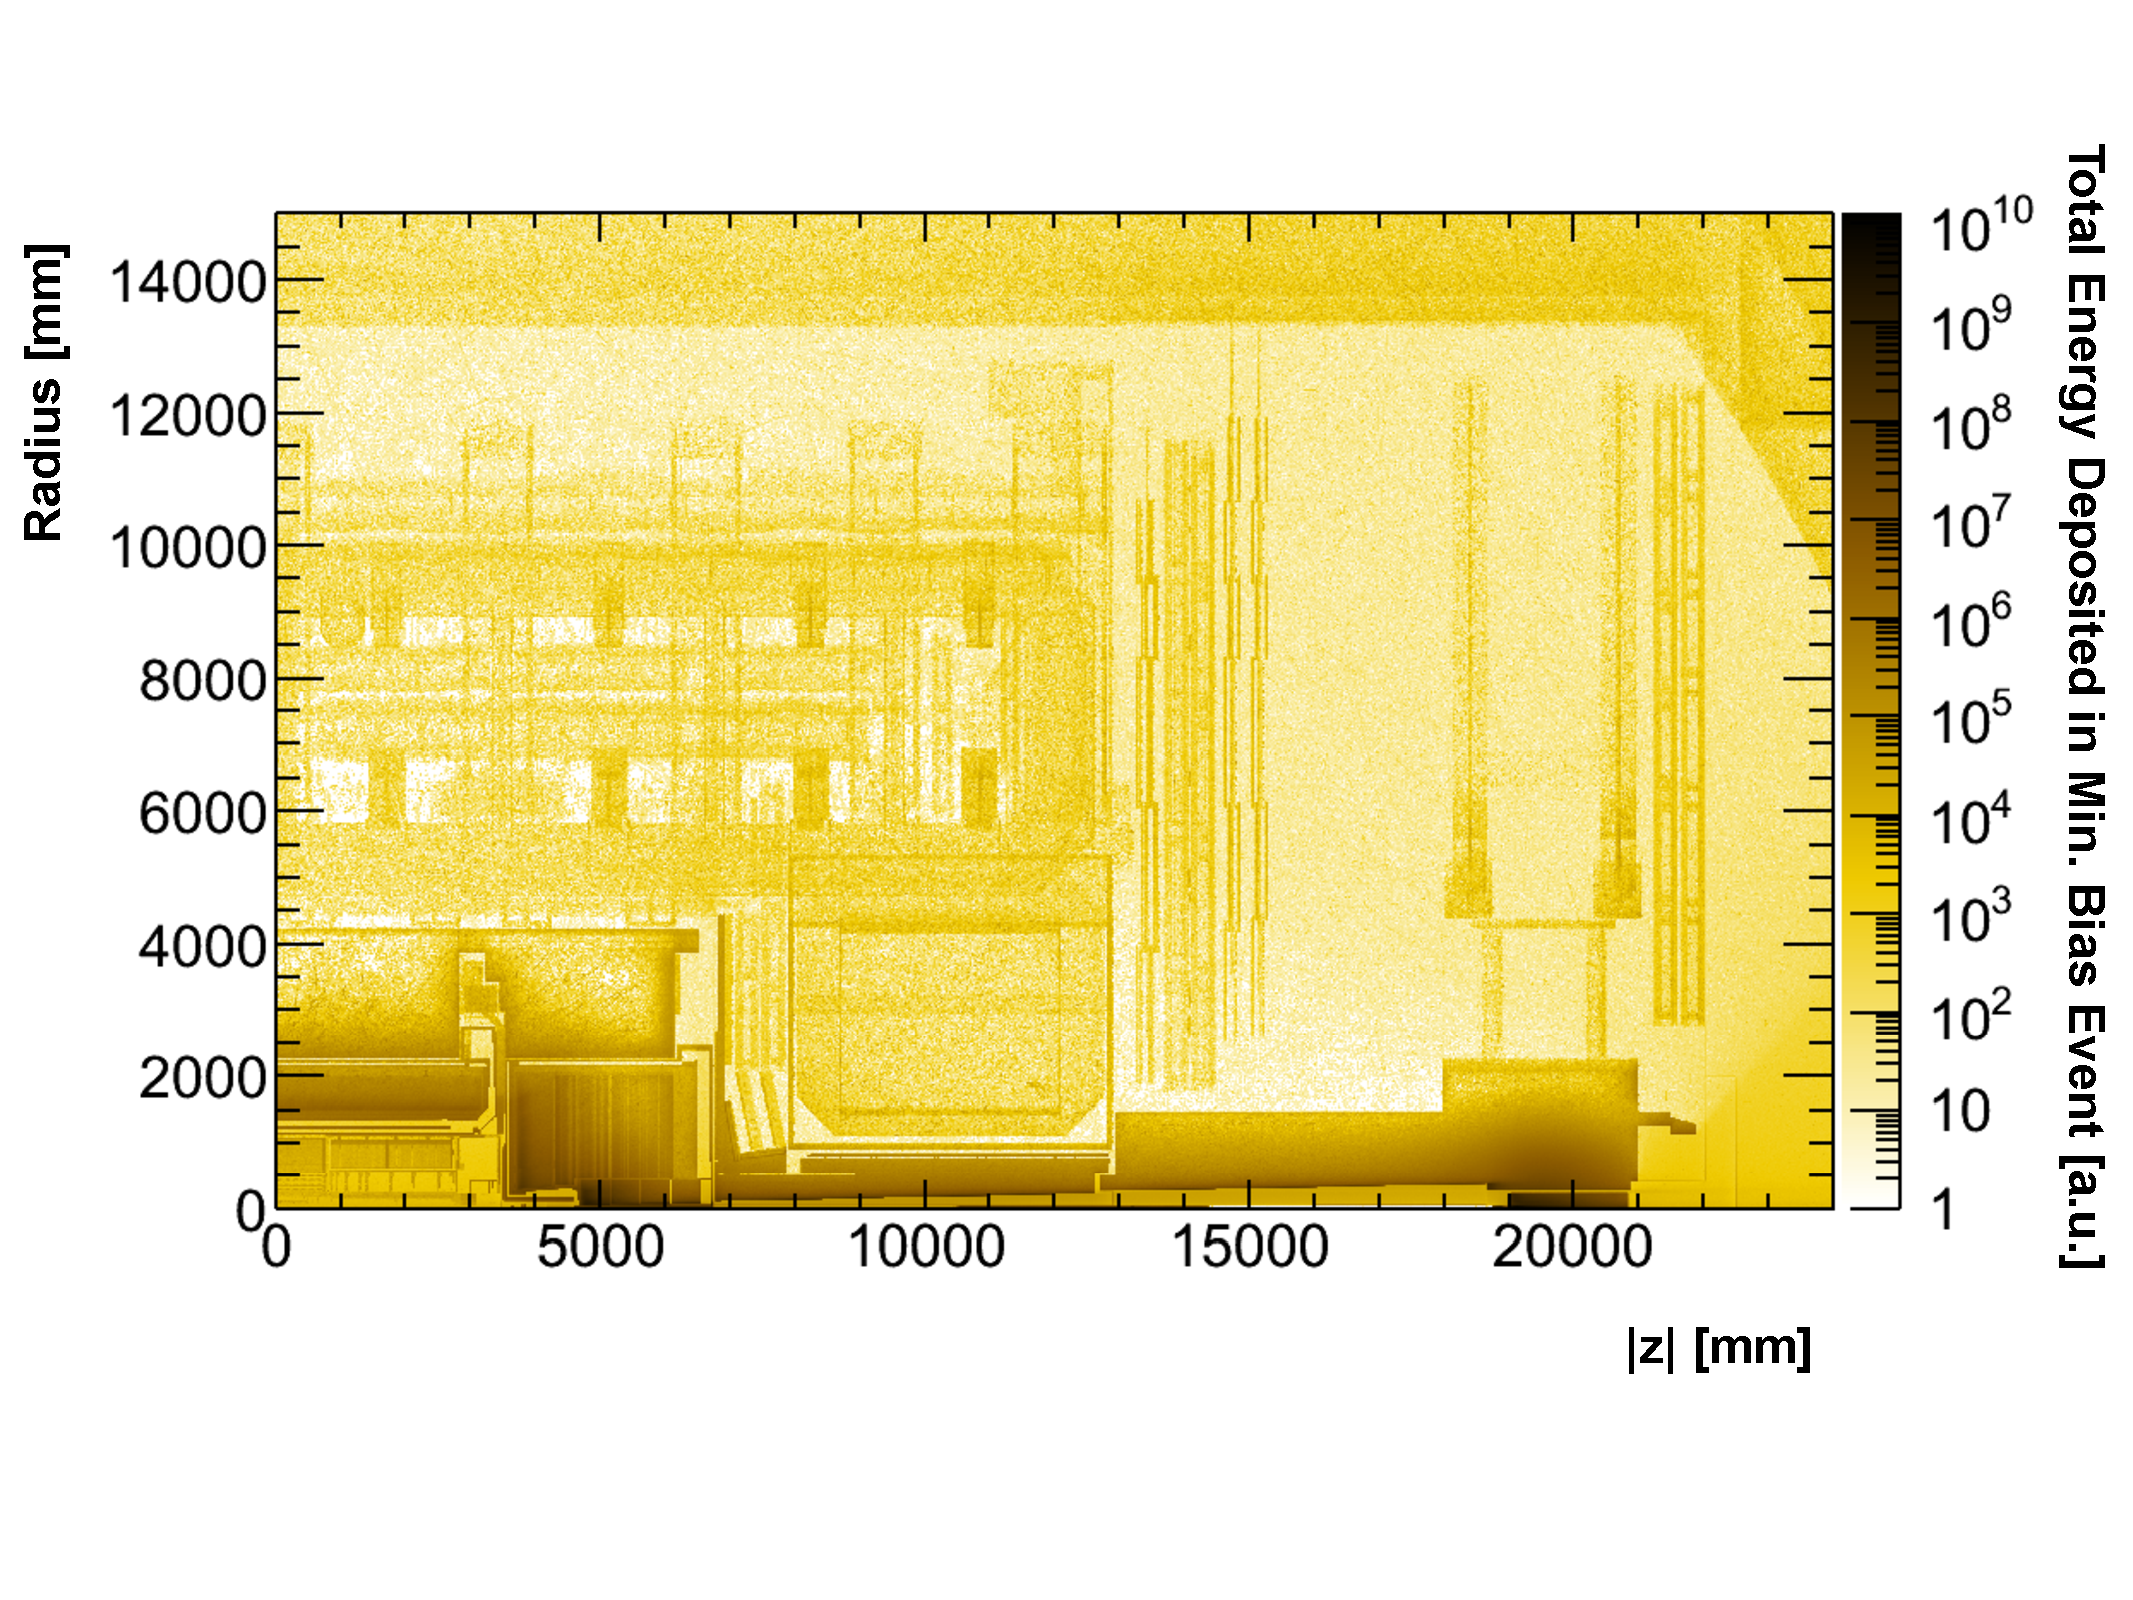
\includegraphics[width=0.8\textwidth]{figures/nsw/atlas_cavern_bkgPDF}
        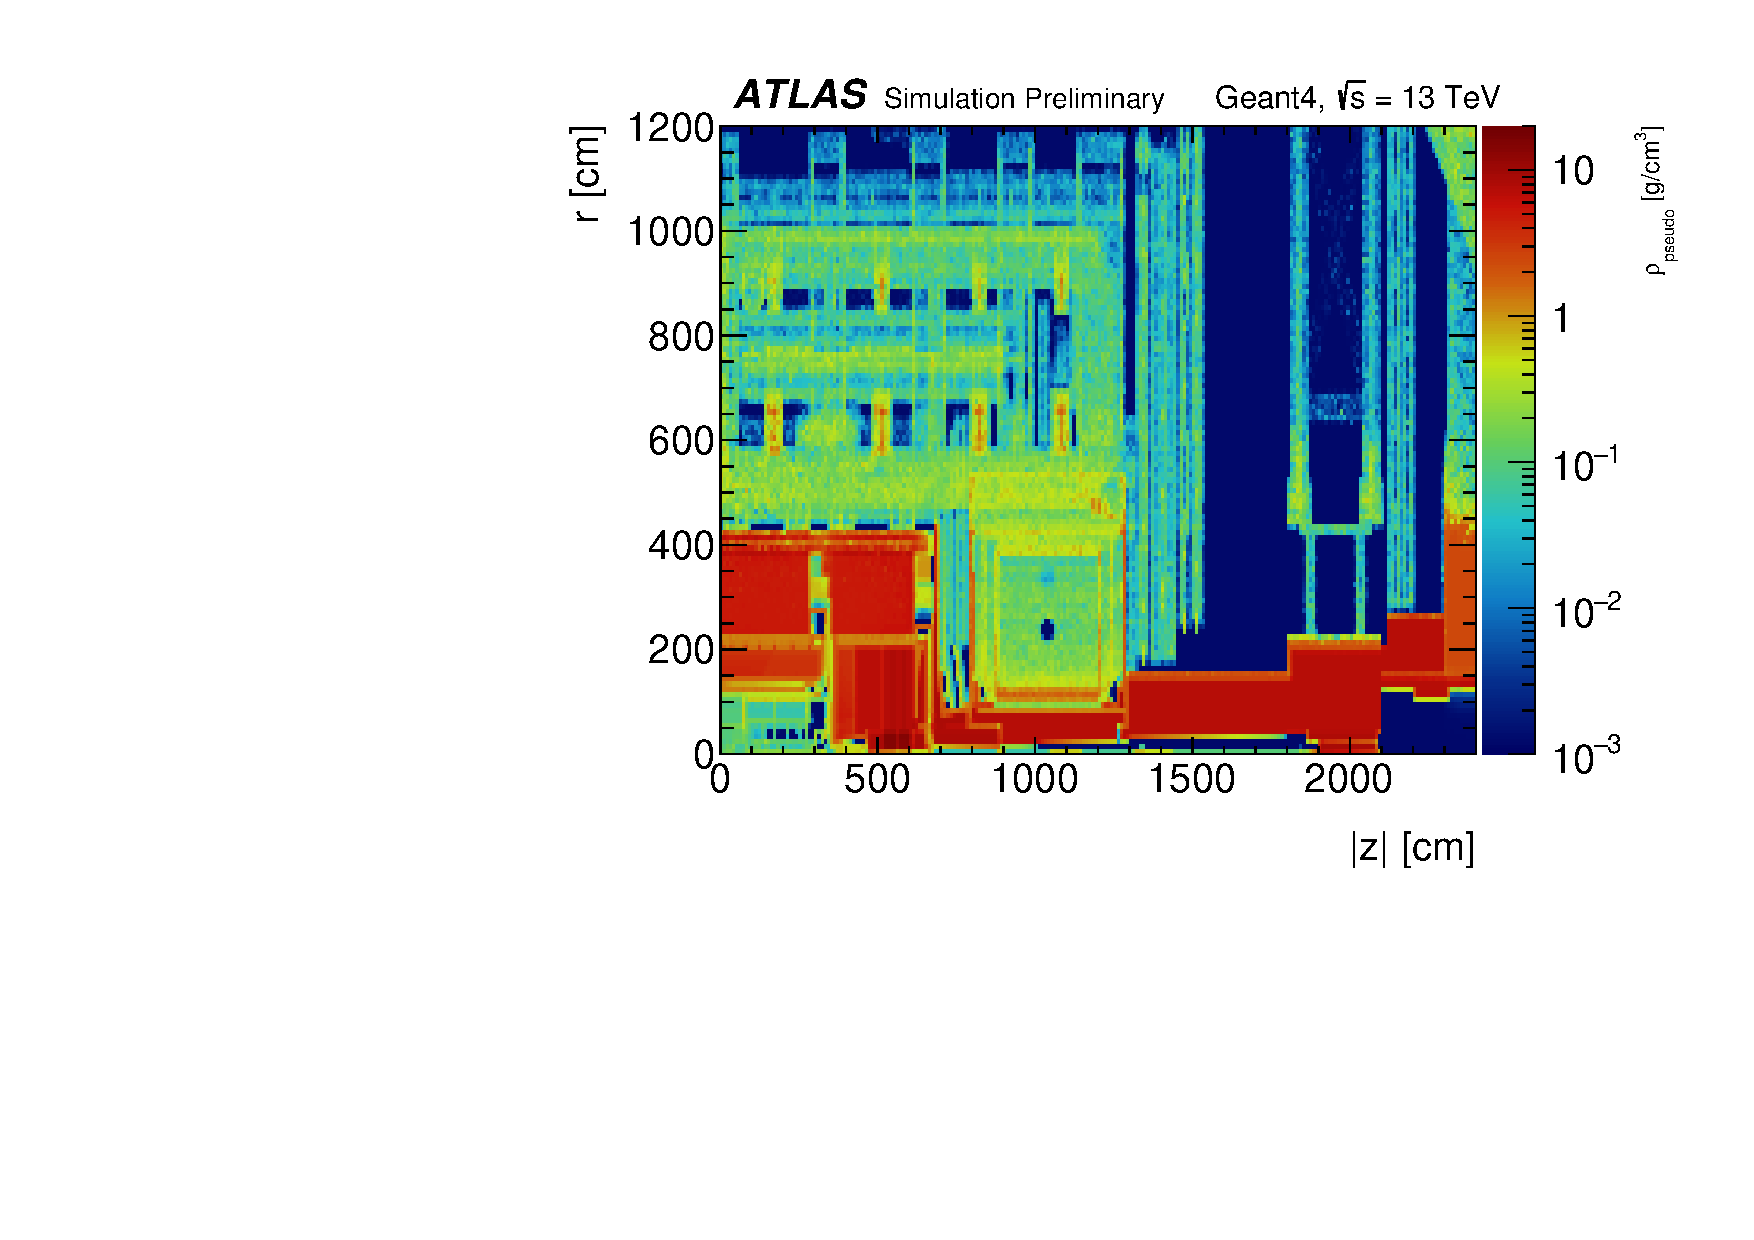
\includegraphics[width=0.8\textwidth]{figures/nsw/atlas_cavern_material_density_sim}
        \caption{
            Simulation of the average material density in materials within a quadrant of the ATLAS cavern.
            %during a minimum bias collision event at $13\,\TeV$.
            %The normalisation of the $z$-axis is arbitrary.
            The forward-calorimeter cryostat, beam-pipe, and shielding ($z\approx 6.8$\,m)
            in front of the Small Wheel experience high energy deposition.
            The largest rates observed by the muon system are those experienced
            by the CSC detectors in the current Small Wheel, which can be seen in the above
            to lie directly behind and above regions of high material interaction.
            Figure taken from Ref.~\cite{ATL-PHYS-PUB-2016-017}.
        }
        \label{fig:cavern_bkg}
    \end{center}
\end{figure}

The NSW will take part in the Level-1 muon trigger by providing
tracking information to aid the TGC-based Level-1 muon trigger logic currently in use for providing
Level-1 muon trigger candidates in the forward region.
The inclusion of such trigger information from the NSW will help to discriminate against
`fake' triggers due to background particles, as illustrated in Figure~\ref{fig:l1mu_rates},
and will also improve the overall muon \pT~measurement in the forward muon trigger which
will enable the Level-1 muon triggers to maintain low \pT-thresholds.
If there were no NSW upgrade, in order to cope with the high rate of Level-1 muon triggers,
the \pT~thresholds of the single-muon triggers would have to be increased from a minimum of $\approx20\,\GeV$
to thresholds well above 40\,\GeV in order to drop the total rate of muon triggers (inclusive of those
in the barrel and end-cap) below the 20\,kHz budget.
Alternatively, the forward muon trigger system could be removed altogether.
In this latter case, all muon triggers would be seeded by Level-1 muon candidates in the barrel only.
Both of these scenarios lead to drastic reduction in physics performance.
Major Higgs-physics goals of ATLAS, for example, would take large hits if either of these
two non-NSW scenarios were enacted.
Increasing the Level-1 muon trigger \pT-thresholds results in a loss in efficiency of more than
30\% for the $Wh,h\rightarrow bb$ process --- a key channel necessary for the observation and study
of the Higgs couplings to $b$-quarks.
A drop in efficiency on the order of 50\% is expected for the same process if the trigger thresholds
are kept low but the forward muon trigger system is removed.
This is illustrated in Figure~\ref{fig:nsw_wh_loss}, both for the $Wh,h\rightarrow bb$ scenario
discussed but also for the $h\rightarrow WW^*$ production channel, an important source of Higgs bosons
in ATLAS.


\begin{figure}[!htb]
    \begin{center}
        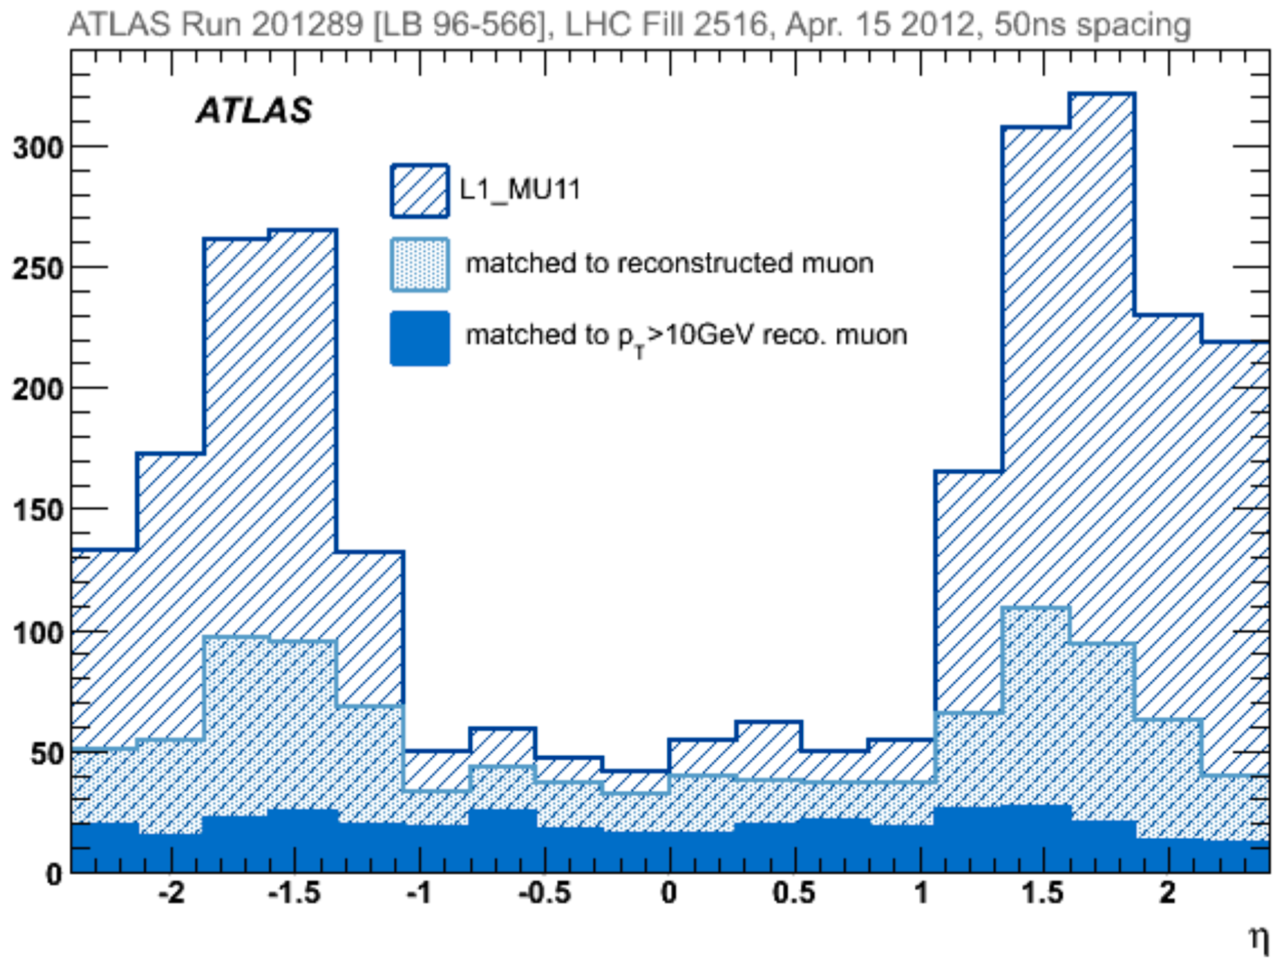
\includegraphics[width=0.47\textwidth]{figures/nsw/nsw_l1mu_rates}
        \raisebox{0.4cm}{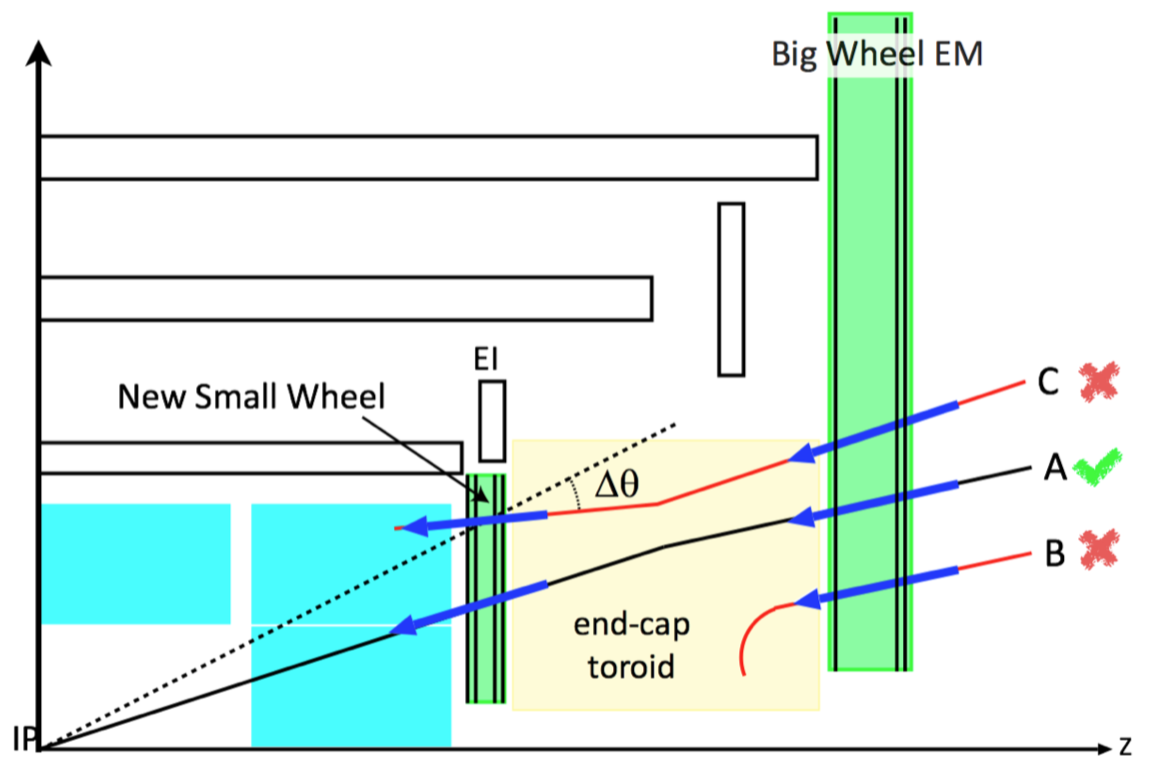
\includegraphics[width=0.5\textwidth]{figures/nsw/nsw_track_principle}}
        \caption{
            Figures taken from Ref.~\cite{NSWTDR}.
            \textbf{\textit{Left}}: Level-1 muon trigger rates as a function of $\eta$. L1\_MU11 refers to the
                rate of the Level-1 accept rate. After requiring that the muon trigger candidates
                responsible for the Level-1 muon trigger firing are matched to a real muon, the
                rate drops significantly, illustrating the rate of `fake' muon triggers in the
                forward muon system.
            \textbf{\textit{Right}}: Illustration of the principle of operation of the NSW trigger system.
                The aim of the NSW trigger is to provide accurate pointing information (via the illustrated $\Delta \theta$ computation) within
                the inner-most muon system to aid the trigger logic of the Big Wheel and thereby reduce the acceptance of `fake' triggers that
                do not have coincident pointing track segments in both wheels.
                With the NSW trigger logic, only the muon trigger candidate labelled `A' will result
                in a Level-1 muon trigger being fired.
                The track candidate `C' (`B') fails to fire a trigger due to non-IP-pointing (missing) track-segments in the NSW,
                characteristic of cavern background particles.
        }
        \label{fig:l1mu_rates}
    \end{center}
\end{figure}

\begin{figure}[!htb]
    \begin{center}
        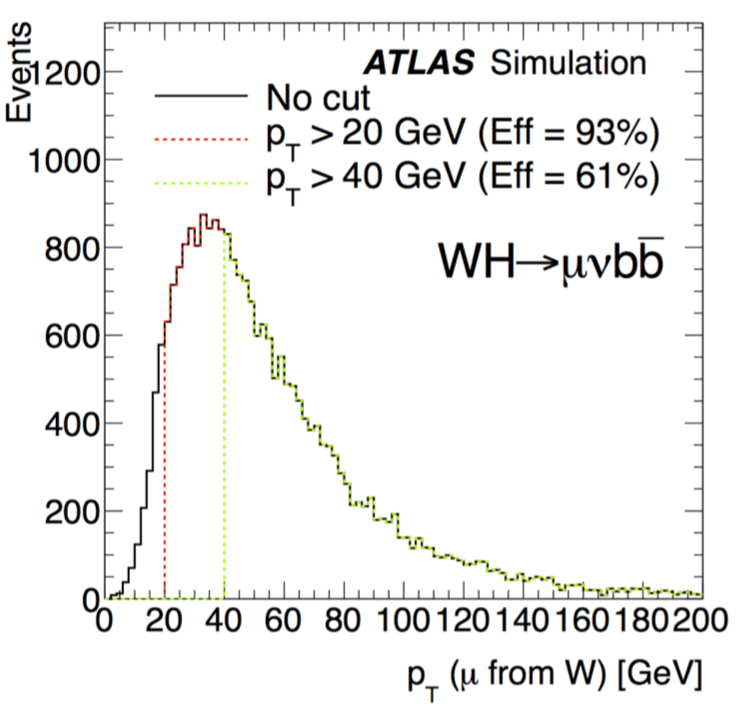
\includegraphics[width=0.4\textwidth]{figures/nsw/nsw_ptmu_wh}
        \raisebox{1.85cm}{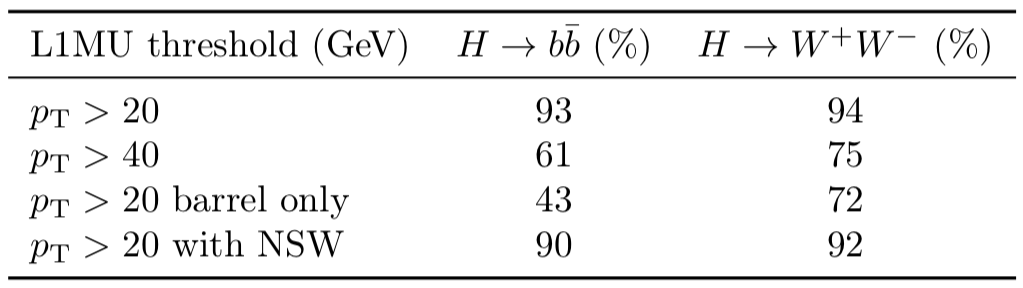
\includegraphics[width=0.55\textwidth]{figures/nsw/nsw_eff_wh_hbb}}
        \caption{
            Figures taken from studies contained in Ref.~\cite{NSWTDR}.
            \textit{\textbf{Left}}: Truth-level \pT~distribution of the trigger-muon in the $Wh$ analysis, showing
                the trigger thresholds and corresponding truth-level selection efficiency of those thresholds.
            \textit{\textbf{Right}}: Selection efficiencies for several trigger-threshold scenarios with and without the NSW
                for the $Wh,h\rightarrow b \bar{b}$ and $h \rightarrow WW^*$ processes.
        }
        \label{fig:nsw_wh_loss}
    \end{center}
\end{figure}

In addition to the trigger performance of the current forward muon system being insufficient
for the foreseen data-taking challenges, the tracking performance of both the MDT and CSC detectors of the current Small Wheel
will also degrade with the increased luminosities.
For example, the MDT detectors are characterised by long signal drift-times that are hundreds of nanoseconds long.
With both these long characteristic drift times and the increased particle rates predicted to occur with the LHC upgrades,
the occupancies that will be experienced by the MDT chambers in the current Small Wheel
will result in significant degradation of their tracking capabilities.
At the high rates expected in the future runs of the (HL-)LHC, the tracking efficiencies
of the MDT chambers will approach 50\% or worse (lower), as illustrated in Figure~\ref{fig:nsw_mdt_track_reco}.
This leads to significant reductions in the capabilities of the inner-most muon stations
in the forward region to provide a third high-resolution muon measurement necessary for the sagitta measurement used for reconstructing
muon momenta.

\begin{figure}[!htb]
    \begin{center}
        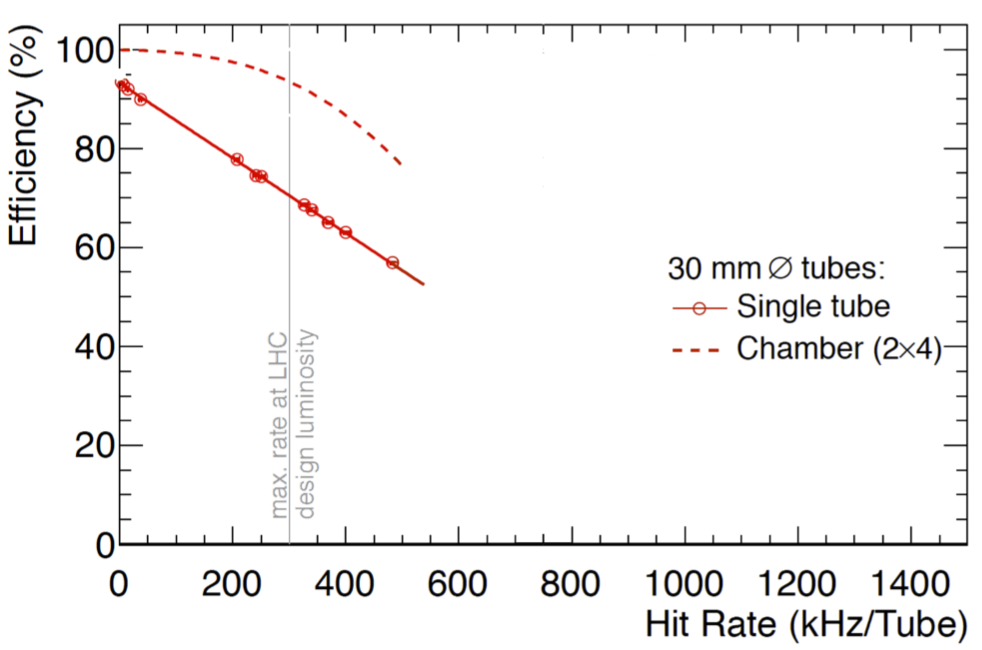
\includegraphics[width=0.7\textwidth]{figures/nsw/nsw_mdt_track_reco_eff}
        \caption{
            Measurements of MDT tube hit (solid line) and track-segment efficiency (dashed-line)
            as a function of tube hit rate.
            The vertical line indicating the maximum LHC rate corresponds to an instantaneous
            luminosity of $1\times10^{34}$cm$^{-2}$s$^{-1}$.
            Figure taken from Ref.~\cite{NSWTDR}.
        }
        \label{fig:nsw_mdt_track_reco}
    \end{center}
\end{figure}


%%%%%%%%%%%%%%%%%%%%%%%%%%%%%%%%%%%%%%%%%%%%%%%%%%%%%%%%%%%%%%%%%%%%%%%
% NSW DETECTOR
%%%%%%%%%%%%%%%%%%%%%%%%%%%%%%%%%%%%%%%%%%%%%%%%%%%%%%%%%%%%%%%%%%%%%%%
\section{The New Small Wheel Detector}
\label{sec:nsw_detector}

%The inability of the current Small Wheel to cope with the foreseen challenges
%of Run 3 and the HL-LHC have been briefly discussed in the
%previous sections.
In this section, a description of the NSW will be presented.
The layout of the NSW will be described in Section~\ref{sec:nsw_geo}
and then a description of the \micromegas (MM)~\cite{Giomataris:1995fq} and Small-strip Thin Gap Chamber (sTGC)
detector technologies that will compose the NSW
will be given in Sections~\ref{sec:nsw_mm} and \ref{sec:nsw_stgc}, respectively.
The MM are throught of as providing primarily high presicion muon tracking
while the sTGC are thought of as primarily providing trigger primitives for the forward Level-1 muon trigger system.
As will be seen, though, both the MM and sTGC technologies will provide both high-quality tracking and trigger primitives.
%The MM detectors are primarily precision tracking detectors and the sTGC
%will serve as trigger detectors, though each provide both tracking and trigger primitives.
The NSW must last for the remainder of the ATLAS detector's lifetime, throughout
both Run 3 and the entirety of the HL-LHC era.
In the following sections, the design decisions of the NSW --- related to both its layout 
and detector choices --- will be presented in light of their ability to address
the particular challenges described in the previous section.

%%%%%%%%%%%%%%%%%%%%%%%%%%%%%%%%%%%%%%%%%%%%%%%%%%%%%%%%%%%%%%%
% NSW GEO
%%%%%%%%%%%%%%%%%%%%%%%%%%%%%%%%%%%%%%%%%%%%%%%%%%%%%%%%%%%%%%%
\subsection{Geometry and Layout}
\label{sec:nsw_geo}

The NSW consists of 16 detector planes, separated into two `multilayers'.
Each multilayer will be composed of four detector planes of each of the two
detector technologies that make up the NSW: the Small-strip Thin Gap Chamber (sTGC)
and MicroMegas\footnote{The name `MicroMegas` is a loose acryonym for `MICROMEsh GAseous Structure'.} (MM)
detectors.
The sTGC are based on multiwire chamber technology and the MM are a type of
micropattern gaseous detector (MPGD)~\cite{MPGD}.
The detectors are arranged into sectors in azimuth, following a similar layout
as the current Small Wheel with alternating large and small sectors, as illustrated in Figure~\ref{fig:nsw_geo}.
The organisation of the detector technologies in each sector is illustrated in Figure~\ref{fig:nsw_sector_layout},
showing the sTGC--MM--MM--sTGC layout of the detector quadruplets, with a $50$\,mm spacer
frame separating the two halves.
Each sector of the NSW will have a length nearing 5\,m, giving the NSW a diameter of
nearly 10\,m.

The current Small Wheel muon system covers the range $1.0 < \lvert \eta \rvert < 2.7$, shown
in Figure~\ref{fig:muon_plan_view_eta}.
The NSW will not cover the entirey of this range, however, and will only cover the
range $1.3 < \lvert \eta \rvert < 2.7$ while the already-existing MDT chambers in the Small Wheel at $1.0 < \lvert \eta  \rvert < 1.3$
will remain in operation after the NSW installation.
The NSW will additionally extend the Level-1 muon trigger system acceptance to include
the region $2.4 < \lvert \eta \rvert < 2.7$, which is currently not the case.

The large number of detection planes provided by the NSW adds a large degree of redundancy
within each of the quadruplets of a given technology: if part of a layer, or even a complete layer,
is non-functioning the remaining layers within the quadruplet will compensate and a loss in performance
will be minimal.
There is additional redundancy provided by the fact that both MM and sTGC detector technologies
will be used for both tracking and trigger functionalities: if an entire or part of a quadruplet
becomes non-functioning, the tracking and/or trigger responsibilities of the lost detector
will be partially covered by the presence of the still-functioning quadruplet(s)/layer(s) of the other
detector technology covering the same or overlapping
$\eta$ range.
%There is additional redundancy provided by the fact that \textit{both} the MM and sTGC detectors
%will provide both tracking and trigger primitives: if an entire or part of a quadruplet becomes
%non-functioning, then the functionalities of the lost detector will be partially covered
%by that of the still-functioning quadruplet(s) in the same $\lvert \eta \rvert$ range.
%That is, although the MM and sTGC are described as being specialised for tracking and trigger functionalities,
%respectively, each technology provides quality inputs for both functions.
The degree of redundancy built into the NSW detector is such that the performance goals
of ATLAS with respect to the forward muon system can be met for the remainder of the experiment's
lifetime of 15 years or more.
With generally few opportunities for meaningful repair and maintenance access, this redundancy is
a necessity for these timescales.

\begin{figure}[!htb]
    \begin{center}
        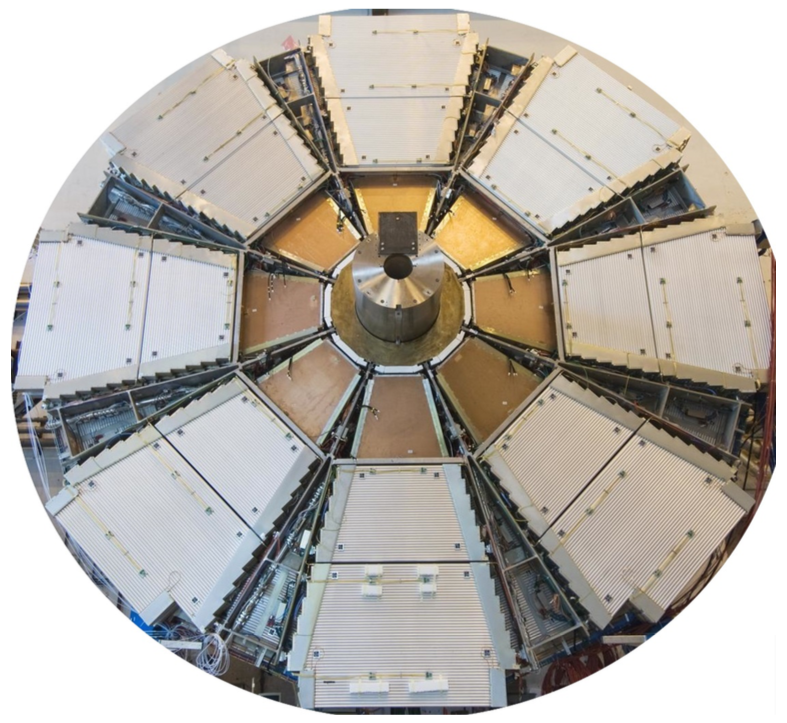
\includegraphics[width=0.48\textwidth]{figures/nsw/nsw_current_sw}
        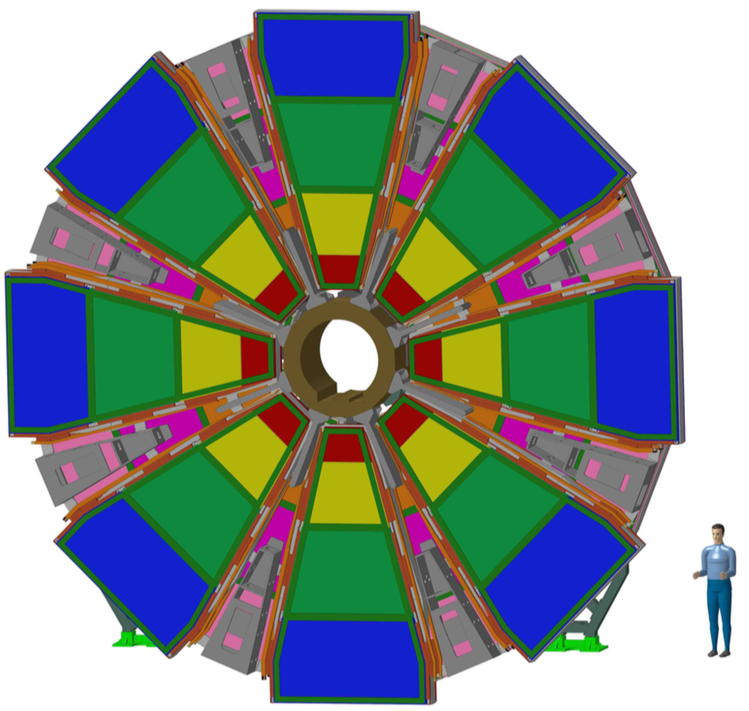
\includegraphics[width=0.48\textwidth]{figures/nsw/nsw_cartoon}
        \caption{
            \textbf{\textit{Left}}: Current Small Wheel detector (prior to installation in ATLAS), with CSC detectors (copper color) at low radii
                and MDT chambers (silver color) at higher radii.
            \textbf{\textit{Right}}: Geometry of the NSW, with a view of the large-sector side. The gaps in azimuth
                between the large sectors are instrumented with detectors on the side facing into the page.
        }
        \label{fig:nsw_geo}
    \end{center}
\end{figure}

\begin{figure}[!htb]
    \begin{center}
        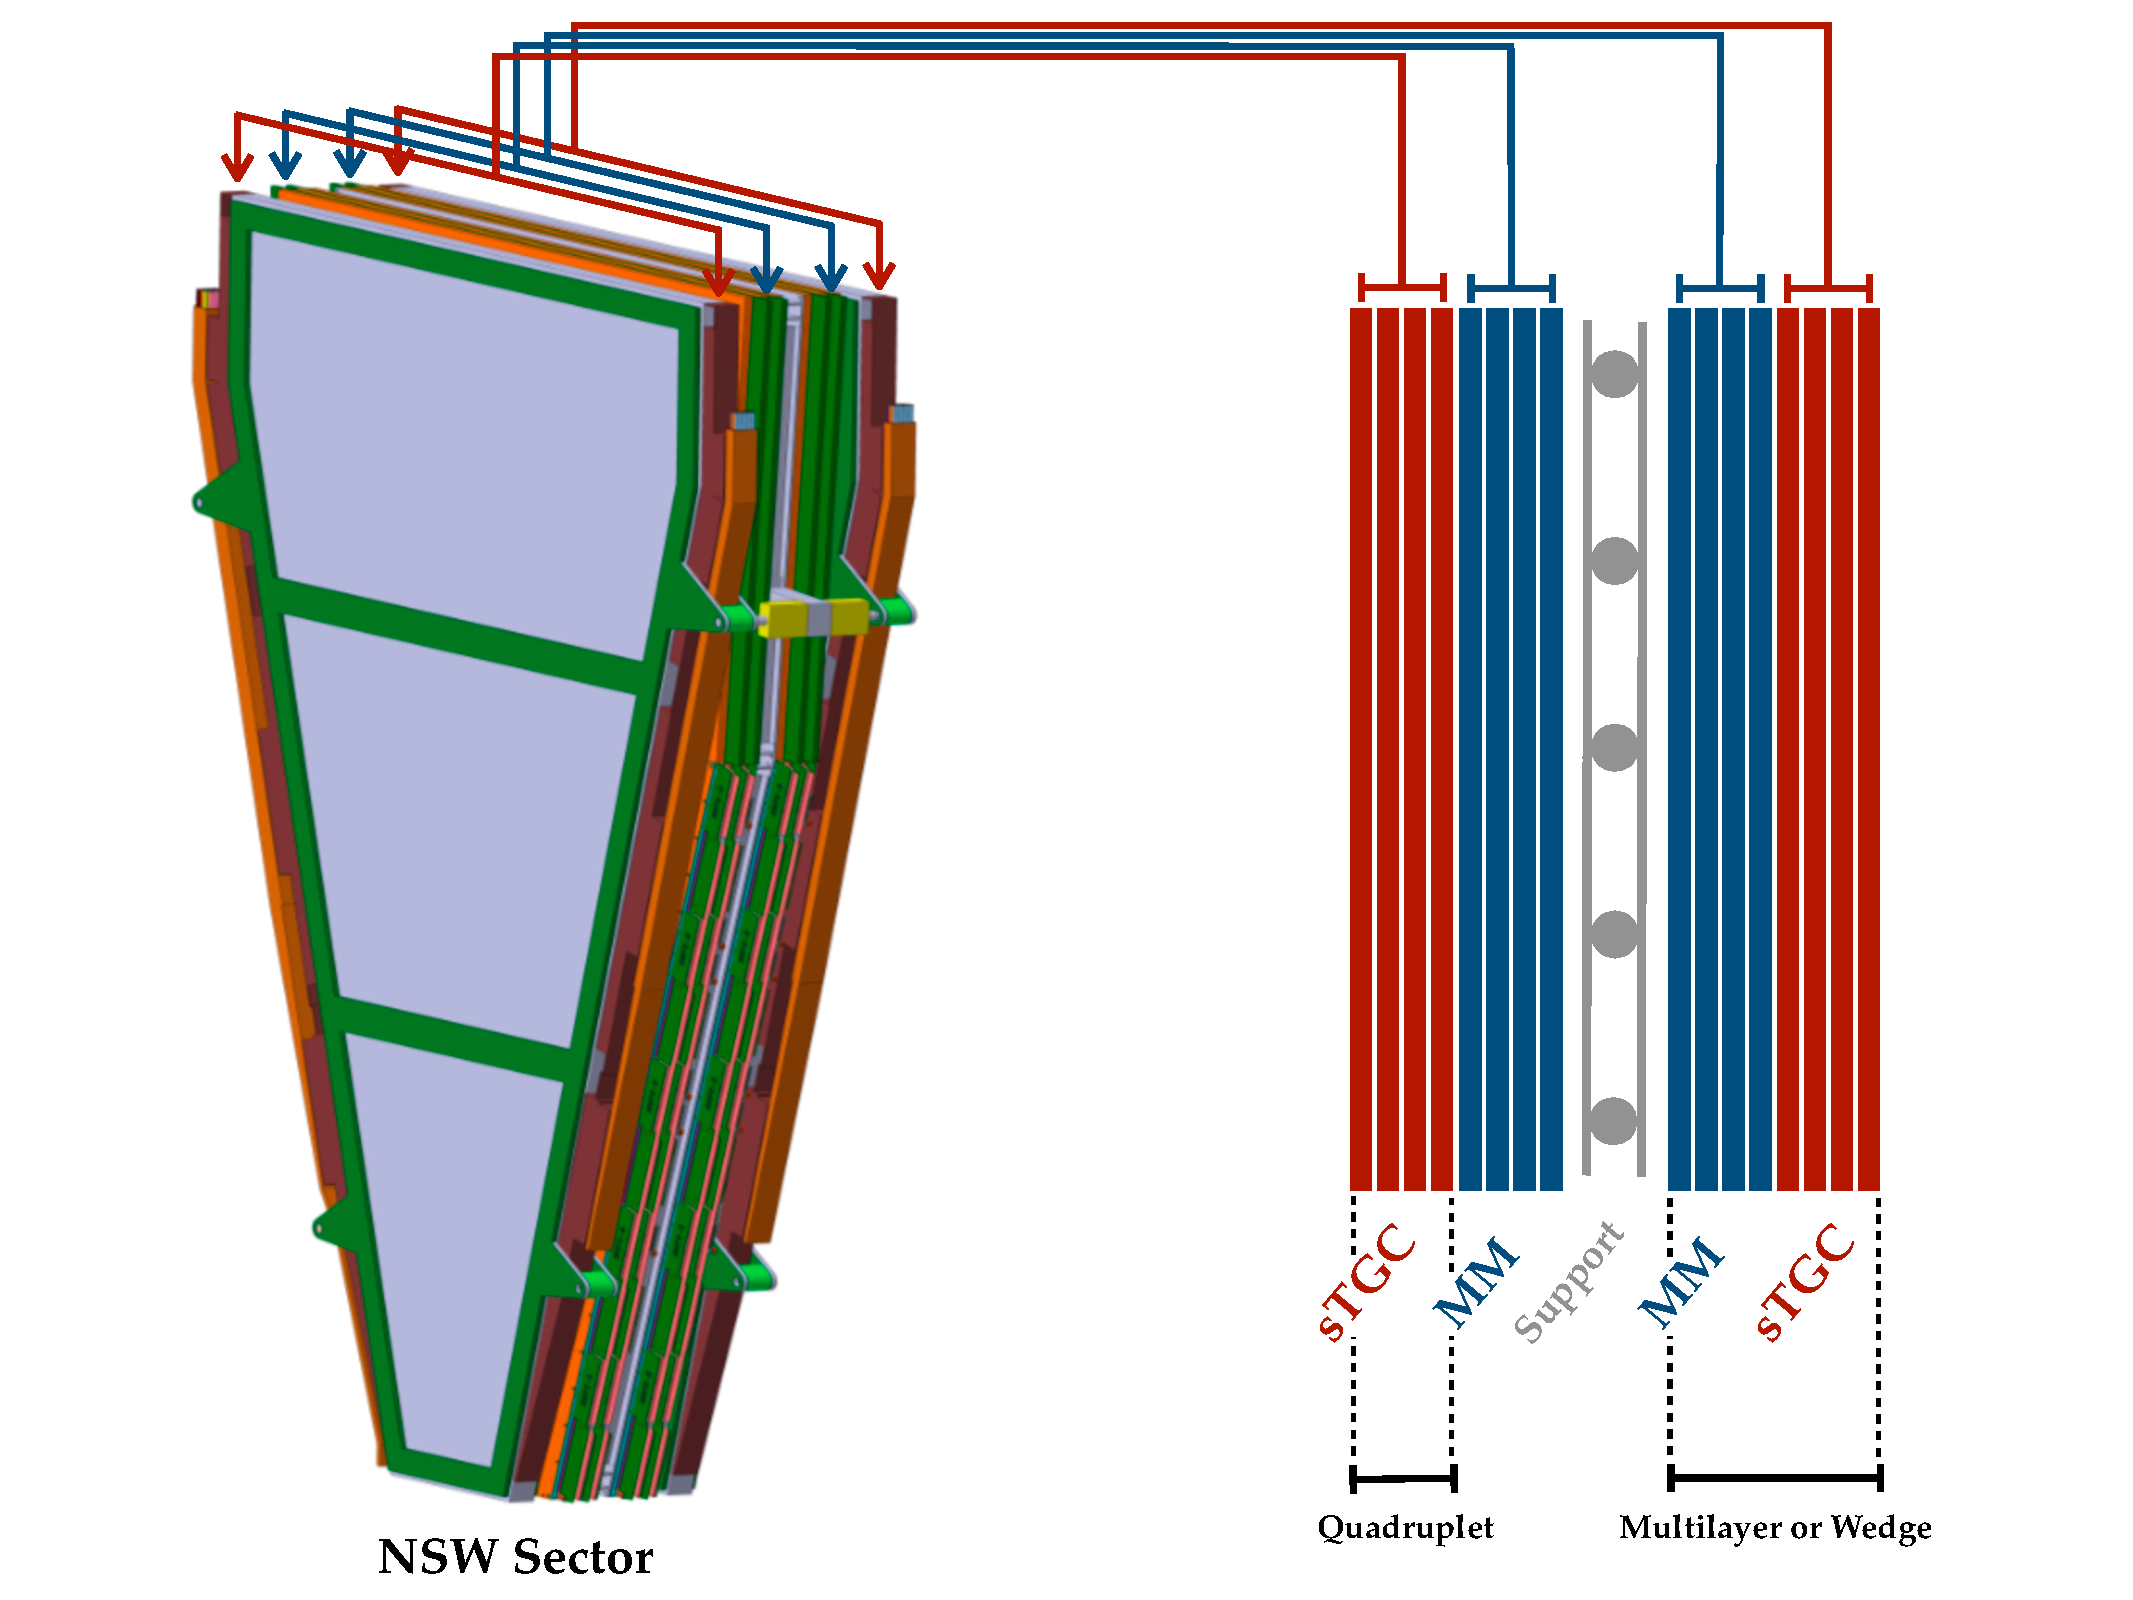
\includegraphics[width=0.8\textwidth]{figures/nsw/nsw_sector_layoutPDF}
        \caption{
            On the left is a mechanical drawing of an NSW sector, with the specific detector
            components illustrated on the right, composed of 16 detector planes: 8 MM layers
            sandwiched between 4 sTGC layers on either side.
            The base component of an NSW detector technology is a single detector plane,
            or layer, four of which are comprised in a single unit referred to as
            a `quadruplet'.
            A single side of the NSW, composed of an MM and sTGC quadruplet, is
            referred to as a `wedge' and a sector is referred to as a `double wedge'.
        }
        \label{fig:nsw_sector_layout}
    \end{center}
\end{figure}

%%%%%%%%%%%%%%%%%%%%%%%%%%%%%%%%%%%%%%%%%%%%%%%%%%%%%%%%%%%%%%%
% MICROMEGAS
%%%%%%%%%%%%%%%%%%%%%%%%%%%%%%%%%%%%%%%%%%%%%%%%%%%%%%%%%%%%%%%
\subsection{The Micromegas Detectors}
\label{sec:nsw_mm}

As mentioned above, the MM detectors are primarily designed with the high-precision tracking
requirements of the HL-LHC in mind, requring a per-layer spatial hit resolution better than $100\,\micron$.
The MM detectors are characterised by readout strips with very fine segmentation and good
time resolution.
Due to this fine time resolution, they will be able to complement the trigger scheme based
on the sTGC detector technology.

%The MM detectors are designed with the high-precision tracking requirements of the HL-LHC
%in mind, requiring a spatial precision better than $100\,\micron$.
%They are characterised by readout strips with very fine segmentation and good
%time resolution and can be exploited to complement the trigger scheme based on the sTGC, as
%described above.

MM detectors are characterised by two asymmetric regions.
The standard MM detector consists of a planar \textit{drift} electrode, a gas gap of
a few millimeters in thickness acting as a conversion and drift region, and a thin
metallic mesh at $\mathcal{O}(100)\,\micron$ above the readout electrodes.
The region between the mesh and readout electrodes is the amplification region wherein
gain factors on the order of $10^4$ are achievable.

The electric potentials within the drift and avalanche regions are maintained
at a few hundred V/cm and $\approx50$\,kV/cm, respectively.
Charged particles traversing the drift space ionise the gas and the electrons, liberated
in the ionisation process, drift towards the mesh at timescales on the order of tens of nanoseconds.
The electron avalanche takes place in the amplification region in about a nanosecond,
resulting in a fast current pulse on the readout electrode.

The MM detectors in the NSW are \textit{resistive-strip} MM detectors, characterised by an insulating
layer over the readout electrodes.
The insulating layer acts to protect the sensitive readout electrodes from sparking events that
reduce the detector performance over time and that are expected to happen frequently given
the very large gas amplification.
%Such sparking events can happen frequently given the very large gas amplifications and high electric potentials
%present in the amplification region.
Resistive strips on top of the insulating layer collect the avalanche electrons and induce
signals on copper readout strips embedded beneath the insulating layer.
The geometry (strip pitch and width) of the copper readout strips need not necessarily be the
same as that of the resistive strips.
Resistrive-strip MM detectors are able to sustain higher amplification and particle rates, a necessary
characteristic for targetting the high-luminosities foreseen at the HL-LHC.
The design and principle of operation of the resistive-strip MM technology is shown in Figure~\ref{fig:nsw_mm_principle},
in which incident MIPs traversing perpendicular and at an angle relative to the detector plane
are illustrated.

Each layer of an MM detector in the NSW is composed of $1024 \times 8$ parallel readout strips, giving
a highly granular spatial readout allowing for high resolution position measurements to be made.
Although all readout strips of a given MM layer are parallel, the MM quadruplets will be capable
of two-dimensional readout and will provide both $r$ and $\phi$ coordinate information
of traversing particles.
The two dimensional readout is achieved through the use of a small-angle stereo readout, in which
MM layers are tilted by fixed relative angles of $\pm 1.5$\,degrees.
This means of a two-dimensional readout is unlike that achieved by the CSC detectors in the current
Small Wheel, in which the readout plane consists of perpendicular wires and strips providing
the two dimensional readout information.
This perpendicular readout is susceptible to high rates of so-called \textit{ghost hits},
illustrated in the left side of Figure~\ref{fig:mm_stereo}, and leads to high levels of track-building ambiguities.
In the high particle rates expected at the HL-LHC, the multiplicies of these ghost hits would
lead to an unacceptable degradation in tracking performance.
The combination of the small-angle stereo readout and high strip-multiplicities on each MM layer will
enable the MM detectors to sustain these high particle rates.
In the right side of Figure~\ref{fig:mm_stereo}, the layout of the MM layers in the NSW as regards
their readout strip orientation (i.e. tilted or not) is illustrated.

Typical definitions of hit locations within strip-based detectors are based on the
centroid method, using the charge-weighted strip position to define the spatial location
of the hit.
This method works optimally for particles incident at angles perpendicular (zero inclination) to the detector readout plane.
The planar NSW detectors, however, will be subjected to particles originating from the IP that follow inclined tracks.
The centroid method provides worsening spatial resolution as the incident angles of these inclined tracks increase due
to the charges from the multiple ionisation events of a single incident particle being spread across multiple readout strips (Figure~\ref{fig:nsw_mm_principle}).
To overcome this, the MM hit reconstruction will use hit timing information
to use the $5$\,mm conversion gap as a time-projection chamber (TPC).
In the NSW, this two-dimensional TPC hit reconstruction is referred to as the micro-TPC (`$\mu$-TPC') reconstruction method.
The use of the timing information of each of the hits recorded by the readout strips
allows for the position above the readout plane to be reconstructed, thereby
allowing for a mini-track to be reconstructed that follows the ionisation history
of a single incident particle.
From this mini-track, a well-defined metric for defining the hit location for inclined tracks on
each MM layer can be defined, as illustrated on the left side of Figure~\ref{fig:mm_tpc_hit_loc}.
In the NSW, the MM hit location will be determined through the combined use of both the
charge-centroid and $\mu$-TPC methods, allowing for sufficient spatial resolution spanning the relevant
incident angles, as illustrated on the right side of Figure~\ref{fig:mm_tpc_hit_loc}.
%This combined 
%From this mini-track a well-defined metric for defining the hit location for inclined tracks on each MM layer can be defined,
%as illustrated in Figure~\ref{fig:mm_tpc_hit_loc}.


\begin{figure}[!htb]
    \begin{center}
        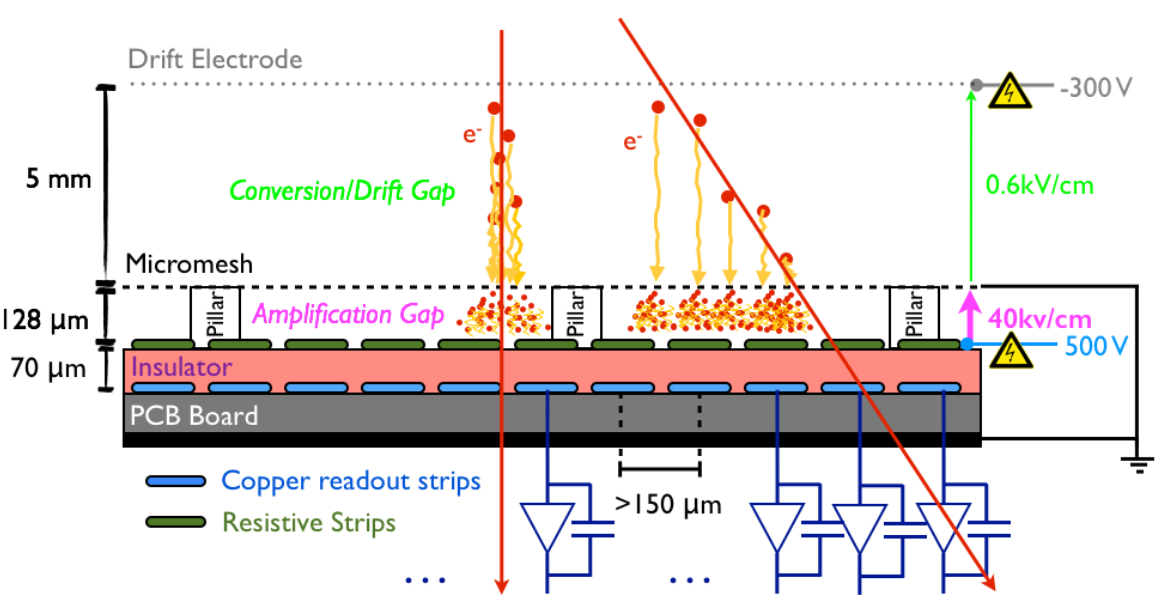
\includegraphics[width=0.75\textwidth]{figures/nsw/nsw_mm_principle}
       % \raisebox{1.12cm}{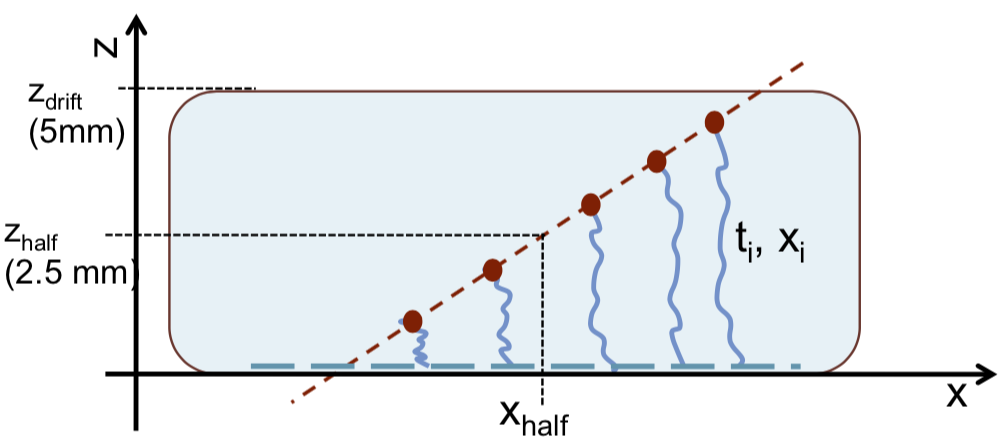
\includegraphics[width=0.37\textwidth]{figures/nsw/mm_tpc_hit_loc}}
        \caption{
        }
        \label{fig:nsw_mm_principle}
    \end{center}
\end{figure}

\begin{figure}[!htb]
    \begin{center}
        %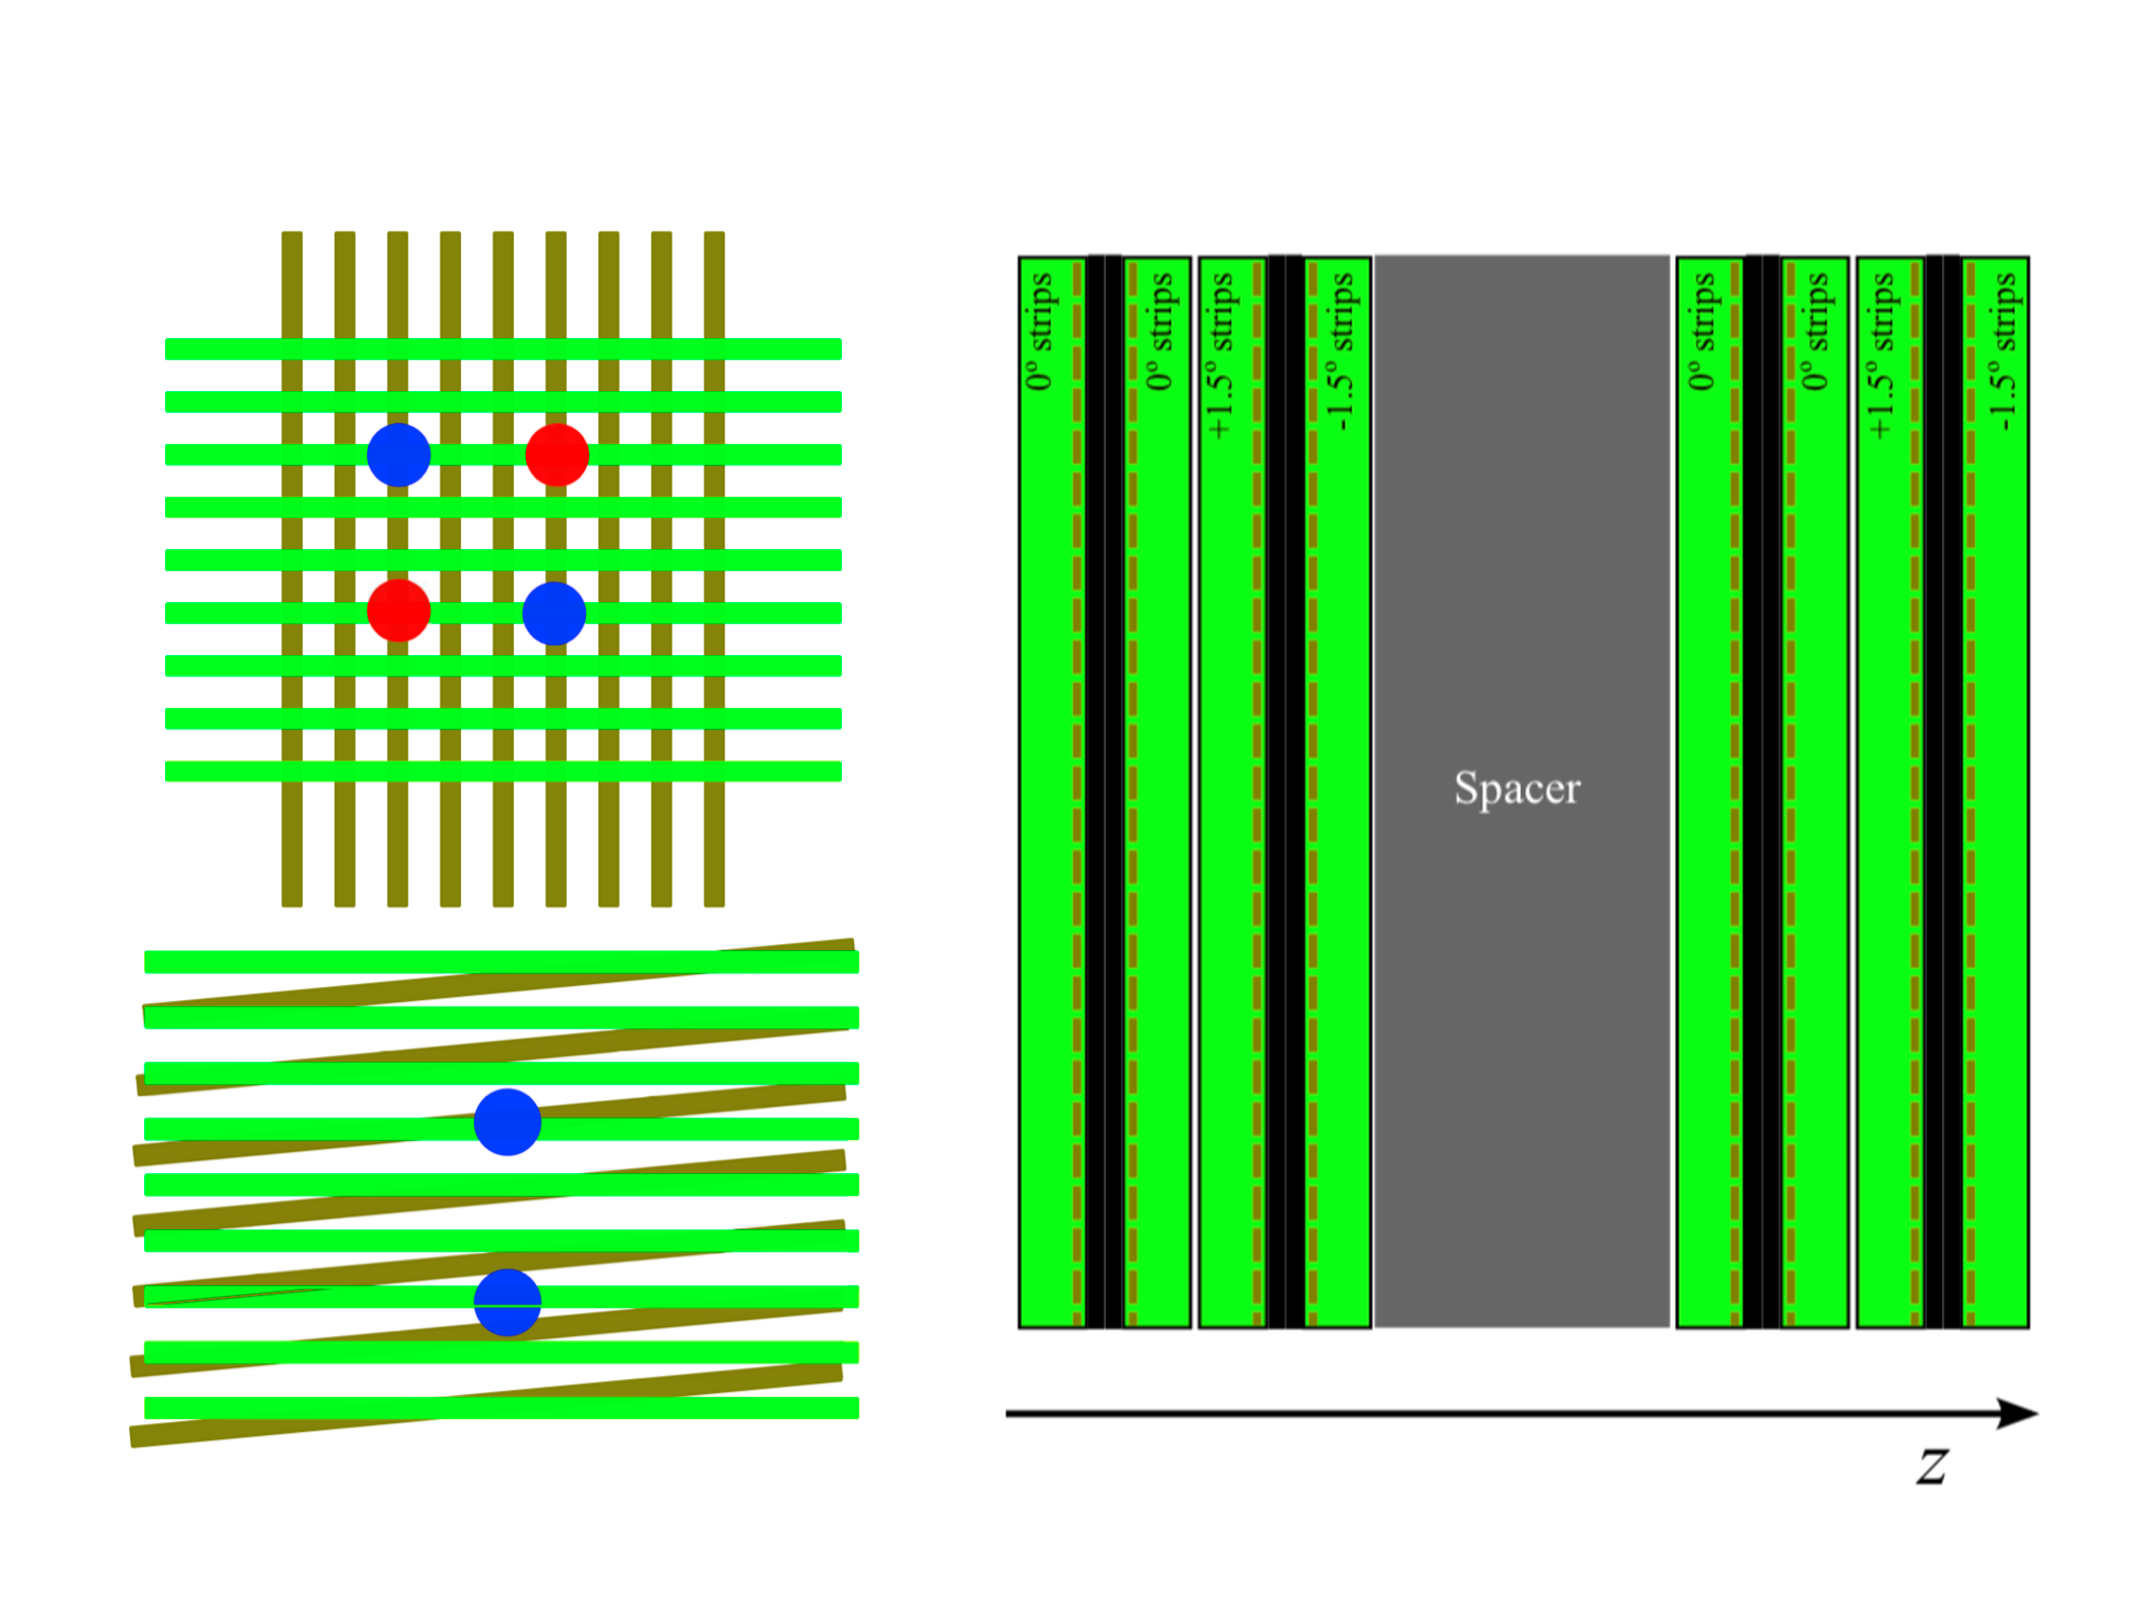
\includegraphics[width=0.8\textwidth]{figures/nsw/mm_ghost_stereoPDF}
        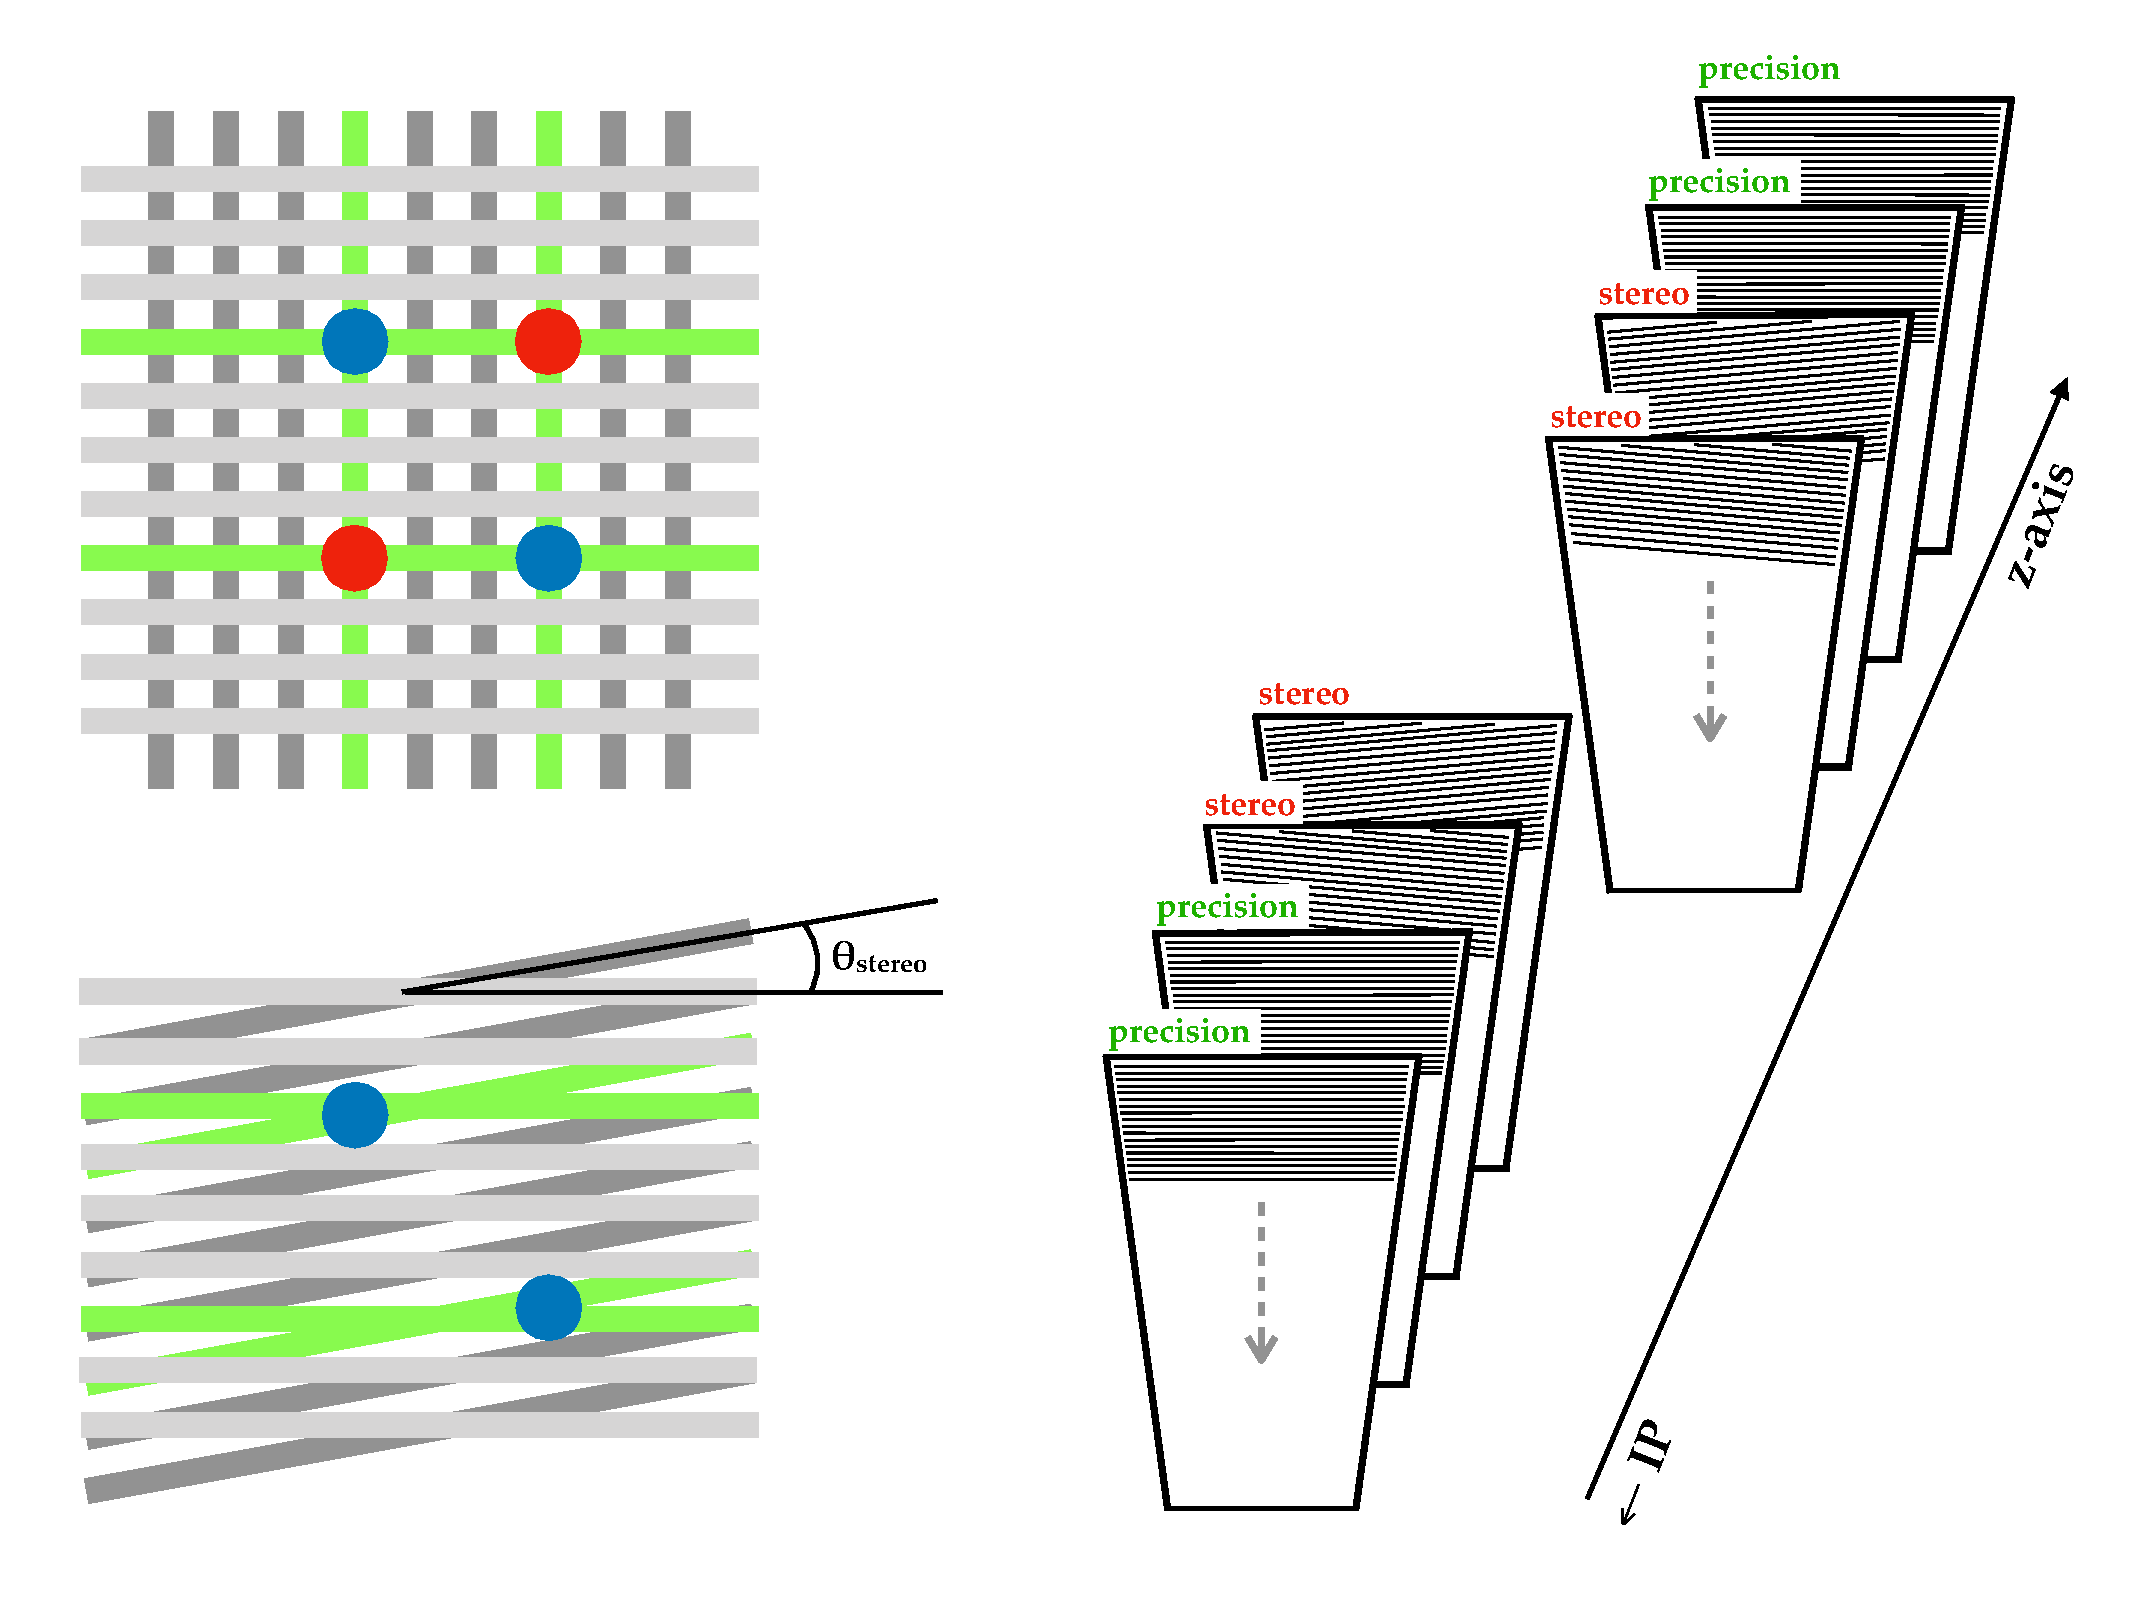
\includegraphics[width=0.8\textwidth]{figures/nsw/mm_stereo_cartoonPDF}
        \caption{
            \textbf{\textit{Left}}: Illustration of the small-angle stereo two-dimensional readout principle.
                The upper panel shows two layers with readout strips perpendicular to each other.
                The lower panel shows two layers with readout strips tilted at a small-angle,
                $\theta_{\text{stereo}}$, relative to one another.
                In both cases, true detector hits are indicated by the blue dots.
                The readout strips registering the hits are indicated in green.
                In the case with perpendicular readout, there are two ghost hits indicated
                by the red dots.
                For perpendicular readout strips, there will generally be $N_{\text{ghost}} = (N^2 - N)$
                ghost hits for $N$ real hits when the readout strips on the two layers have
                equal pitches as in the case of the MM detectors in the NSW.
                On the lower panel, the green readout strips registering the two hits
                do not cross as a result of the small stereo angle and there are no ghost hits.
            \textbf{\textit{Right}}: Illustration of the layout of the `precision' and `stereo'
                readout layers of the two MM quadruplets in a given NSW sector.
                The precision layers, so-called since their readout strips are along $\phi$ and measure directly the
                coordinate in the bending plane of passing muons, are the outer two layers of
                each quadruplet relative to the spacer frame.
                The stereo layers are those with the readout strips tilted at $\pm 1.5^{\degree}$ relative to the precision layers and are the two layers
                in each quadruplet nearest the central spacer frame.
                One stereo layer in each quadruplet has stereo angle $+1.5^{\degree}$ and the other $-1.5^{\degree}$, making
                for $\Delta \theta = 3^{\degree}$ between the two stereo layers.
        }
        \label{fig:mm_stereo}
    \end{center}
\end{figure}

\begin{figure}[!htb]
    \begin{center}
        \raisebox{1.4cm}{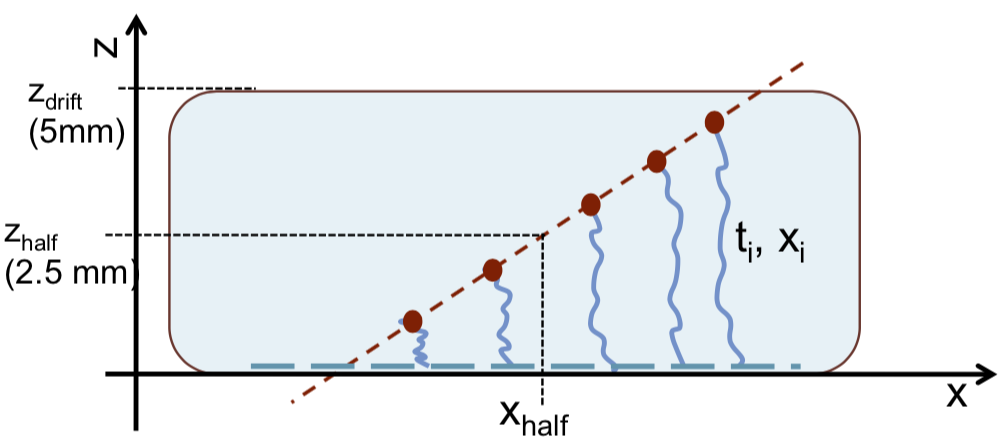
\includegraphics[width=0.48\textwidth]{figures/nsw/mm_tpc_hit_loc}}
        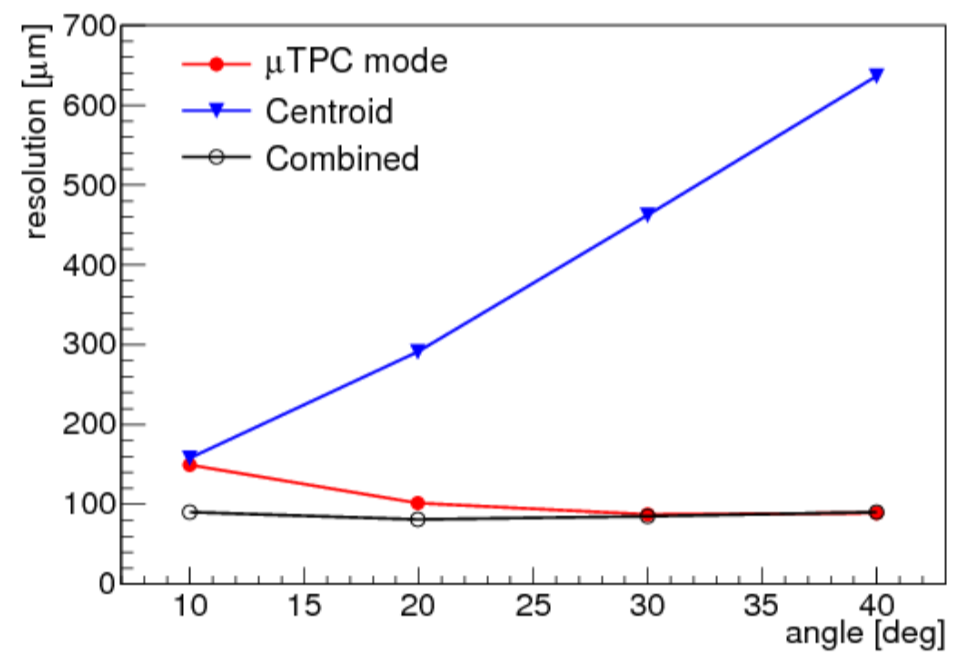
\includegraphics[width=0.48\textwidth]{figures/nsw/tpc_vs_centroid_res}
        \caption{
            \textit{Left}: Illustration of the `$x_{\text{half}}$' method of defining a hit position for
                an inclinded track: the hit position is defined as the position on the readout plane
                corresponding to the half-height location along the reconstructed tracklet in the MM conversion gap.
            \textit{Right}: Expected MM spatial resolution with charge centroid method (blue triangles), $\mu$-TPC
                method (filled red circles), and the combination of the two (black open circles) as a function
                of particle incident angle.
                The combination of the two methods achieves the greater-than $100\,\micron$ single-layer spatial resolution
                required for HL-LHC operation for the expected range of incident angles.
        }
        \label{fig:mm_tpc_hit_loc}
    \end{center}
\end{figure}

%%%%%%%%%%%%%%%%%%%%%%%%%%%%%%%%%%%%%%%%%%%%%%%%%%%%%%%%%%%%%%%
% STGC
%%%%%%%%%%%%%%%%%%%%%%%%%%%%%%%%%%%%%%%%%%%%%%%%%%%%%%%%%%%%%%%
\subsection{The Small-strip Thin Gap Chamber Detectors}
\label{sec:nsw_stgc}

The sTGC are those detectors stated as being primarily used for producing trigger primitives
to be used by the Level-1 muon trigger system.
As triggering detectors, they have fast signal formation and readout times owing to their characteristic high
operating electric fields.
This enables
them to provide accurate bunch crossing identification (i.e. assigning hits to a specific bunch crossing).
The average drift time of ionisation electrons within the sTGC chambers is less than 25\,ns,
with the earliest cluster arrival times well below 10\,ns.
Figure~\ref{fig:stgc_timing} shows the distribution of the measured drift times in an
sTGC, with 95\% of the measured and simulated data being inside a 25\,ns (the LHC bunch crossing
frequency) time window.
The sTCG detectors also provide good online angular resolution --- better than 1\,mrad --- for the track segments
reconstructed across the layers of an sTGC quadruplet, meaning fairly good spatial resolution.
The high quality angular resolution allows for good \pT~determination based on the trigger primitives
provided to the Level-1 trigger.
Offline spatial reconstruction for track segments provided by the sTGC detectors will also be good, matching
the sub-100$\,\micron$ threshold for the HL-LHC precision tracking requirements in the forward region
of the muon system.

\begin{figure}[!htb]
    \begin{center}
        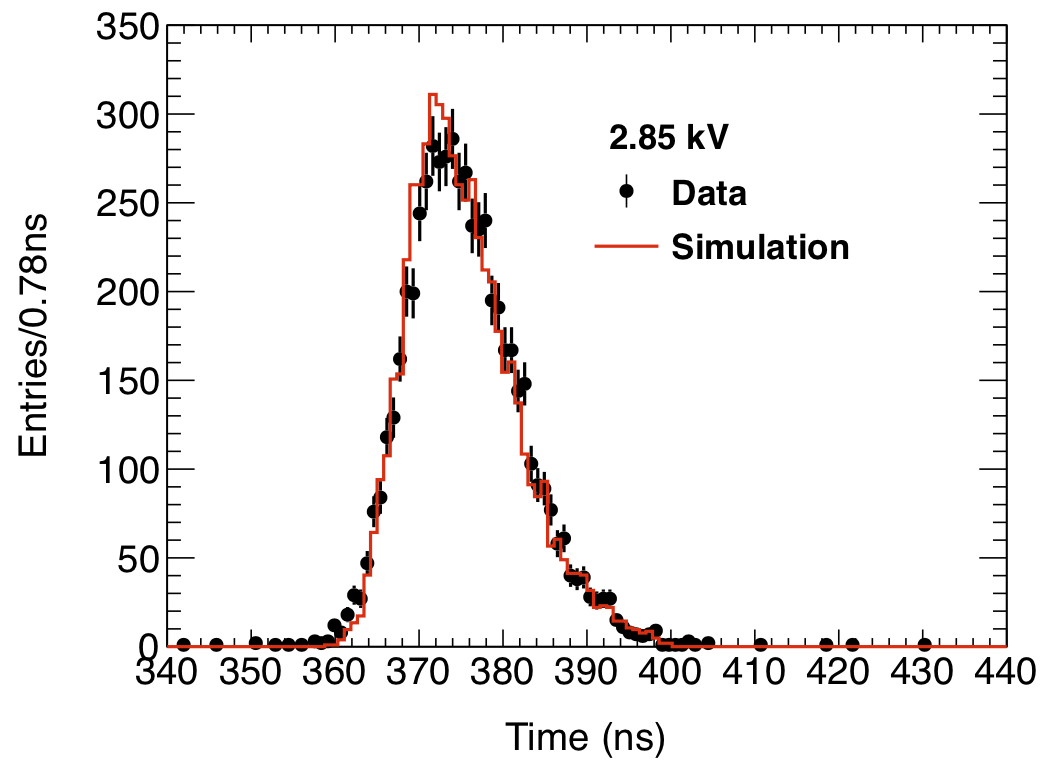
\includegraphics[width=0.5\textwidth]{figures/nsw/stgc_timing}
        \caption{
            Due to the very thin gap and the intense electric field applied,
            $\approx95$\,\% of the measured drift times of passing MIPs are
            confined within a window of 25\,ns, showing that the sTGC
            are capable of relaible bunch crossing assignment.
        }
        \label{fig:stgc_timing}
    \end{center}
\end{figure}

The basic sTGC detector is shown in Figure~\ref{fig:stgc_drawing}.
It consists of a grid of $50\,\micron$ gold-plated tungsten wires with $1.8$\,mm pitch
sandwiched between two cathode planes at a distance of $1.4$\,mm.
On one plane there are the readout pads and on the other the strips.
The strips have a $3.2$\,mm pitch, which is smaller than that of the current TGC
detectors used in the current forward muon system (Figure~\ref{fig:muon_plan_view_eta}),
which is the origin of the name of the sTGC detectors.
The wires and strips are perpendicular, with the wires stretching along $r$ and the
strips along $\phi$.

The pads are used to form coincidences between the layers of the sTGC quadruplets in order
to form projective trigger primitives corresponding to muon tracks pointing roughly back to the IP.
There are $\approx 1300$ pads per sTGC layer.
The collected charge from all components of the sTGC --- the pads, strips, and wires --- associated with a traversing particle are read out and
used for the subsequent offline precision muon-track reconstruction.
Two-dimensional readout is achieved by the $r$ and $\phi$ information provided by the strips
and wires, respectively.
To help cope with the foreseen high particle rates, and to reduce the types of tracking ambiguities
described in Section~\ref{sec:nsw_mm} due to combinatorial hits, only
those wires and strips covering the projective area of pads registering the passage of
the particle are read out.
Additionally, wires are grouped together (i.e. multiple wires correspond to a single readout
channel) as only a rough measurement of the azimuthal coordinate --- not relevant for \pT~determination in the trigger---
is needed.
With the charge information collected from the three sub-components, the sTGC is able to achieve very
good spatial resolutions approaching $approx 80\,\micron$ ($\approx 100\,\micron$) per layer for perpendicular (inclined) tracks.

\begin{figure}[!htb]
    \begin{center}
        \raisebox{0.8cm}{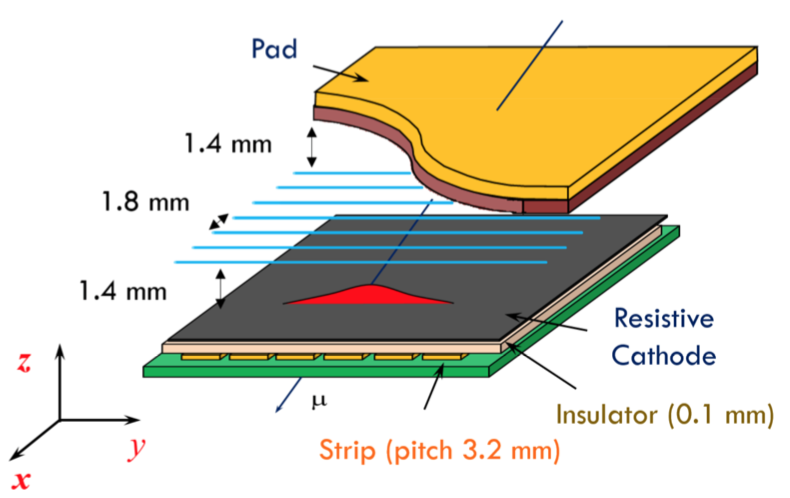
\includegraphics[width=0.52\textwidth]{figures/nsw/stgc_drawing}}
        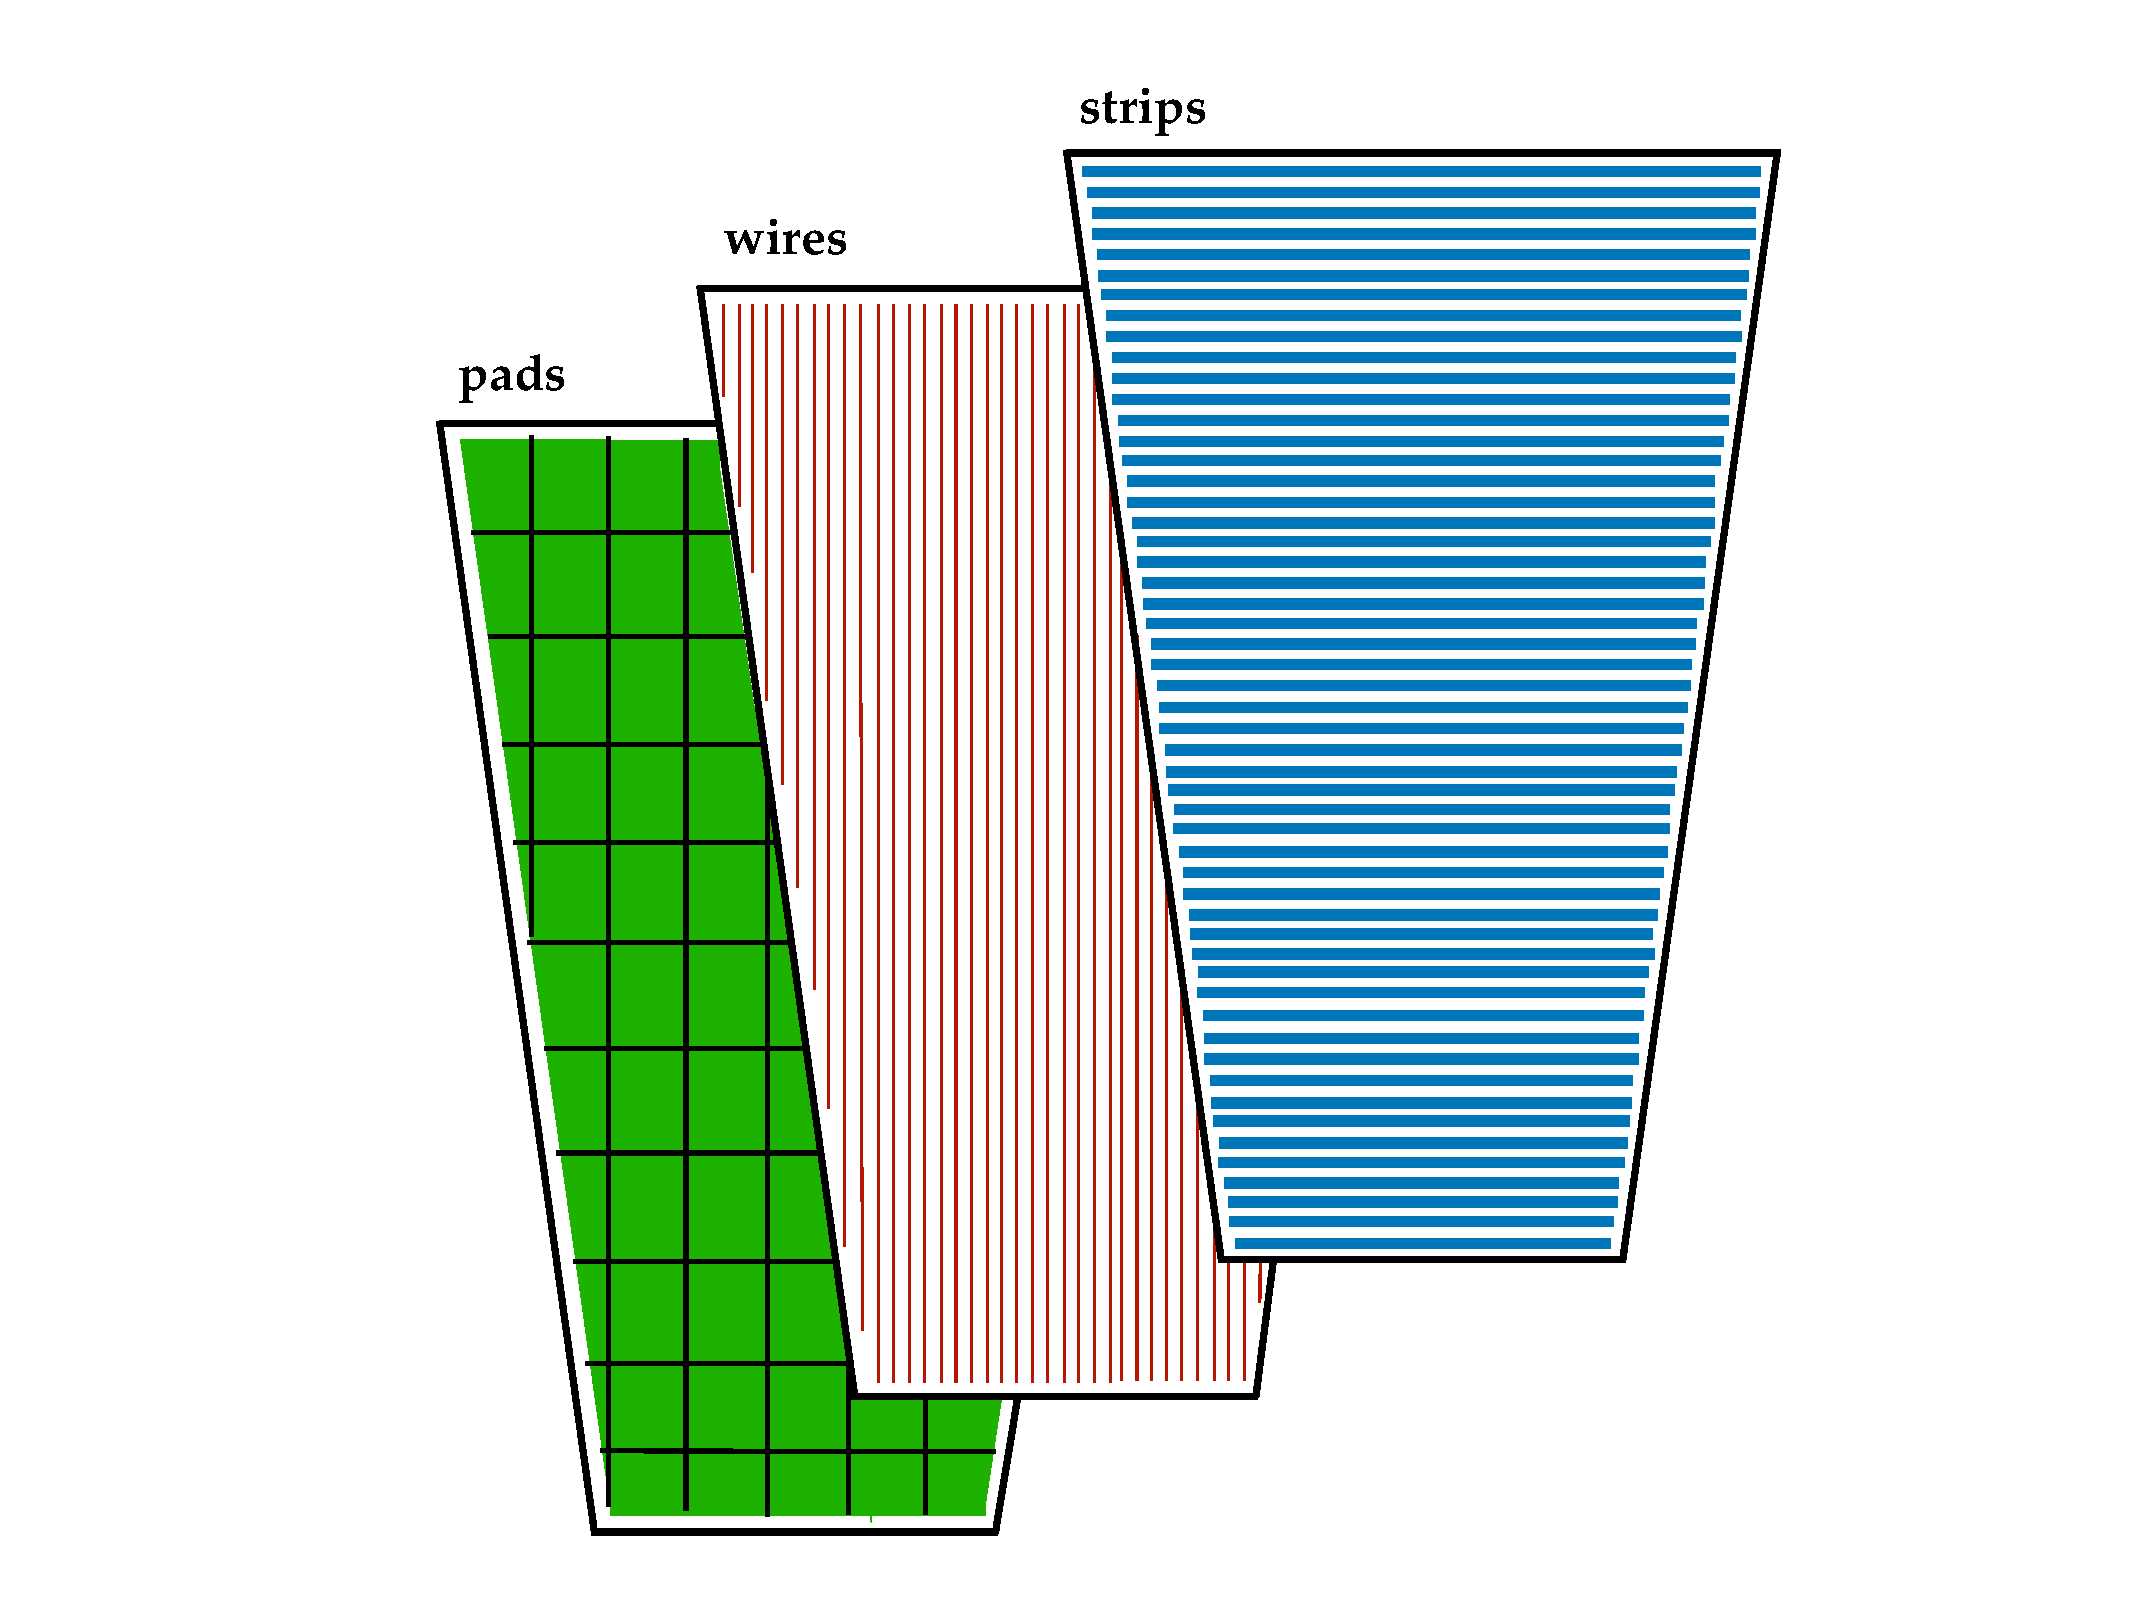
\includegraphics[width=0.45\textwidth]{figures/nsw/stgc_layer_cartoonPDF}
        \caption{
            \textbf{\textit{Left}}: Graphical representation of the internal structure of an
                sTGC detector.
                The passage of a traversing MIP (black line) induces signals on the anode wires, readout pads,
                and strips behind the resistive cathode planes as a result of the drifting of ionisation
                charges and their subsequent multiplication (in red).
            \textbf{\textit{Right}}: Illustration of the geometry of the sTGC pads, wires, and strips and their
                relative layout in a single sTGC layer.
                The strips (blue) are along $\phi$ and provide the measurement of the precision momentum coordinate
                in the particle bending plane.
                The wires are along $r$ and provide measurements sensitive to $\phi$.
                The pads provide information necessary for building trigger coincidences between
                the layers of an sTGC quadruplet and determine which subset of wires and strips will
                subsequently be readout upon a Level-1 trigger accept.
                The drawing is not to scale and does not illustrate the actual segmentation
                of the readout components in a given layer, only their relative orientation.
        }
        \label{fig:stgc_drawing}
    \end{center}
\end{figure}

\FloatBarrier

%%%%%%%%%%%%%%%%%%%%%%%%%%%%%%%%%%%%%%%%%%%%%%%%%%%%%%%%%%%%%%%%%%%%%%%
% NSW ELX
%%%%%%%%%%%%%%%%%%%%%%%%%%%%%%%%%%%%%%%%%%%%%%%%%%%%%%%%%%%%%%%%%%%%%%%
\section{NSW Readout Electronics and Detector Instrumentation}
\label{sec:nsw_elx}

{\color{make it clearer that the tracking data readout of both sTGC and MM is very similar, since they
both use the VMM...?}}

To a very large extent, high-performance detectors are realised and made
possible only by their interfacing to equally high-performance readout electronics;
that is, high quality electronics enable high quality detectors.
{\color{red}{See Appendix XXX for a discussion on the general characteristics of
detector readout electronics.}}
In this section, therefore, an introduction to the frontend electronics\footnote{`Frontend' electronics
are those housed directly on the detectors themselves and are responsible for reading out the
detector signals and potentially many other responsibilities, such as calibration, configuration, and
detector controls (temperature monitoring, etc...). `Backend' electronics refer to those
not necessarily located in the experimental cavern housing the detectors but are in the nearby
service areas or on the surface (c.f. Figu:e~\ref{fig:p1}) and are dedicated, for example, to the implementation of detector trigger logic
and data decoding and event building (i.e. gathering all data from detector hits associated with a given event).}
relevant to the NSW will be given.
There is a large set of both frontend and backend electronics specifically
designed and constructed for the NSW~\cite{NSWFrontEndChristos}.
Here, though, we will focus primarily on the frontend electronics.
The NSW frontend electronics revolve around the operation of a family
of rather complex application specific integrated circuits (ASICs),
each targetting a specific (set of) purpose(s) related to data-acquisition or
constructing trigger primitives:
%including a family of application specific integrated circuits (ASICs):

\begin{description}
    \item[] \textbf{VMM}~\cite{VMM1GDG,VMMASIC,VMM3George} Frontend readout ASIC used for precision and fast trigger data signal collection in both MM and sTGC detectors
    \item[] \textbf{ROC}~\cite{NSWTDR,NSWFrontEndChristos} `ReadOut Controller' ASIC, responsible for buffering and aggregating precision data from the VMM
    \item[] \textbf{TDS}~\cite{TDS} `Trigger Data Serialiser' ASIC, processes trigger signals from VMMs on the sTGC detectors and prepares trigger primitives for the NSW Level-1 muon trigger logic
    \item[] \textbf{ART}~\cite{NSWTDR,ARTASIC} 'Address in Real Time' ASIC, processes trigger signals from VMMs on the MM detectors and prepares trigger primitives for the NSW Level-1 muon trigger logic
\end{description}

The VMM ASIC is the primary ASIC of the NSW: all other ASICs listed above take as input
the outputs of the VMM and, in this respect, are secondary.
The work of the current author on the NSW frontend electronics is based almost exclusively
on the characterisation and validation of the VMM ASIC.
For these reasons, focus will be given on describing the VMM in Section~\ref{sec:vmm}.
For the interested reader, further information on the ROC, TDS, and ART ASICs is
provided in the references above.
The interface of the NSW frontend electronics to the associated detectors is dictated for the most part
by the geometry, type, and number of the detectors' readout elements (MM: strips, sTGC: strips, wires, and pads)
and foreseen space limitations in the ATLAS detector.
The work in the present thesis concerns the frontend boards related to the MM detectors.
This is mainly due to the fact that the VMM was initially conceptualised as a frontend ASIC specialised
for MPGD detectors and its initial prototypes were studied under this context by the RD51 collaboration
at CERN which is devoted to the development of MPGD technologies, such as the MM detectors.\footnote{For more information
on the RD51 collaboration, visit their homepage: \url{http://rd51-public.web.cern.ch/rd51-public/}.}
In Section~\ref{sec:nsw_boards}, then, a description of the relevant front-end boards used in the
study, validation, and integration of the VMM ASIC, as well as those that will be used in
the MM detectors of the NSW, will be given.
The analgogous VMM-based frontend boards for the sTGC detectors are objectively more complicated than those
of the MM detectors for purely technical and uninteresting reasons.
Their description can be found elsewhere~\cite{NSWTDR}.
{\color{red}{Maybe change how I describe why I am focused on MM detectors etc...}}

\subsection{The VMM ASIC}
\label{sec:vmm}

The VMM is a custom ASIC that can be used in a variety of charge-interpolated tracking
detectors.
There have been several iterations of the VMM over the years, starting with the VMM1~\cite{VMM1GDG} and
moving up to the VMM3~\cite{VMMASIC,VMM3George}.
An illustration of the evolution of complexity of the VMM ASIC is shown in Figure~\ref{fig:vmms_silicon}.
The VMM1 was a purely analog readout ASIC considered to be a prototype of the initial VMM functionalities.
The VMM2 was an extensive upgrade of the VMM1, adding the necessary digital logic and functional blocks
required for the NSW detectors.
The VMM3 is the final version of the ASIC\footnote{In actuality, there have been two versions of the
VMM3: the VMM3 and the `VMM3a'. The VMM3a is the true final version that will be used in the NSW
and addresses issues found during the testing and validation of the first round of the VMM3 production}
providing enhanced functionality required for data taking in ATLAS
as well as addressing bugs found in the operation of the VMM2
VMM3 is the version that will be used
in the NSW once installed in ATLAS.
The VMM implements all logic using triple modular redundancy (TMR) to protect itself
from single event upsets (SEUs) that are expected to be quite common in the
harsh radiation environments in which the NSW will be situated.

The VMM is composed of 64 discrete frontend channels, each to be connected to a detector
readout element.
A block diagram illustrating the functional blocks of the VMM3 and its channels is
shown in Figure~\ref{fig:vmm3_channel}.
Each channel has a dedicated charge amplifier (`CA' in Figure~\ref{fig:vmm3_channel}) and signal
shaping functionality,
threshold discriminator, test-pulse injection capacitor with adjustable amplitude provided
by a 10-bit digital-to-analog converter (DAC), and precise signal amplitude and timing measurements digitally readout via
internal per-channel analog-to-digital converters (ADCs).
The amplitude measurement of the input pulse is digitised by a 10-bit ADC (`PDO', for `peak detector output', in Figure~\ref{fig:vmm3_channel})
and the timing estimation of the signal pulse's peak is digitised by an 8-bit ADC (`TDO', for `time detector output', in Figure~\ref{fig:vmm3_channel}).
The digitised output of these amplitude and timing measurements are calculated by these
internal ADCs within 200\,ns and stored in internal buffers of the VMM.
The buffered data is stored until selected for readout by another ASIC housed on the same frontend
board as the VMM, the ROC, based on the buffered data's bunch crossing.
The PDO and TDO data are those used in the precision hit reconstruction in the detectors.
The hit timing information provided by the TDO is critical only for the MM detectors which
rely primarily on the $\mu$-TPC hit reconstruction method, as illustrated in Figure~\ref{fig:mm_tpc_hit_loc} (right).
For the sTGC, the accurate timing information is not required for precision tracking and,
to increase readout bandwidth, the timing information will likely not be serialised
in the data output from the sTGC frontend electronics.
%{\color{red}{For the precision hit reconstruction, the timing information is critical only for the MM
%detectors which rely on the $\mu$-TPC hit reconstruction method which requires
%precision time measurements for building the tracklets within the drift region of the
%MM detector. For the sTGC the accurate timing information is not required
%for precision tracking and, to increase readout bandwidth, the timing information will not be
%serialised.}}

In addition to the precision data useful for reconstructing high-level muon tracks provided by
the PDO and TDO measurements, the VMM can also operate at a faster mode used for
providing data needed for the building of trigger primitives.
In the trigger mode referred to as the `Address-in-Real-Time' (ART) mode,
the VMM outputs the \textit{first} channel address (i.e. MM strip number) on which
an above-threshold peak was detected.
An alternative trigger mode relies on the VMM's ability to perform a fast digitisation of
the signal pulse amplitude using a 6-bit ADC, providing a coarse but rapid measurement
of the signal amplitude.
Additionally, the VMM can output fast timing signals, such as a flag indicating a signal over threshold (`Time-Over-Threshold', or TOT as in Figure~\ref{fig:vmm3_channel}).
The ART trigger scheme is used for the MM trigger primitives and the combination
of the coarse 6-bit amplitude and fast-timing signals is used for building the
sTGC trigger primitives.

One of the powers of the VMM is its highly configurable nature.
This, of course, makes the ASIC quite complex in terms of its design but is
advantageous in terms of its range usefulness.
Some of the main configurable items are the peaking (integration) time of the signal shaper
(25, 50, 100, and 200\,ns), adjustable thresholds per-VMM configured by an on-VMM
10-bit (DAC),
adjustable channel gains (0.5, 1, 3, 4.5, 6, 9, 12, and 16\,mV/fC),
time-to-amplitude conversion (TAC) ramp time (60, 100, 350, and 650\,ns) relevant for the timing measurements,
and channel threshold trimmers provided by 5-bit DACs that adjust each channel's individual
threshold around the globally-configured (per-VMM) threshold.
The VMM input can also be configured to handle either positive or negative input
signals.
This latter fact is necessary for the NSW, in which the sTGC and MM detectors
will induce signals of opposite polarity on their readout elements.\footnote{The MM strips and
sTGC wires produce signals of opposite polarity as the sTGC strips and pads.}

\begin{figure}[!htb]
    \begin{center}
        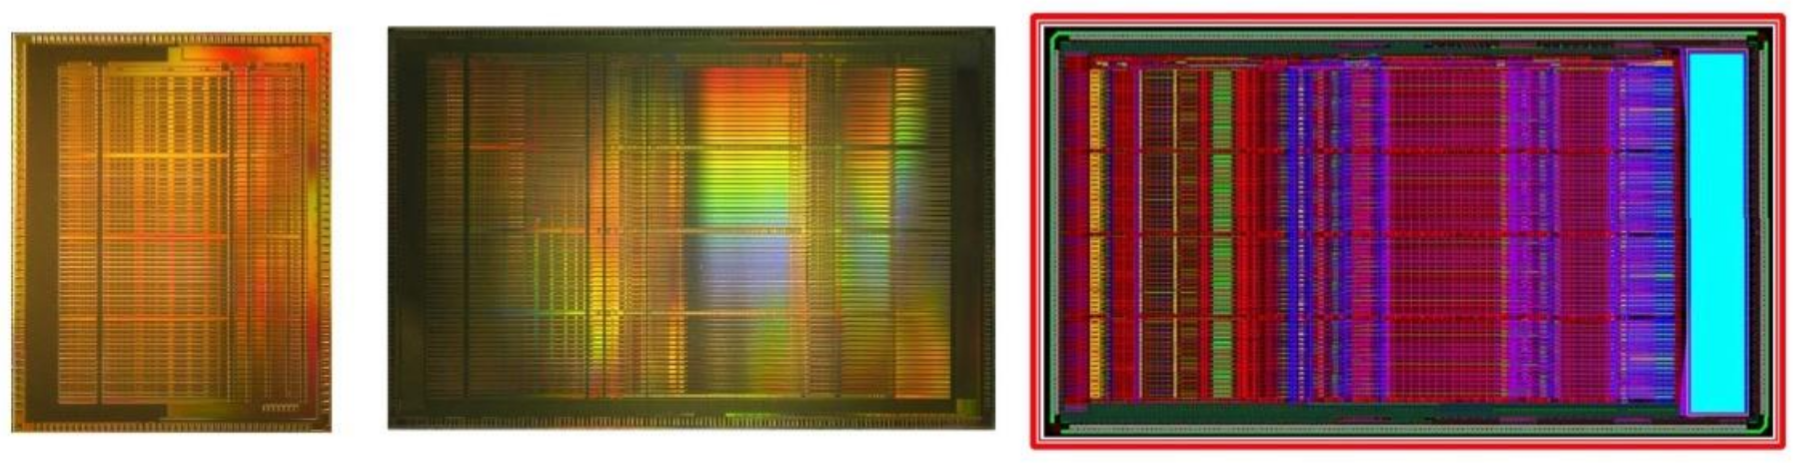
\includegraphics[width=0.8\textwidth]{figures/nsw/vmm/vmms_silicon}
        \caption{
            Evolution of the VMM ASIC.
            Shown are the silicon dies or routing of the the VMM1 (\textbf{\textit{left}}), to the VMM2 (\textbf{\textit{middle}}), and 
            the VMM3 (\textbf{\textit{right}}), the final version that will be used in the NSW.
            The VMM1 has an area of 50\,mm$^2$ with $\approx 500$\,k MOSFETs, the VMM2 area is 115\,mm$^2$ with $>5$\,M MOSFETs,
            and the VMM3 area is 130\,mm$^2$ with $>6$\,M MOSFETs.\protect\footnotemark%
        }
        \label{fig:vmms_silicon}
    \end{center}
\end{figure}
\footnotetext{`MOSFET' stands for metal-oxide-semiconductor field-effect  transistor', the most widely used transistor in digital and analog electronics.}

\begin{figure}[!htb]
    \begin{center}
        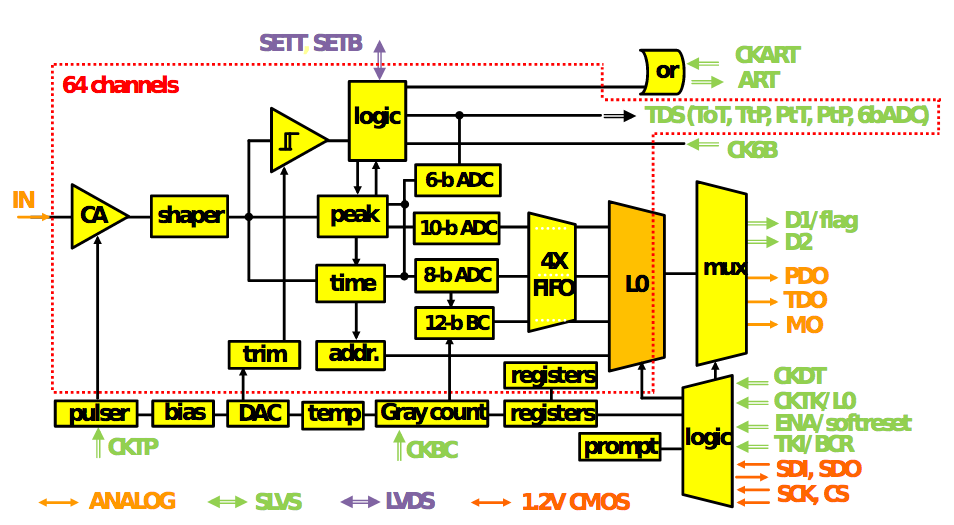
\includegraphics[width=0.8\textwidth]{figures/nsw/vmm/vmm3_channel}
        \caption{
            Architecture of the VMM3.
            The items contained within the dotted red line are repeated
            for each of the 64 channels of the VMM.
        }
        \label{fig:vmm3_channel}
    \end{center}
\end{figure}

\subsection{Frontend-electronics Boards for the NSW}
\label{sec:nsw_boards}

There have been two classes of frontend boards encountered
throughout the work on the NSW electronics represented in this thesis.
The first class relates to a type of frontend board that is not specific to the NSW
but which houses one (or several) VMM ASICs.
The second class relates to prototype frontend boards following the design to be used
in the NSW to readout the MM detectors, the so-called MMFE8 frontend board.
Figure~\ref{fig:frontend_boards} provides pictures of these two classes of frontend
boards with relevant parts indicated.

The general purpose frontend boards, such as the GPVMM in Figure~\ref{fig:frontend_boards}, are those used primarily for the direct study
and characterisation of the VMM ASIC.
The prototype MMFE8 frontend boards allow for a more realistic interface to the MM
detectors to be studied as well as for the overall design and layout of the hardware components on the
boards themselves to be studied and optimised.
One such optimisation was the placement of the DC-to-DC converters used for the on-board power distribution.\footnote{In the
final MMFE8 prototype frontend boards, and in those to be used in the NSW,
the DC-to-DC converters are packaged in the so-called FEAST ASIC developed by CERN.
Further information at \url{https://project-dcdc.web.cern.ch/project-dcdc/Default.html}}
DC-to-DC converters are potential sources of electronic noise and stray electromagnetic fields as a result of
their high switching frequencies.
When placed directly on the frontend boards, their nearness to the noise-sensitive readout
elements means that the matter of their placement and shielding needs to be handled carefully.

The types of boards discussed here have allowed for the study of the VMM ASIC both on- and off-detector,
where in the latter case prototype MM detectors were used ({\color{red}{More to say in Section XXX}}).
Over the timespan of the present thesis, many iterations of each type of frontend board
were encountered, with subsequent iterations adapting to the evolution of the VMM, for example (Figure~\ref{fig:vmms_silicon}).
In addition to housing the VMM ASIC, the frontend boards house a
\textsc{Xilinx} field-programmable gate array (FPGA). 
One of the main purposes of the FPGA is to aggregate the data being output from the VMM
and prepare it for being sent off-board via standard network protocols over Ethernet to the
backend data-acquisition system ({\color{red}{Section XXX}}).
Additionally, the FPGA responds to commands and requests submitted by users via the software
interface ({\color{red}{Section XXX}}).
Such commands may have as endpoint the FPGA itself or they may require the FPGA to forward
them to the VMM ASIC.
%may have as end and either adjusts its own configuration parameters or
%forwards the commands to the VMM such that it itself may respond.

The GPVMM board has a simple connector designed in such a way that lends itself to
be easily adapted to many types of detectors in labs and teststands.
The MMFE8 board, both the prototypes and those to be used in the NSW, use a ZEBRA\footnote{More information
on ZEBRA-type connectors can be found online at \url{https://en.wikipedia.org/wiki/Elastomeric_connector}} elastomeric
connector that allows for a seamless interconnect between the readout strips on the MM detector layers
and the VMM channel inputs.
The principle of the ZEBRA connector is illustrated in Figure~\ref{fig:zebra_connector}.
%In the final version of the MMFE8 frontend board to be used for interfacing with the MM detectors,
%the Ethernet readout will be replaced b
%the role of the FPGA will be replaced by the combination of the ROC ASIC, mentioned in the previous section,
%and the CERN-provided Slow Control Adapter (SCA) ASIC~\cite{GBTASIC}

\begin{figure}[!htb]
    \begin{center}
        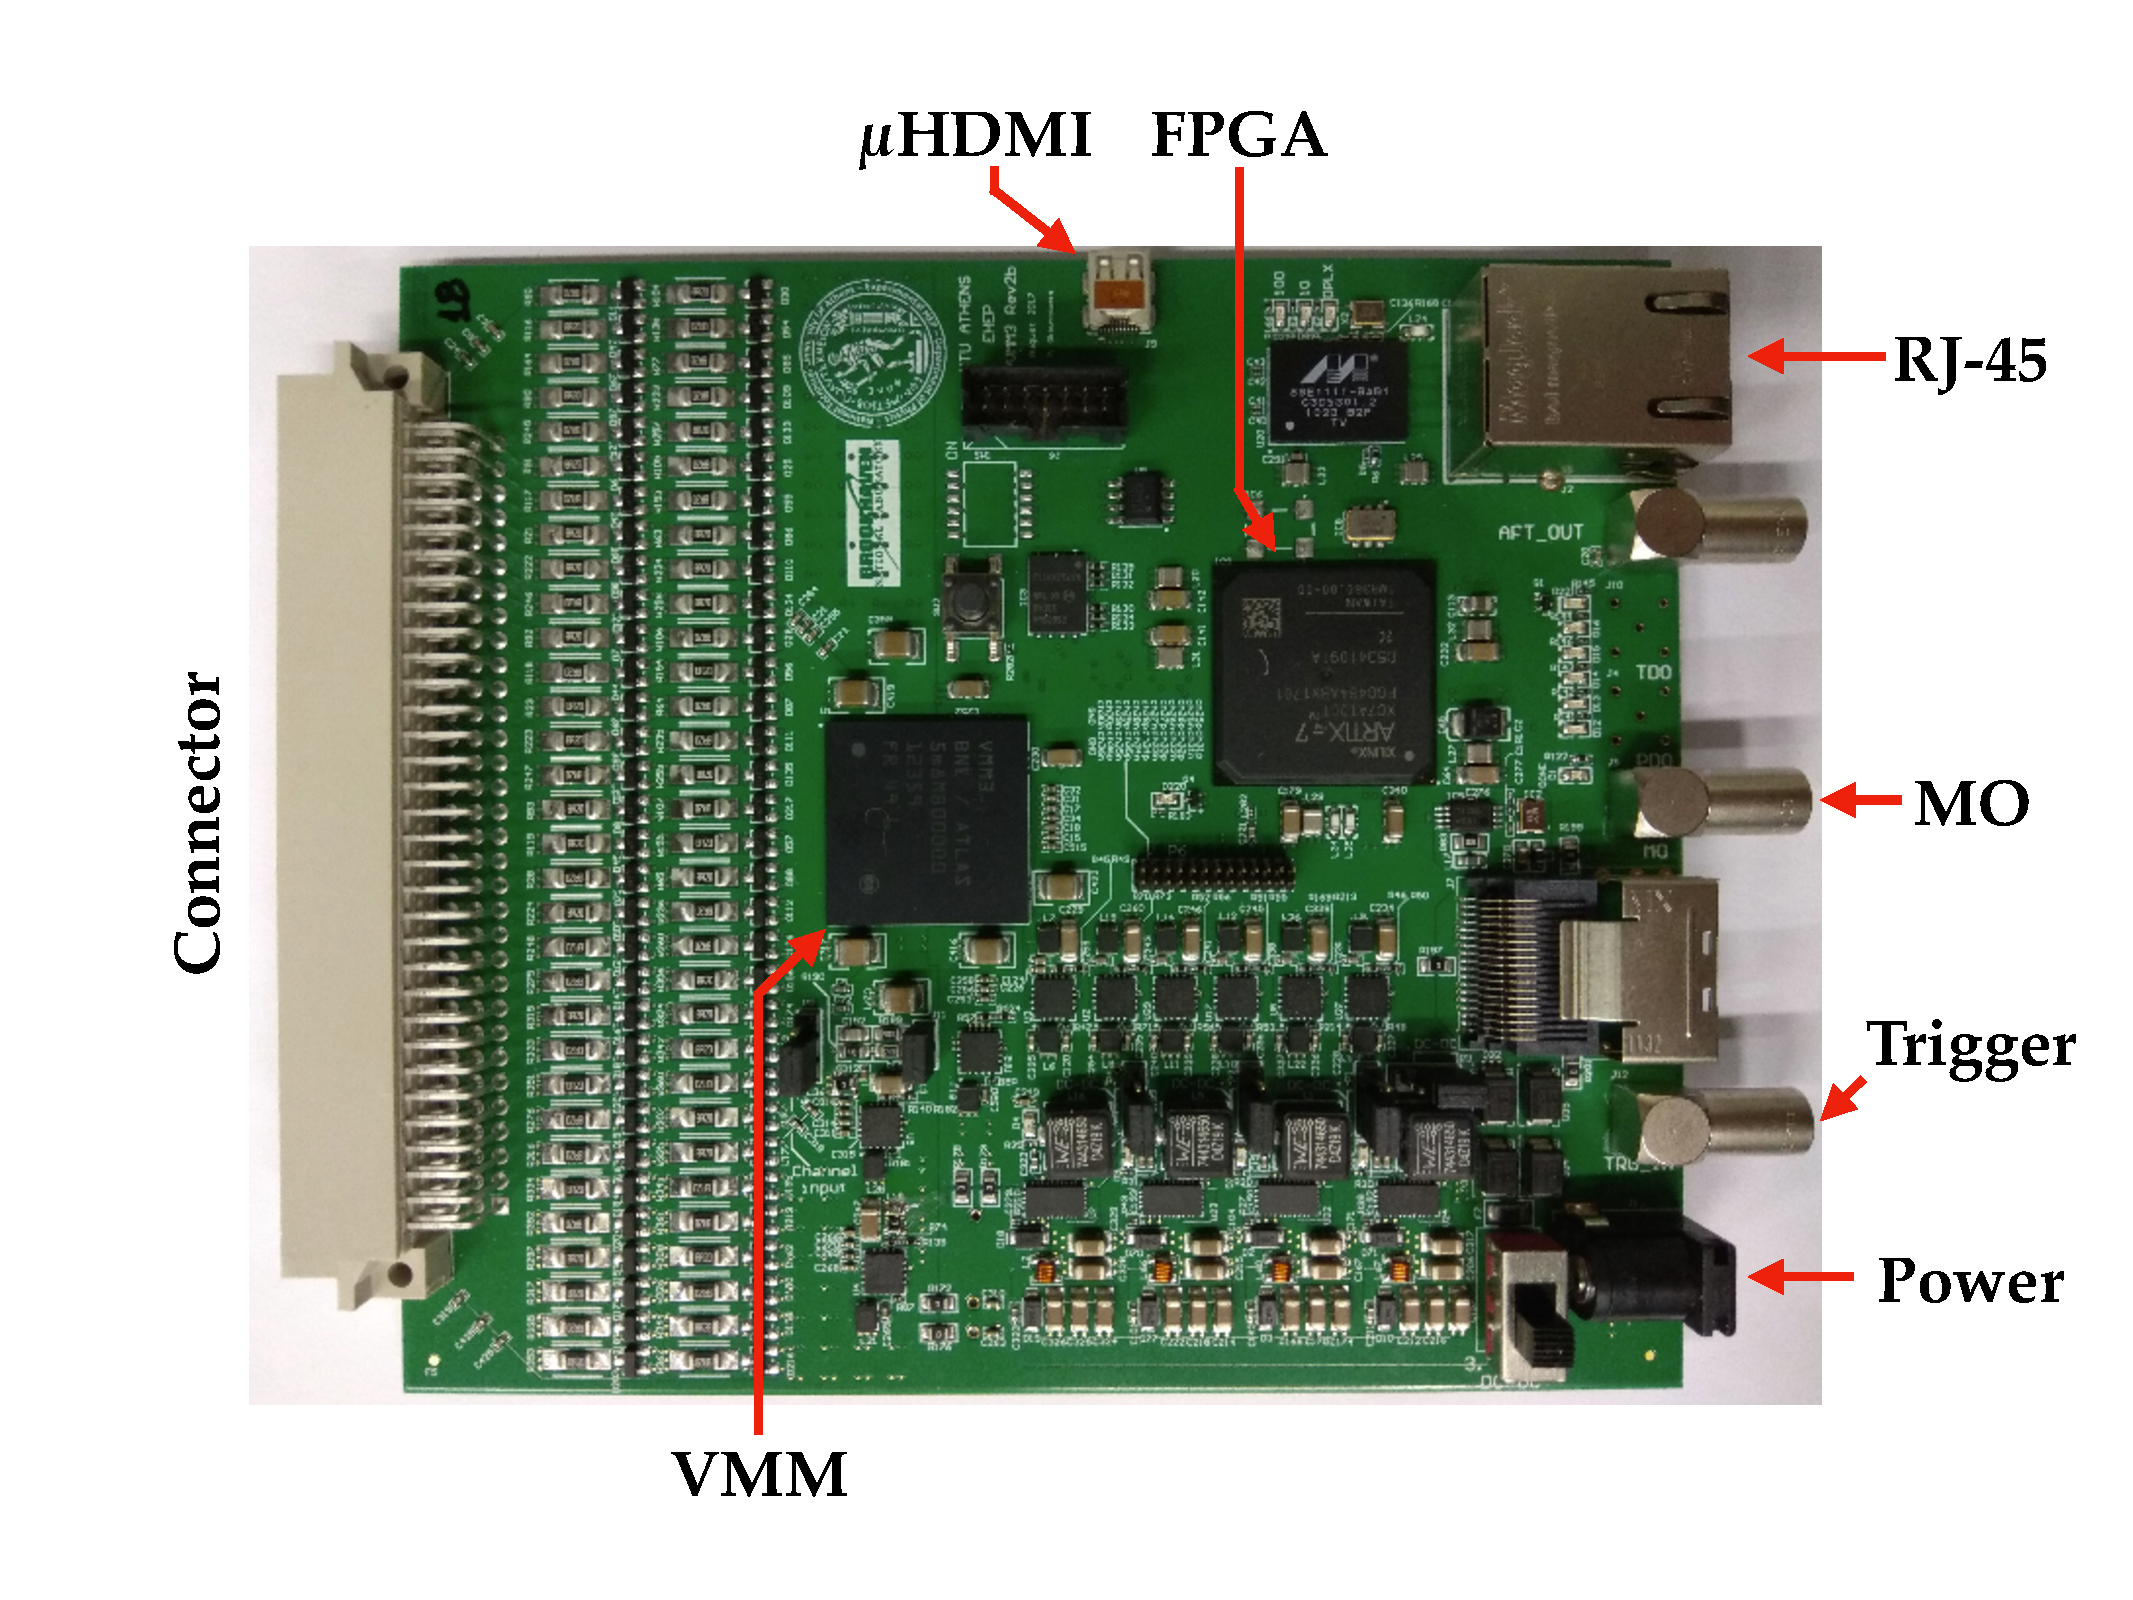
\includegraphics[width=0.8\textwidth]{figures/nsw/frontend/gpvmm_labelledPDF}
        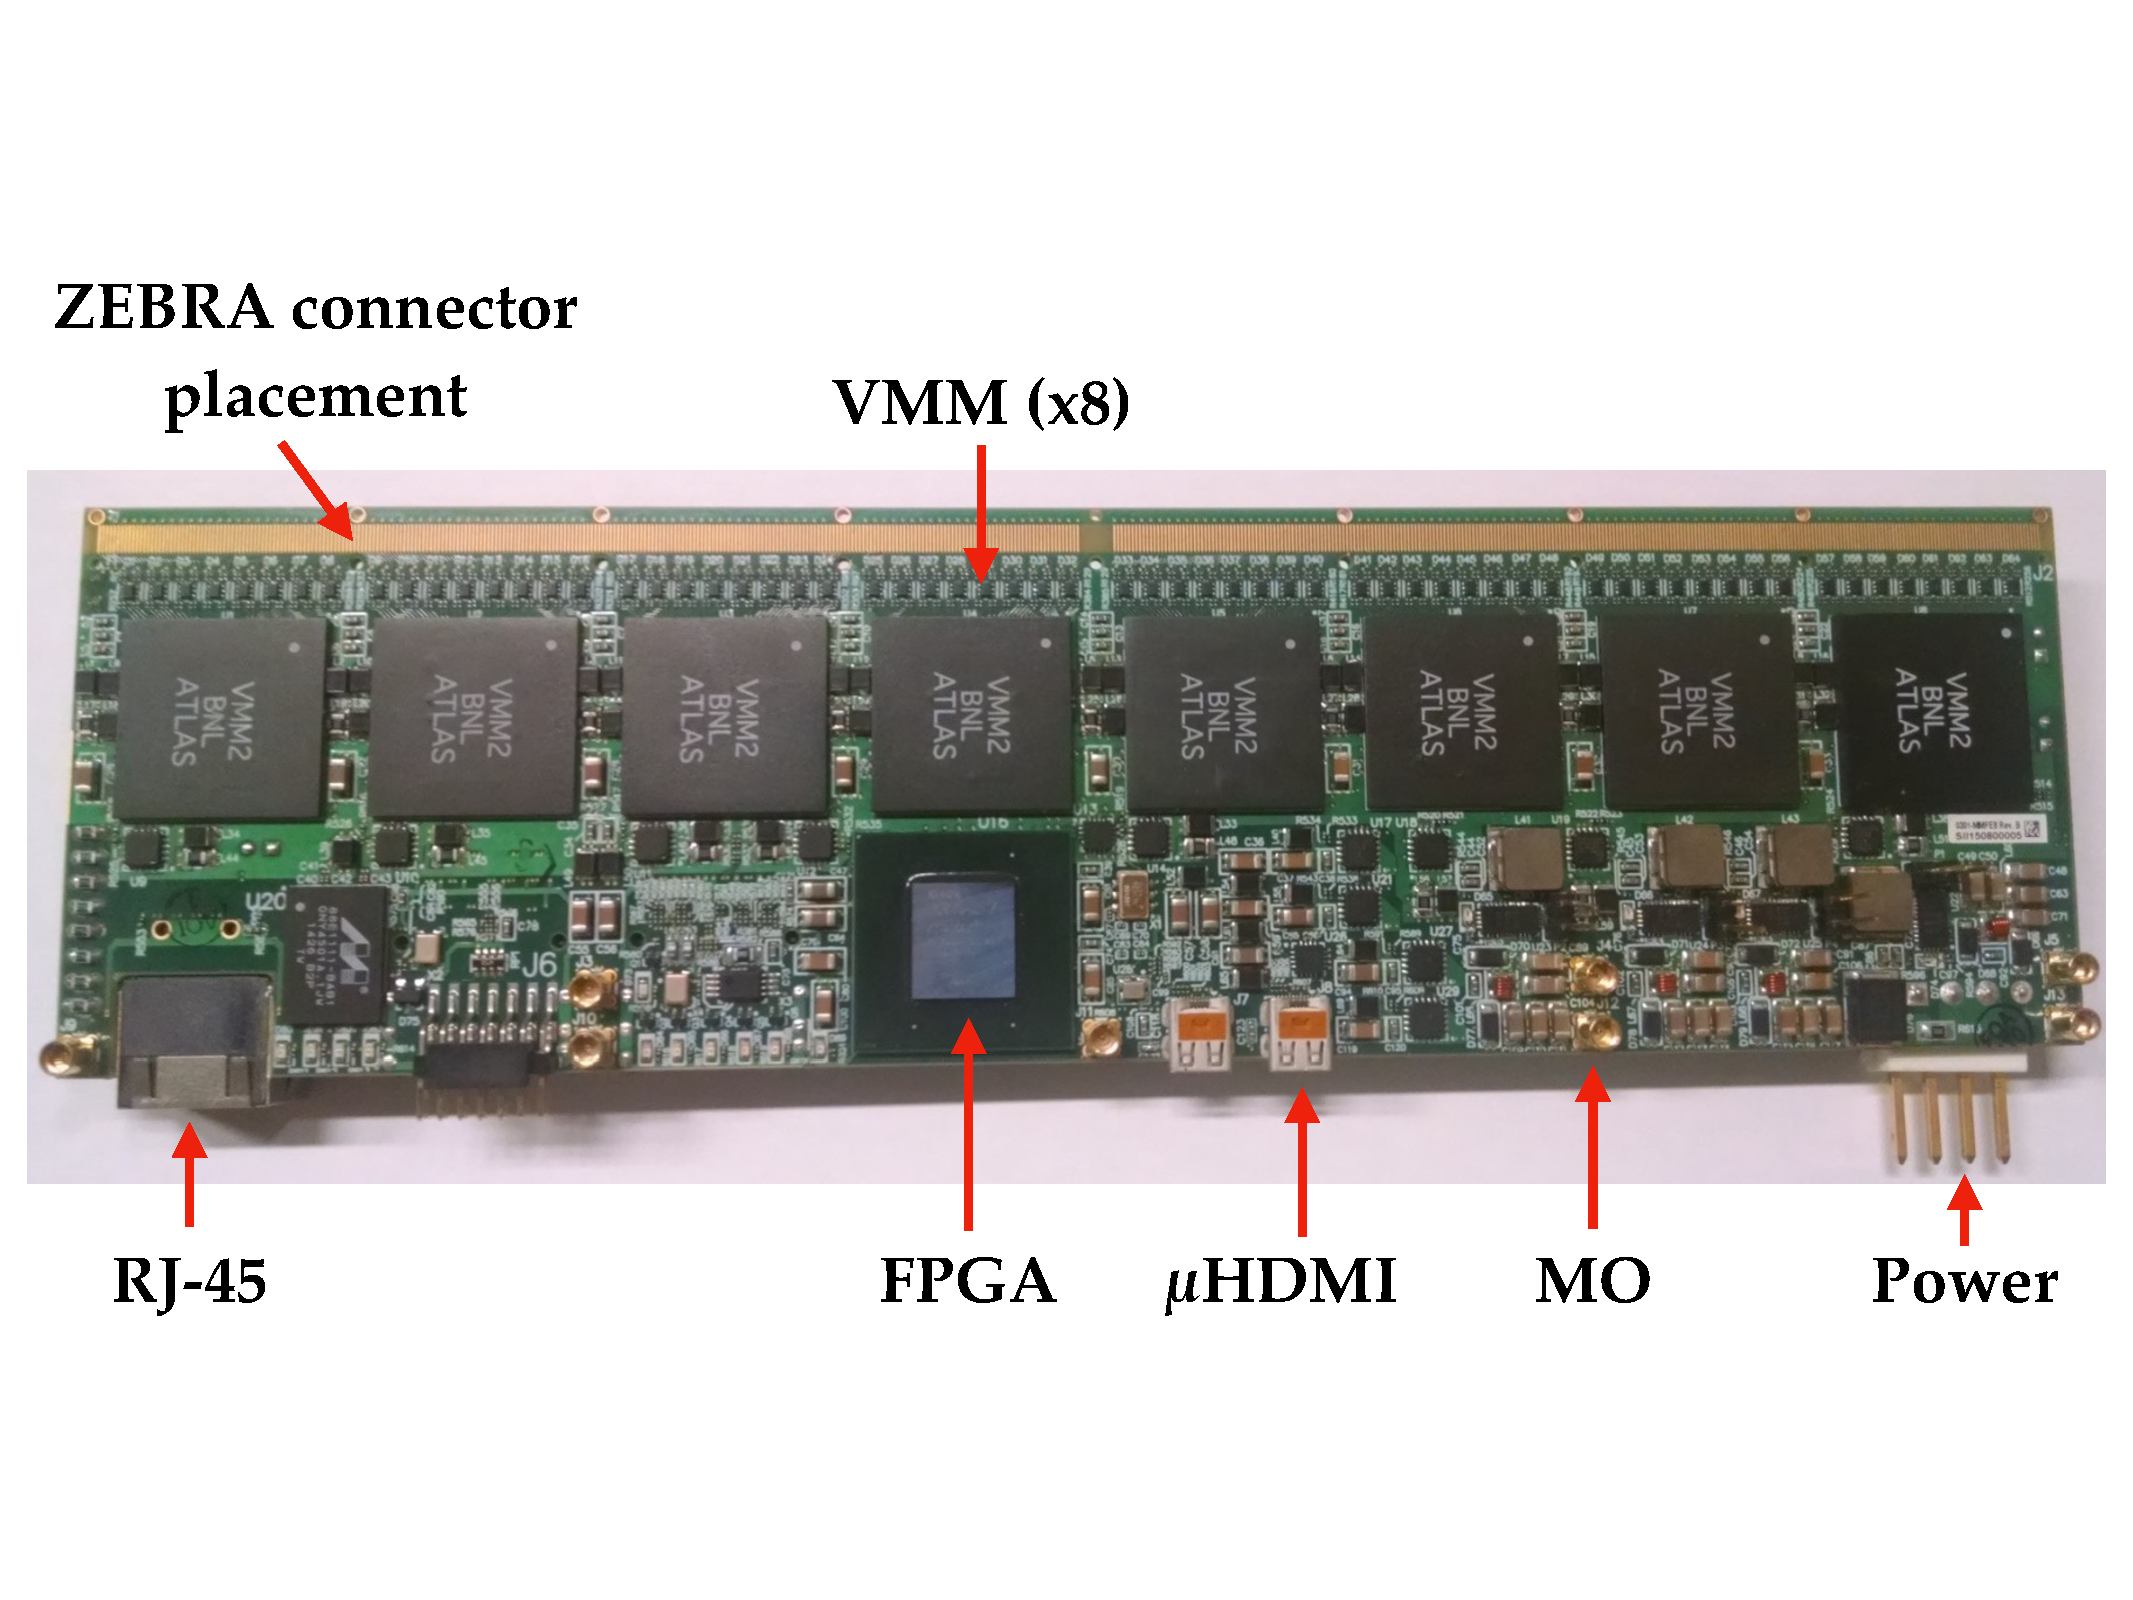
\includegraphics[width=0.8\textwidth]{figures/nsw/frontend/mmfe8_labelledPDF}
        \caption{
            Pictures of two VMM-based frontend boards. The RJ-45 connectors provide network I/O via
            standard Ethernet cables.
            The $\mu$HDMI connectors provide inputs for additional signalling purposes, such as external
            trigger signals.
            `MO' refers to the multiplexed monitoring output of the VMM (see Figure~\ref{fig:vmm3_channel}), which samples the analog
            signals internal to the VMM, such as the shaped input signals, prior to their digitisation.
            \textbf{\textit{Top}}: General purpose VMM (GPVMM) board housing a single VMM ASIC.
            The MO and trigger I/O are provided by LEMO connectors.
            \textbf{\textit{Bottom}}: Prototype MMFE8 board with its 8 VMM ASICs.
            The ZEBRA connector used for the MM detectors is described in the text.
            On this board the MO output is accessible primarily by the use of a oscilloscope probe.
        }
        \label{fig:frontend_boards}
    \end{center}
\end{figure}

\begin{figure}[!htb]
    \begin{center}
        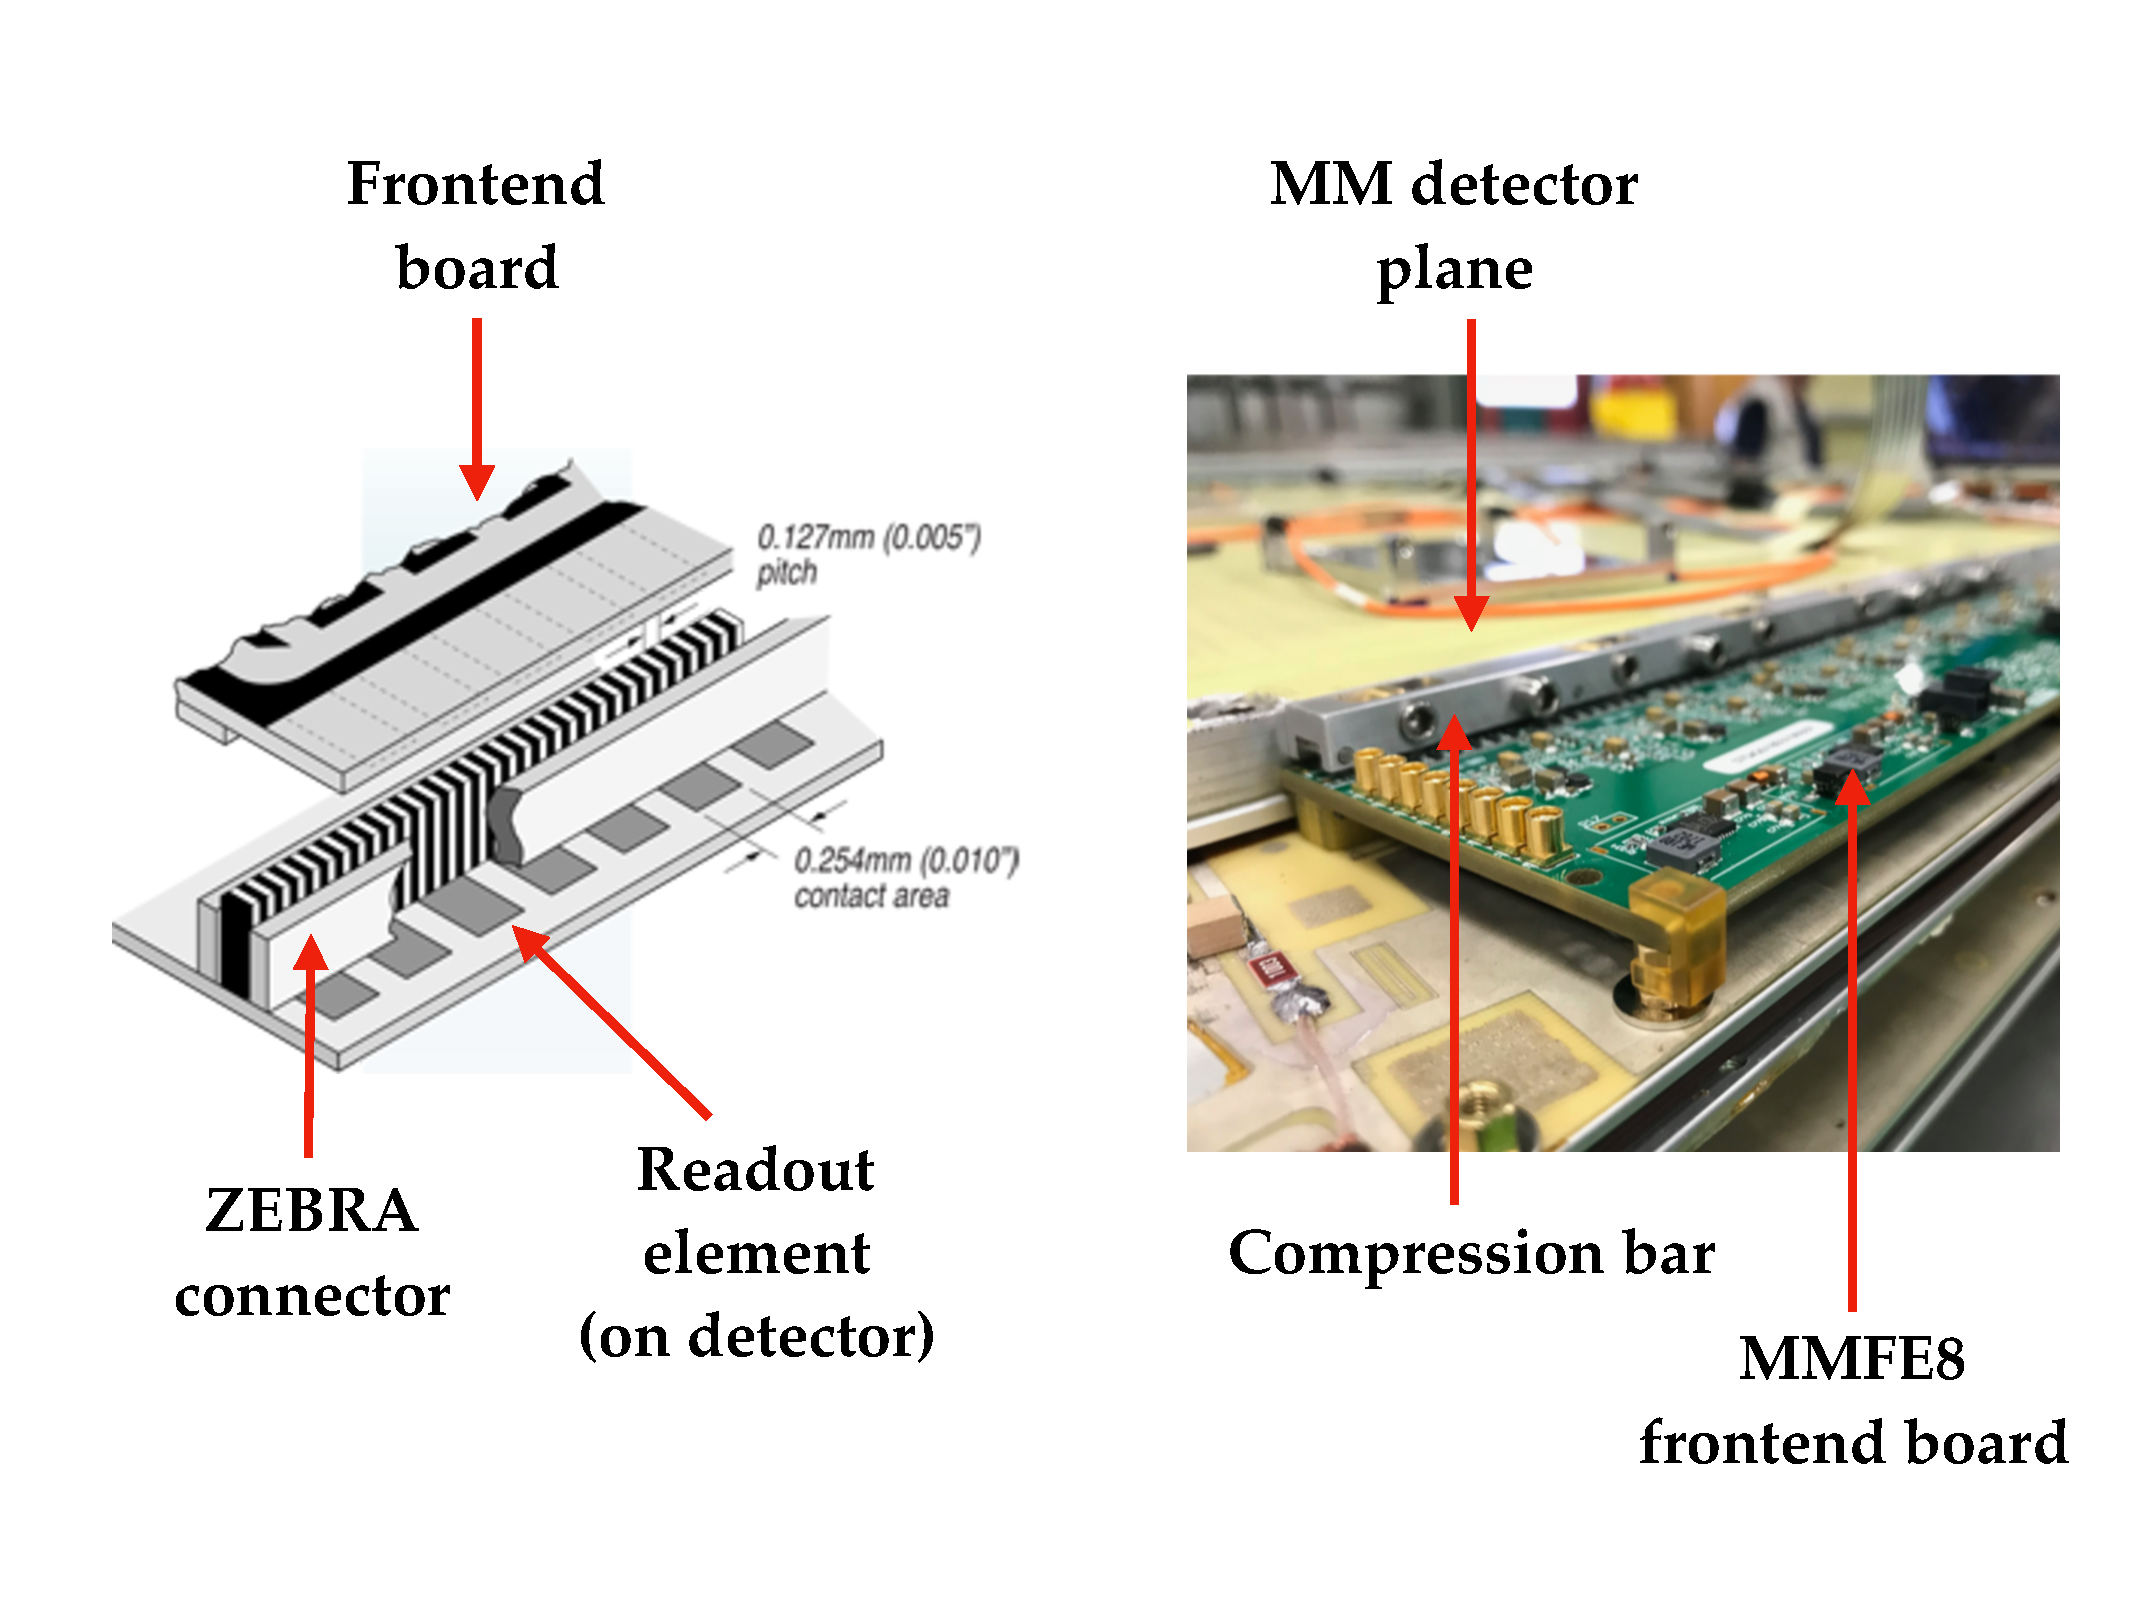
\includegraphics[width=0.8\textwidth]{figures/nsw/frontend/zebra_connector_illustratedPDF}
        \caption{
            \textbf{\textit{Left}}: Illustration of the ZEBRA connector concept.
                The ZEBRA connector is composed of a high density of alternating conductive (white) and non-conductive (black) layers
                that make contact with the detector readout elements on bottom and frontend board sensing elements
                on top.
            \textbf{\textit{Right}}: Picture of the ZEBRA connector being used with an MMFE8 frontend board
                on a full-scale MM detector.
                When interfaced to the MM detector, the MMFE8 frontend board is situated such that the VMMs are downward facing and
                are not therefore visible as pictured.
                The connection of the ZEBRA connector is realised via the tightening of a compression bar mounted on the MM detector chamber.
                The resulting
                downward pressure forces the ZEBRA connector to be securely sandwiched between
                the readout elements of the MM detector and VMM channel inputs located on the frontend board, bringing them in direct electrical contact.
        }
        \label{fig:zebra_connector}
    \end{center}
\end{figure}

The NSW frontend boards are interfaced directly to the detectors.
Both the GPVMM-type and MMFE8 frontend boards have been used on small prototype MM detectors, with
active area of $10\times10$\,cm$^2$.
A picture of an MMFE8 connected to such a detector is shown in Figure~\ref{fig:mmfe8_t2}.
On the full-scale MM detectors to be used in the NSW, the frontend boards are situated along the edge
of each detector layer in a given multilayer.
A drawing of a complete MM quadruplet with frontend electronics boards is shown in Figure~\ref{fig:mm_quad_elx}.


\begin{figure}[!htb]
    \begin{center}
        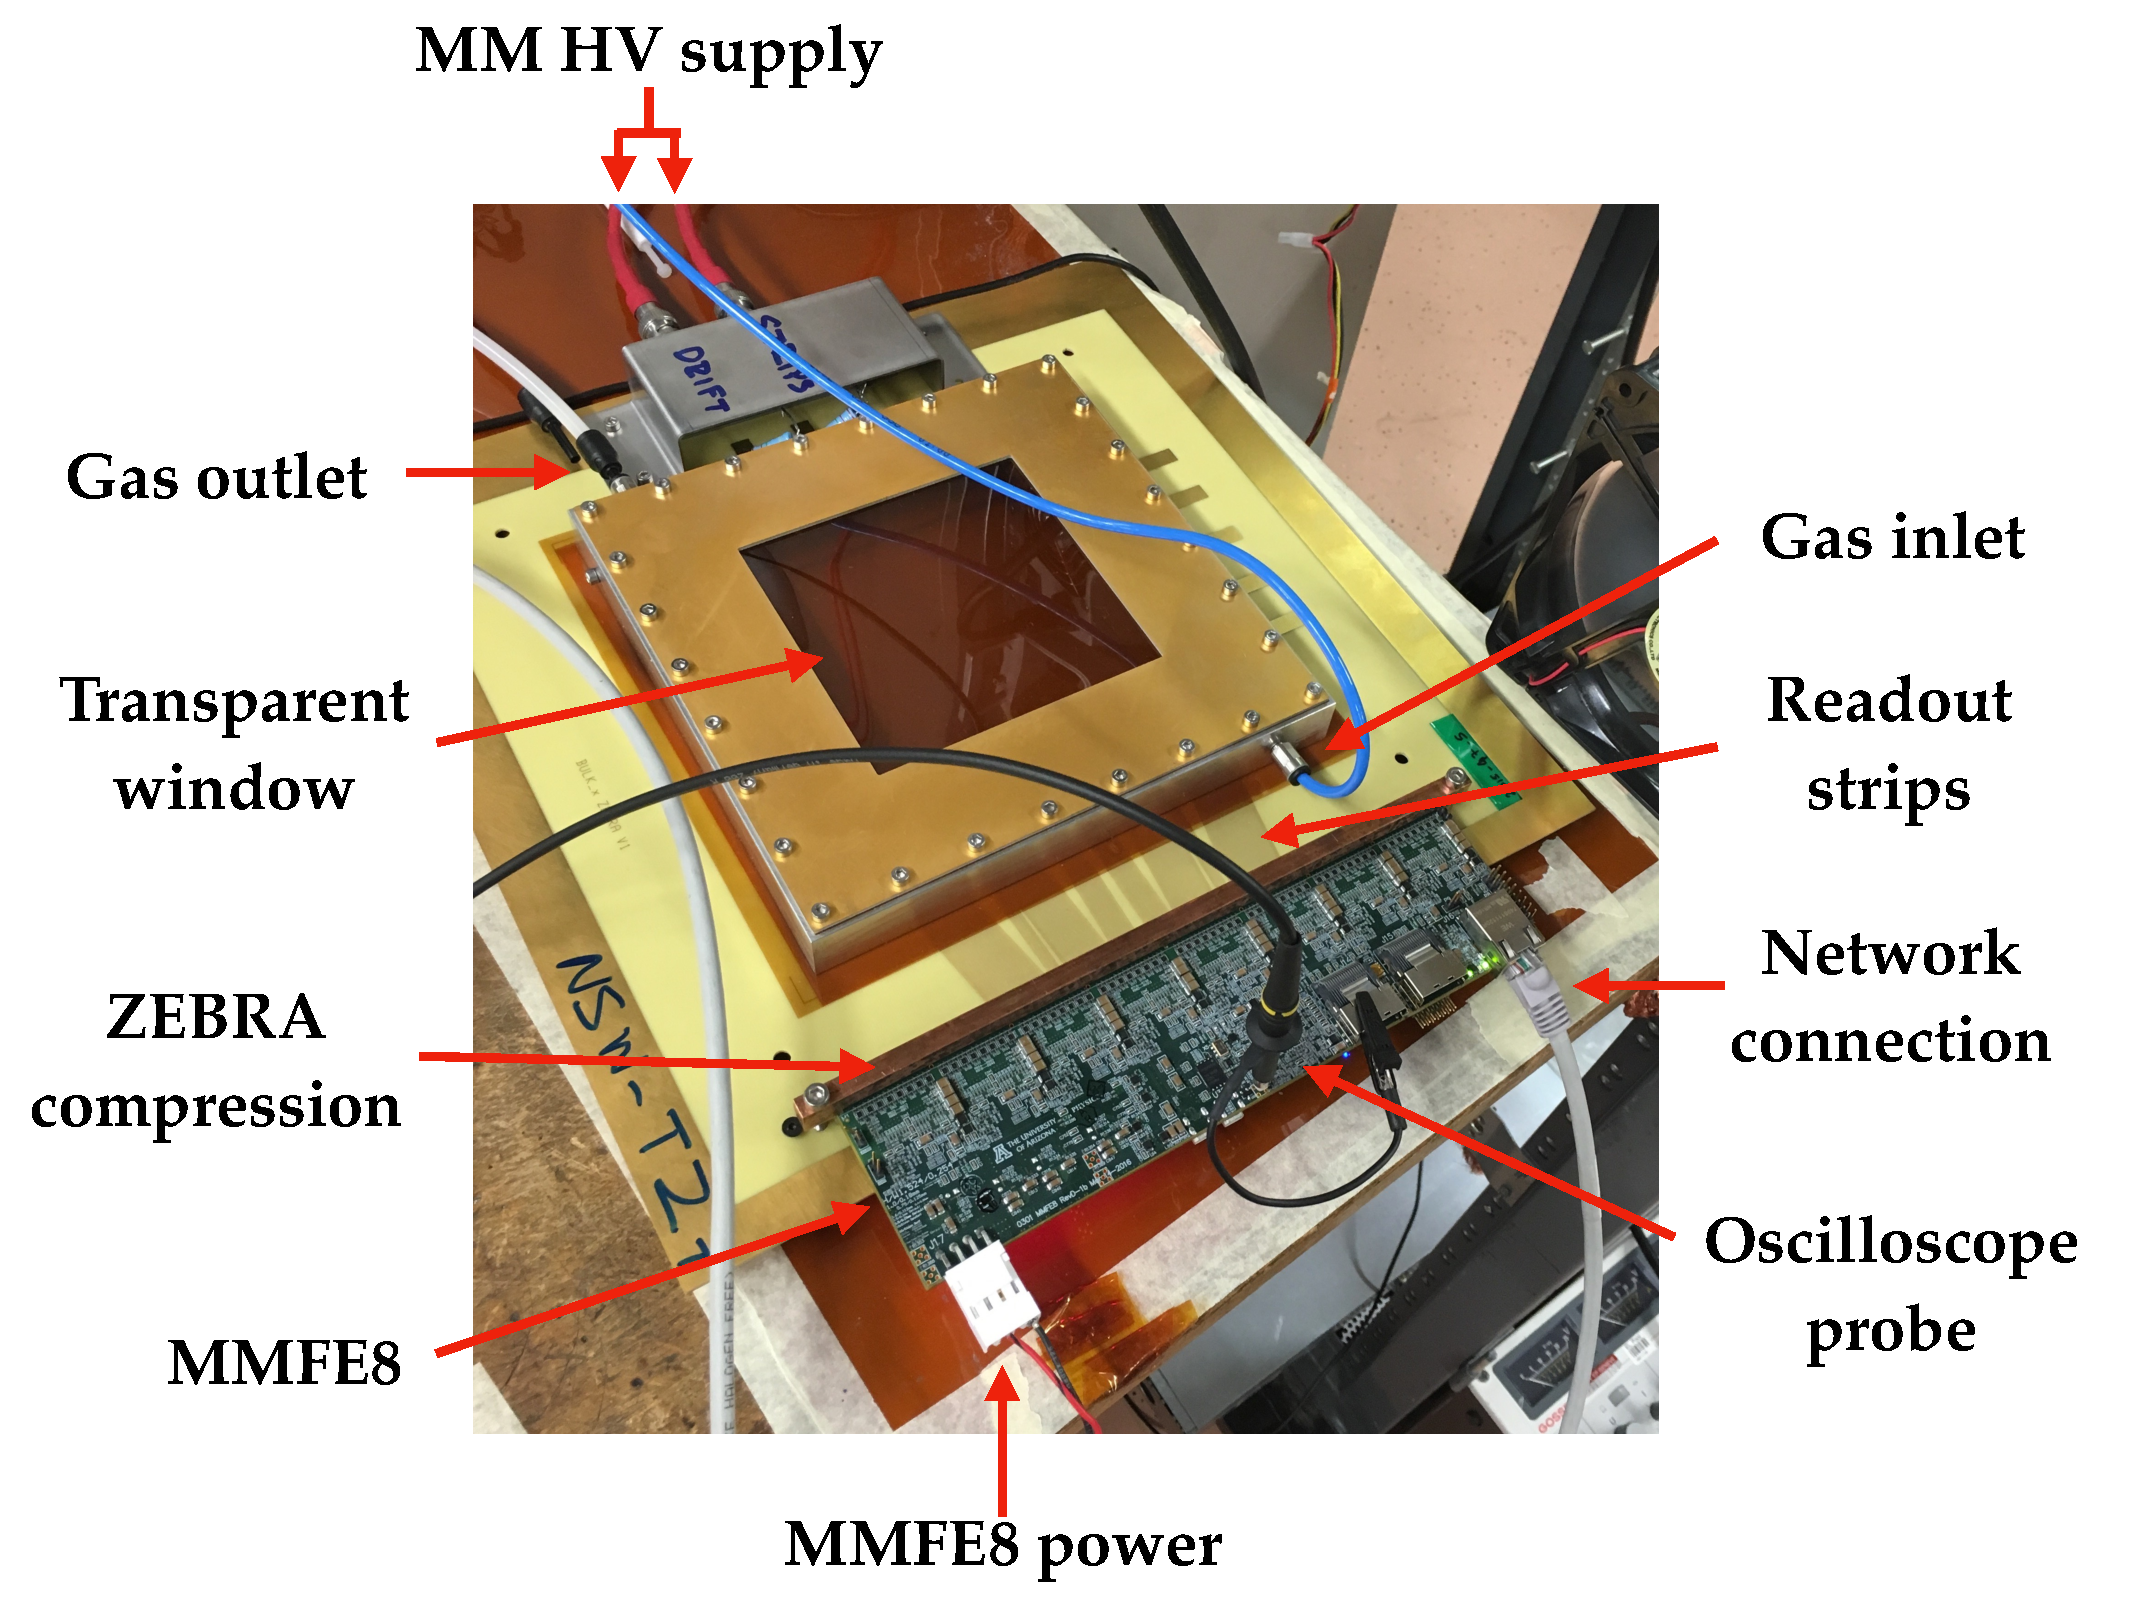
\includegraphics[width=0.75\textwidth]{figures/nsw/frontend/mmfe8_t2_labelledPDF}
        \caption{
        }
        \label{fig:mmfe8_t2}
    \end{center}
\end{figure}

\begin{figure}[!htb]
    \begin{center}
        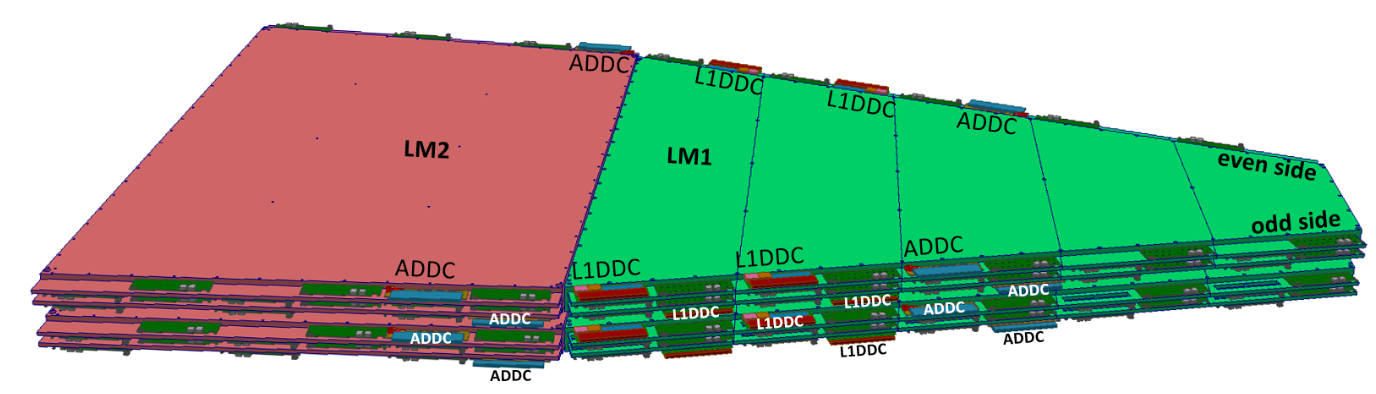
\includegraphics[width=0.8\textwidth]{figures/nsw/frontend/mm_quad_elx}
        \caption{
            {\color{red}{Explain how the frontend boards are situated on the NSW chambers}}
        }
        \label{fig:mm_quad_elx}
    \end{center}
\end{figure}

\FloatBarrier

%%%%%%%%%%%%%%%%%%%%%%%%%%%%%%%%%%%%%%%%%%%%%%%%%%%%%%%%%%%%%%%%%%%%%%%
% VRS
%%%%%%%%%%%%%%%%%%%%%%%%%%%%%%%%%%%%%%%%%%%%%%%%%%%%%%%%%%%%%%%%%%%%%%%
\section{Development of Configuration, Data-acquisition, and Calibration Software for the Validation of the NSW Frontend}
\label{sec:nsw_vrs}

To facilitate the testing and readout of the VMM ASIC, in view of its evolution
and the approaching installation of the NSW, a complete
configuration and data-acquisition (DAQ) system has been built.
The system, referred to as the `VMM Readout System' (VRS), consists of a flexible
firmware and software infrastructure that allows for
interfacing to frontend boards housing the VMM ASIC.

A minimal instantiation of the VRS system is illustrated in Figure~\ref{fig:vrs_diagram_minimal}
in which the DAQ PC, hosting the VRS software, communicates directly to a set
of frontend boards via the network.\footnote{Network communication in the VRS system is implemented following the User Datagram Protocol (UDP) network
communication protocol. Physical network connections are made using standard Ethernet cables and on-board RJ-45 connectors.}
The frontend boards need not be interfaced to a detector, as signals can be injected via
the test-pulse injection capacitors on the VMM channels.
The firmware, loaded onto the FPGA on each frontend board, implements the necessary logic for handling the network communication
between the software and the VMM ASIC.
The types of communication between the software will be described in subsequent sections, but primarily consist of configuration
commands being forwarded to either the FPGA or the VMM ASIC.
The firmware handles the logic necessary for packaging the readout data being
output by the VMMs on the associated frontend boards.
Once packaged, it then serialises the data over the network back to the DAQ PC where it can be monitored
and promptly stored on disk for later analysis.
In this minimal setup, the clock and trigger signals driving the VMM readout are generated independently
on each frontend board by the on-board FPGA.
Communication is made between the DAQ PC and a frontend board via a unique network (IP)
address associated with each frontend board that is exposed to the network by the firmware. 

The VRS system is extensible and performant enough that it may handle an arbitrary number of frontend boards
and detectors.
This is illustrated in Figure~\ref{fig:vrs_diagram} in which several detectors, with their own
set of frontend boards, are being configured and readout via the VRS system.
In this case, an external clock and trigger system send their signals to a `VRS Supervisory Board' (VSB)
which handles the synchronous transmission of these signals to the independent groups of frontend boards
located on the separate detectors.
The VSB also acts to multiplex the communication between the DAQ PC and the many grouped frontend boards:
a single network connection is made between the DAQ PC and VSB, which handles the forwarding of commands to
specific frontend boards.
This and other VSB functionalities are implemented by dedicated electronics as well as by
firmware loaded on an on-board FPGA.

The work relevant to the present thesis primarily concerns the development of the software
infrastructure of the VRS system.
In the next sections aspects of the VRS software will be introduced and described.

\begin{figure}[!htb]
    \begin{center}
        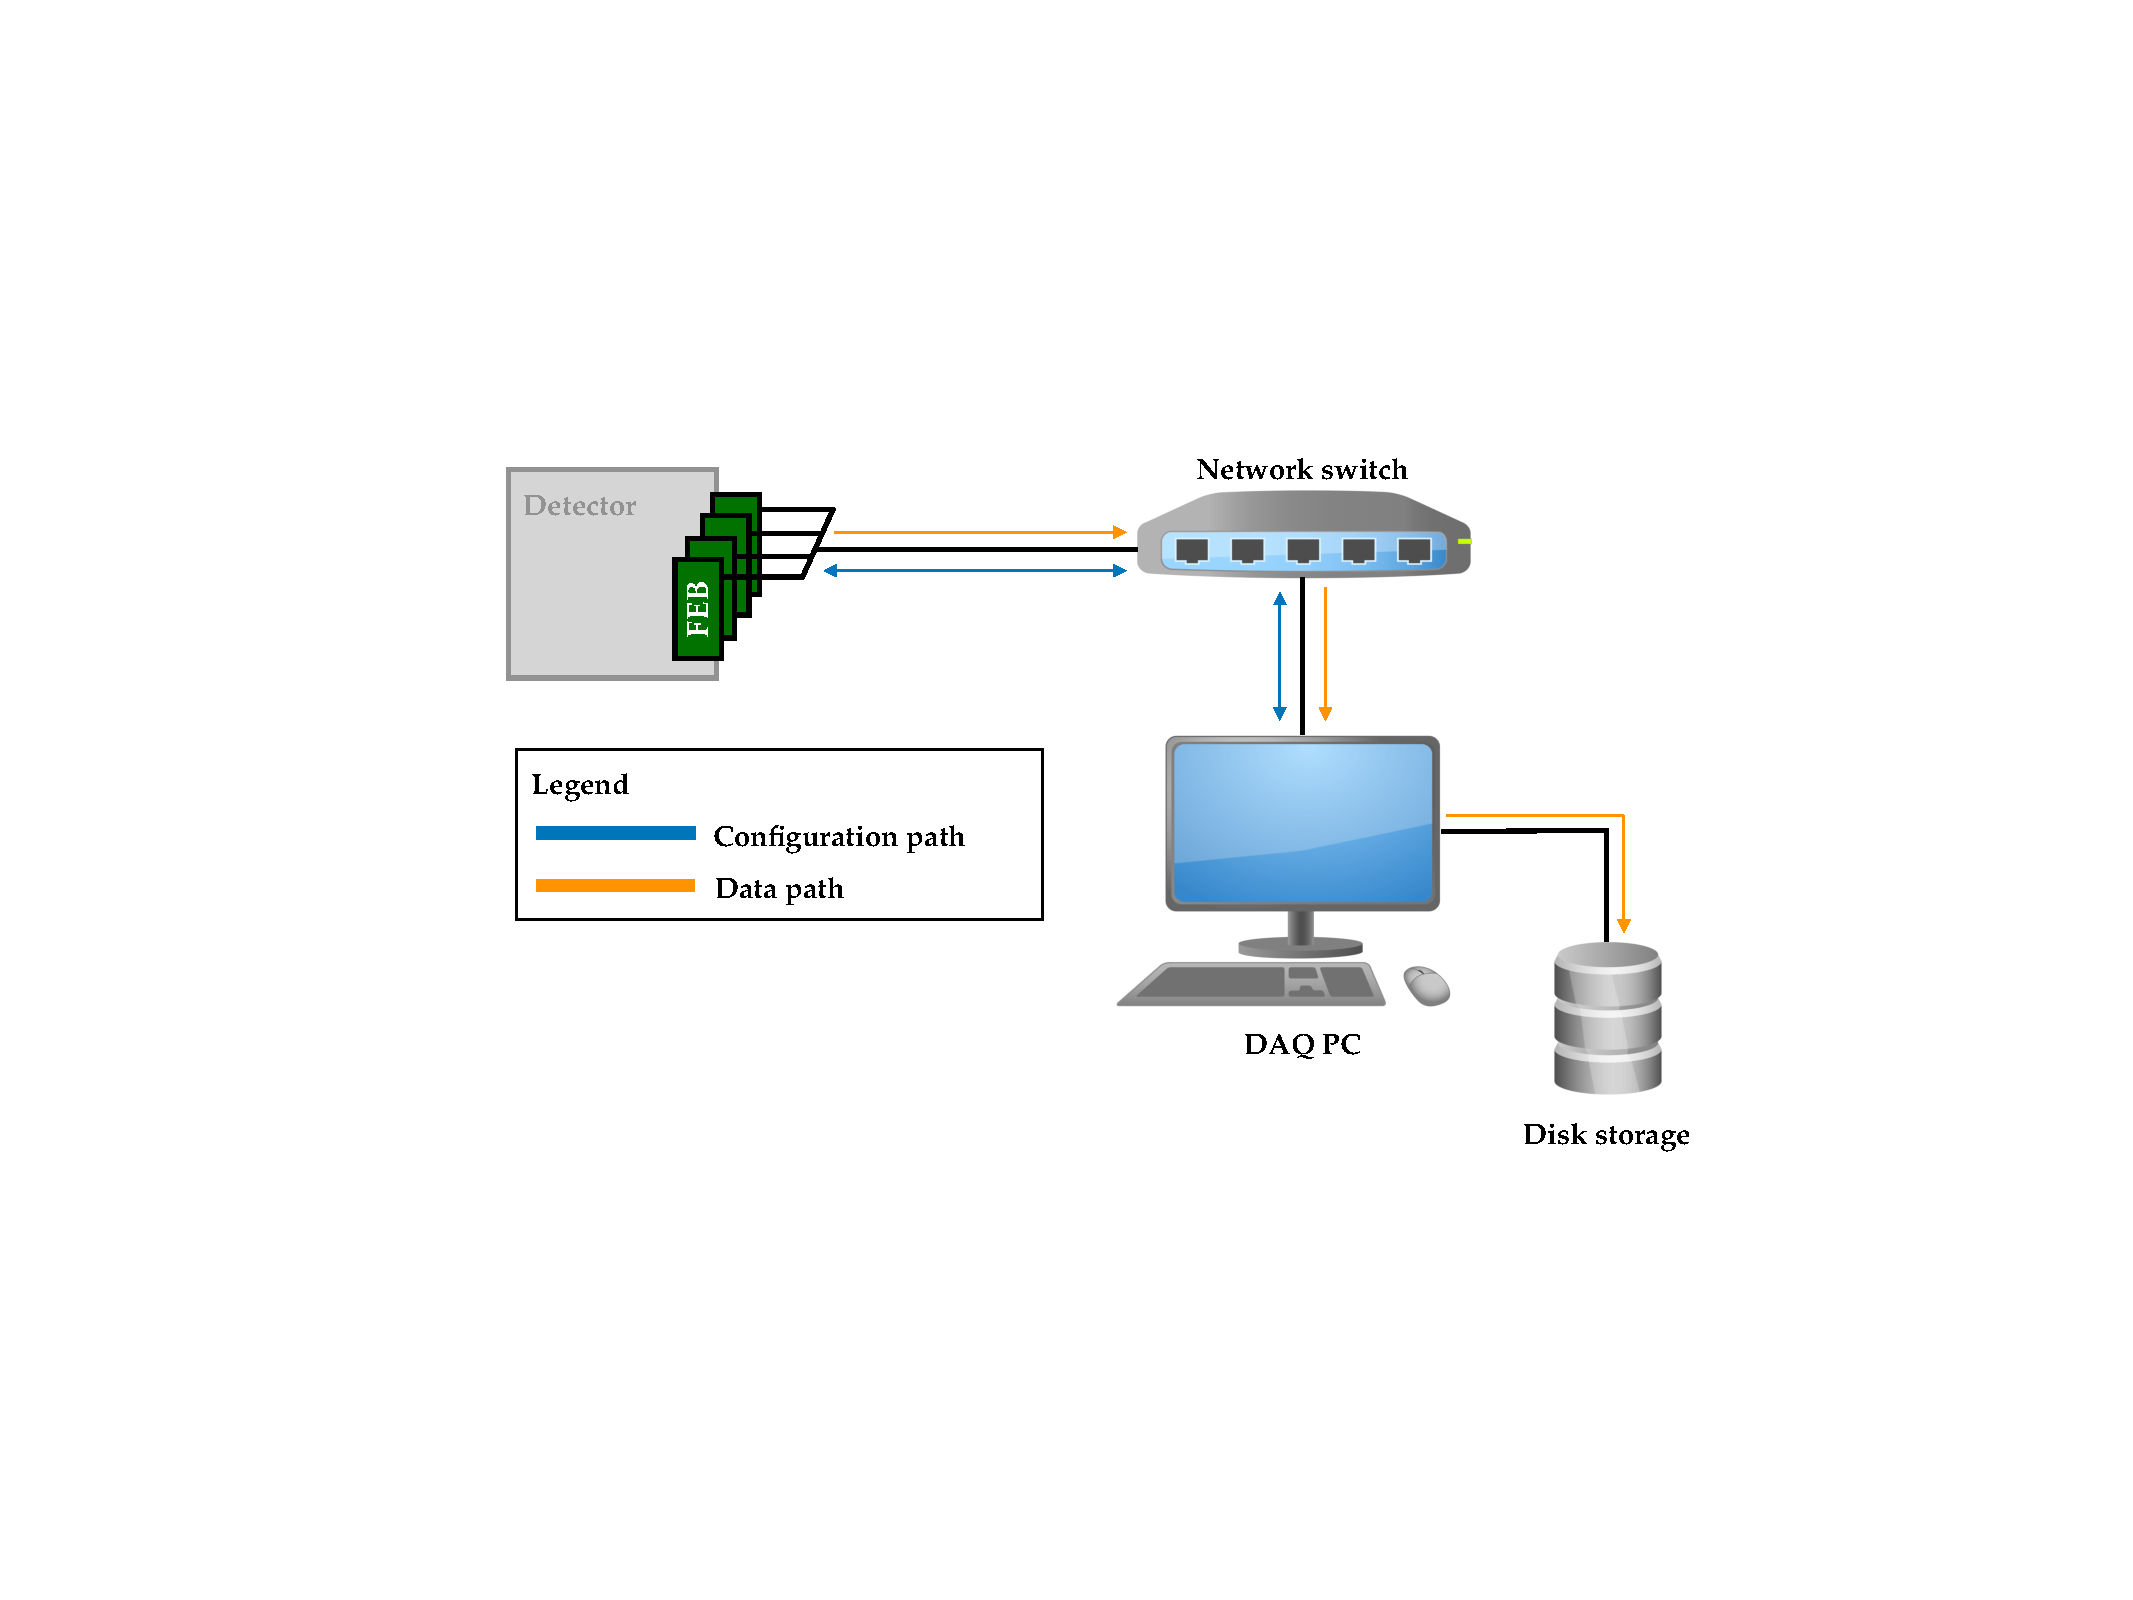
\includegraphics[width=0.5\textwidth]{figures/nsw/vrs/vrs_diagram_minimalPDF}
        \caption{
            A minimal VRS setup, in which a set of frontend boards (FEBs) are connected directly
            to the hosting DAQ PC.
            This setup is that typically used in labs and test benches, in which direct
            study of the VMM ASIC can be performed.
        }
        \label{fig:vrs_diagram_minimal}
    \end{center}
\end{figure}

\begin{figure}[!htb]
    \begin{center}
        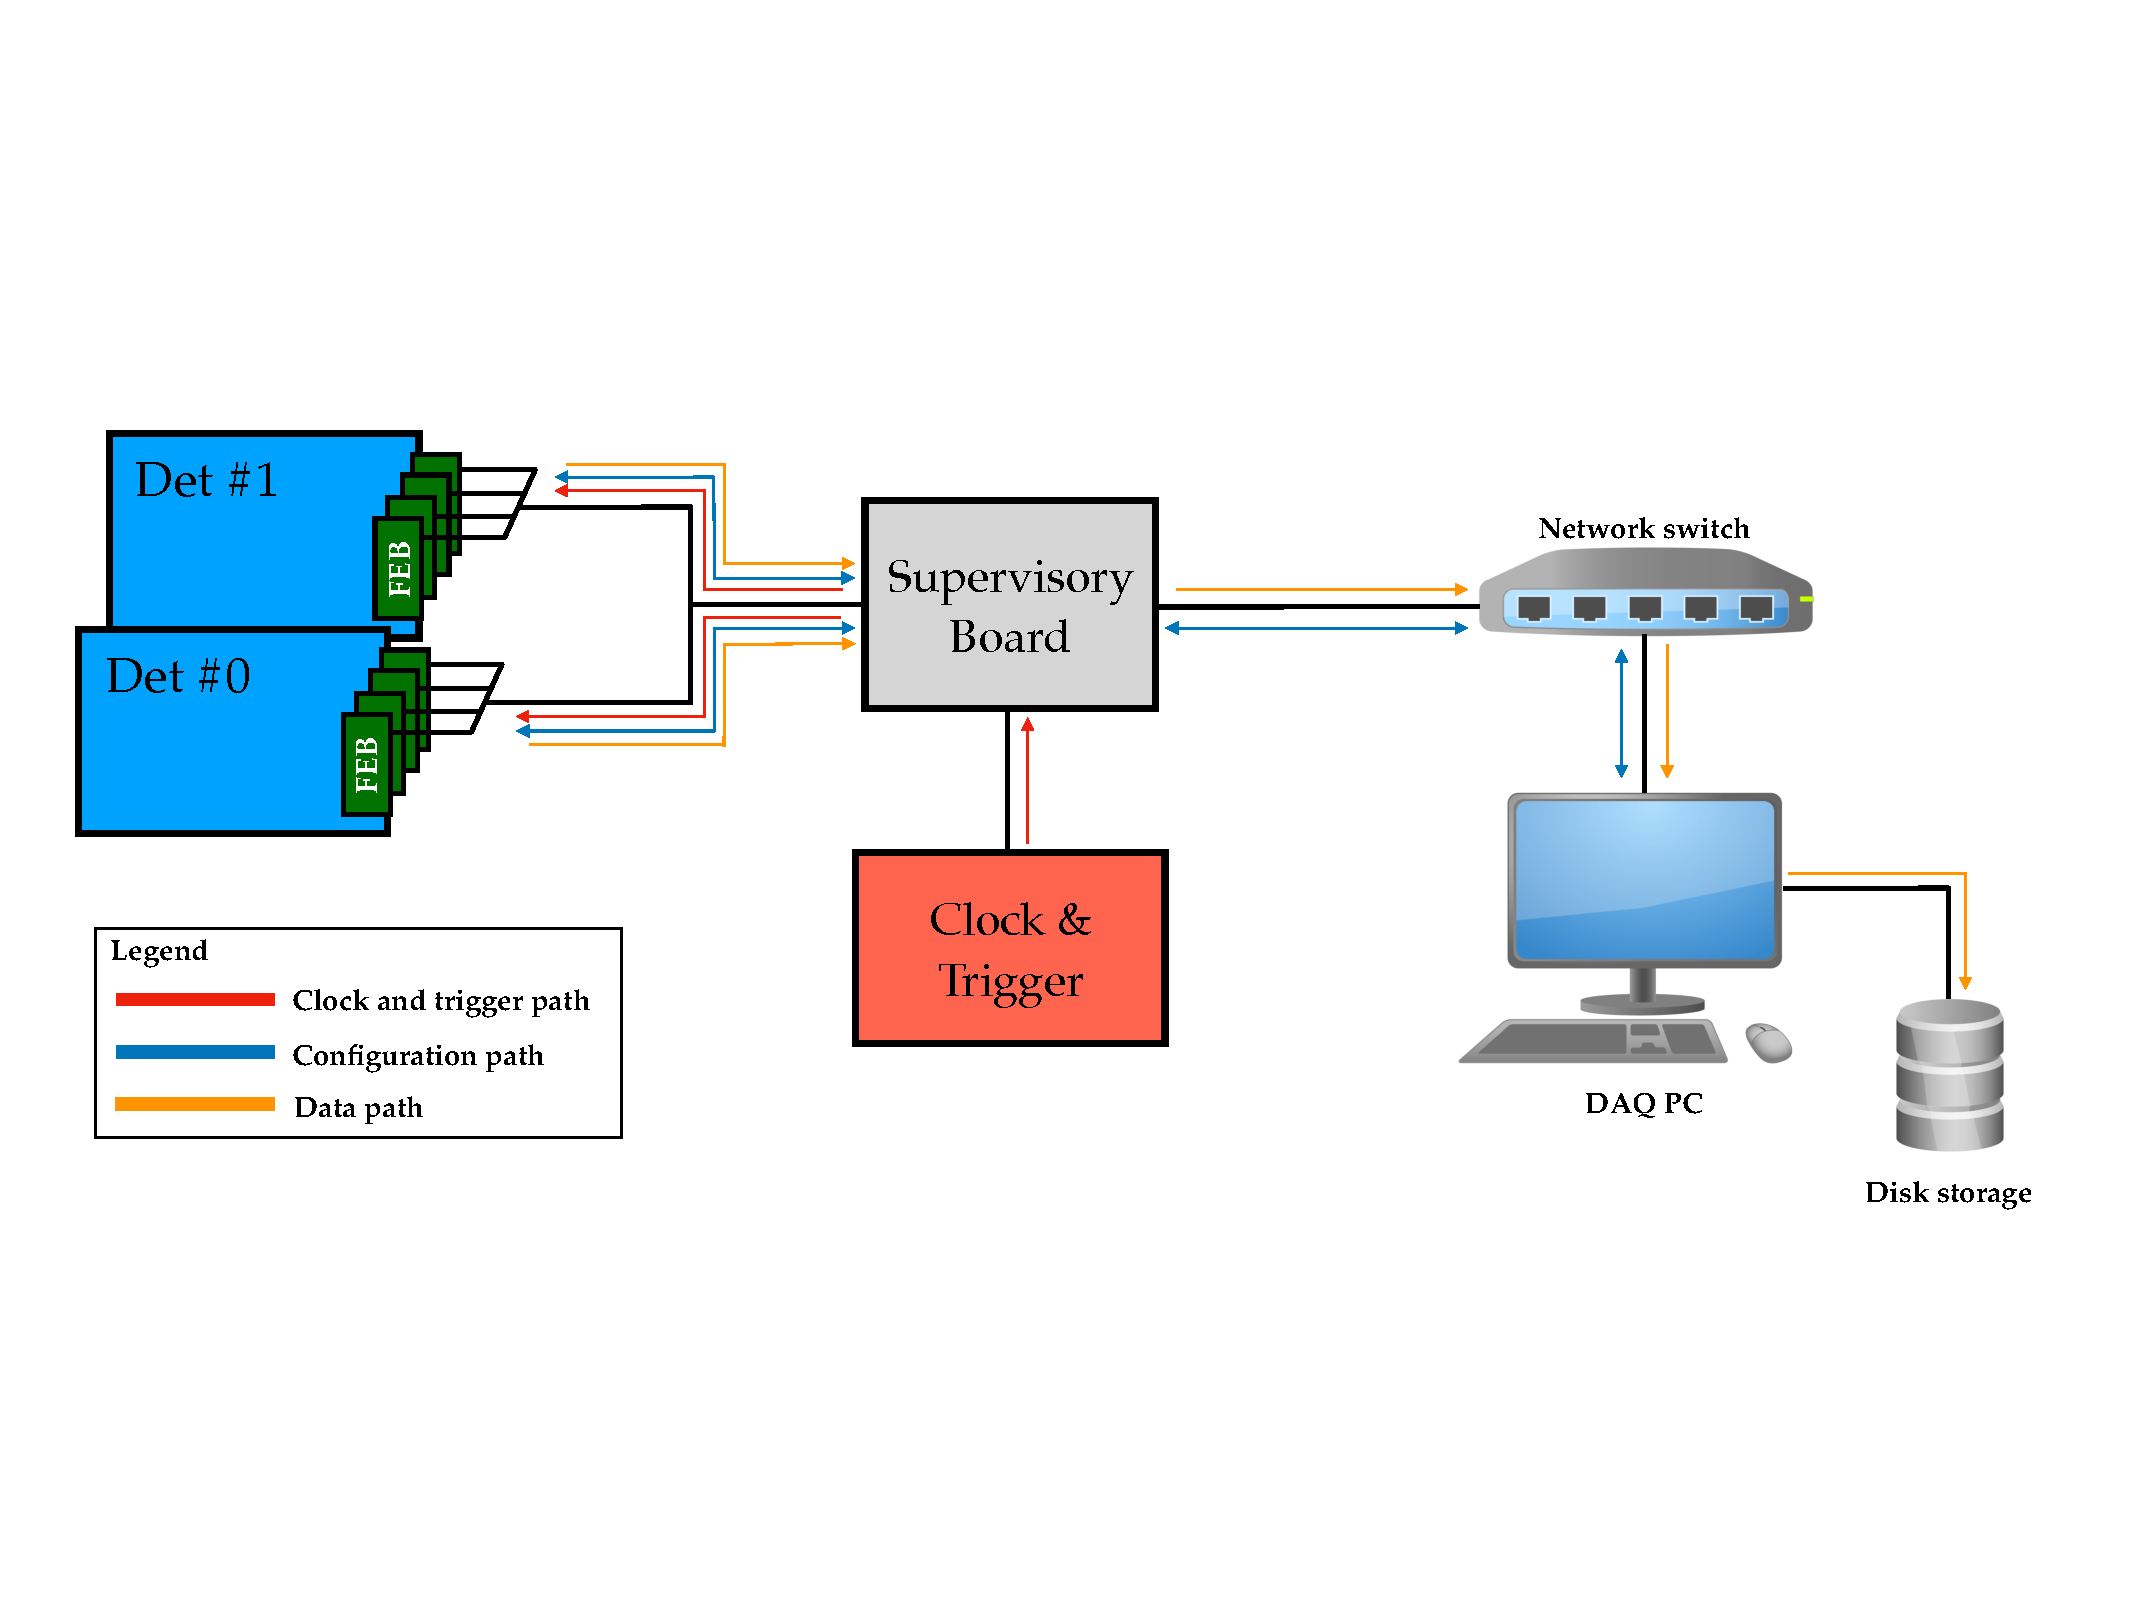
\includegraphics[width=0.7\textwidth]{figures/nsw/vrs/vrs_diagramPDF}
        \caption{
            A standard VRS setup, in which detector-grouped frontend boards (FEBs) receive external clock
            and trigger signals that are transmitted synchronously via the intermediate VRS Supervisory Board (VSB).
            This setup is used mainly for data taking scenarios in testbeams or in cosmic-ray stands.
        }
        \label{fig:vrs_diagram}
    \end{center}
\end{figure}
\FloatBarrier

%\subsection{VERSO}
%\label{sec:verso}

%\subsection{Calibration Algorithm Development}
%\label{sec:calib_alg}

%\subsubsection{Gain}
%\subsubsection{ADC Calibration}
%\subsubsection{Noise Measurements}
%\subsubsection{Timing Calibration}
%\subsubsection{Per-channel Threshold Equilisation}

\subsection{VERSO}
\label{sec:verso}

The software residing on the DAQ PC side (server side) of the VRS system,
illustrated in Figure~\ref{fig:vrs_diagram_minimal} and \ref{fig:vrs_diagram},
provides the main interface by which users can control the overall
state of the frontend electronics, either on- or off-detector,
as well as control the data acquisition and monitoring.
The high-level software suite containing these functionalities is referred
to as `VERSO', an acronym for `VMM Embedded ReadOut Software'.
In this section an overview of VERSO's role within the VRS system will be provided.

The user interface (UI) and software backend to VERSO are written entirely in the C++ programming langauge,
with the graphical user interface (GUI) relying primarily on the use of the Qt framework~\cite{QtCompany}.
The VERSO GUI is shown in Figure~\ref{fig:verso_main}.
VERSO has two main responsibilities: orchestrating configuration processes and
data-acquisition (DAQ).
Both functionalities are performed using a custom-made communication protocol
implemented in the UDP/IP communication protocol.
As illustrated in Figures~\ref{fig:vrs_diagram_minimal} and \ref{fig:vrs_diagram},
all communication from VERSO is sent over the network to either FPGAs located directly
on the frontend boards or on the VRS supervisory board, depending on the
data-taking situation.
The logical blocks indicated in Figure~\ref{fig:verso_main} are described as follows:

\begin{description}
    \item[] \textbf{Run Control} This block sets up the underlying configuration and DAQ
        that VERSO implements.
        From here the user can initiate and terminate the data taking sessions (`runs').
        VERSO supports several frontend types, either differing in the version of the VMM or in the
            implementation of the firmware (selected by the `VMM2', `VMM3', or `L0 R/O' buttons).
        The `Setup' and `Config' fields allow a user to load configuration files describing
            the detector-readout-element-to-VMM-channel mapping (detector geometry) and VMM ASIC configuration, respectively.\footnote{
                The detector-readout-element-to-VMM-channel mapping refers to both the geometric description
                of any detectors to which VERSO is communicating and the correspondence, for example, between an MM detector's
                strip location to the frontend board and VMM channel responsible for reading out that MM strip's signals.
                This correspondence is required if one wishes to construct high level objects, such as
                particle tracks, traversing through several detector layers and with each layer read out
                by different frontend boards.
            }
    \item[] \textbf{Network Communication} This block describes the network addresses of the
        frontend electronics and handles the sustained connection to them.
    \item[] \textbf{FPGA and Operational Parameters} This block sets the configuration parameters
            for the FPGA on the connected frontend boards. Such parameters, for example,
            are the frequency and width of the VMM channel test pulse signal and the bunch
            crossing clock driving the readout of the VMM ASIC.
    \item[] \textbf{Message Reporting} Reports messages visually so that the user may acknowledge
            the current state of the system. Sends messages also to files stored on the DAQ PC.
    \item[] \textbf{VMM Configuration Panel} The `Global Registers' and `Channel Registers' panels allow
        the user to set the configuration parameters of the VMM ASICs on the frontend boards.
        An instance of the VMM Channel Registers panel is shown in Figure~\ref{fig:verso_chanreg}.
    \item[] \textbf{VMM Calibration Panel} This panel allows the user to schedule various VMM calibration routines.
        The user may also provide files containing calibration constants/parameters, derived from previous
        calibration runs, that get loaded into the associated VMM configuration
        bitstreams during subsequent VMM configuration processes.
\end{description}

\noindent The configuration of the FPGA is sent over the network from VERSO and
follows an address-value mechanism whereby each configurable parameter of the FPGA has its
value stored within the FPGA at a specific memory register.
VERSO sets an FPGA configurable parameter by forwarding a register address followed by its corresponding
value as specified by the user.
The FPGA sends acknowledgement packets over the network to VERSO upon each message received,
indicating whether it was able to successfully perform the requested configuration action or not.
If not, VERSO can log this information and re-attempt transmission of the lost or mis-handled packet
containing the configuration specification.
%The configuration of the VMM ASICs is forwarded by the FPGA via the Serial Peripheral Interface (SPI) protocal
%to the VMMs.
The VMM ASIC recieves its own configuration following a Serial Peripheral Interface (SPI) protocol.\footnote{\url{https://en.wikipedia.org/wiki/Serial_Peripheral_Interface}}
An individual VMM ASIC configuration specification is rather large and is nearly 2 kilobits long.
This large configuration bitstream is due to the highly configurable nature of the VMM ASIC, especially
so given that each of the 64 channels of a single VMM has 24 bits worth of configuration information.
%An individual VMM ASIC configuration is rather large, given its highly configurable nature, and is
%nearly 2 kilobits long.
The specification of the VMM configuration bitstreams is set by the user in the `Global' and `Channel' configuration
panels on the GUI, shown in Figure~\ref{fig:verso_main}.
The `Global' VMM parameters are those that are not specific to an individual channel; for example,
the VMM channel threshold, channel gain, or the specification of the VMM signal shaper's integration time.
The VERSO software handles the construction of the configuration bitstreams for each VMM ASIC and forwards
them to the corresponding FPGA that is directly connected to the VMM to be configured.
Upon receipt of a VMM configuration bitstream, the FPGA forwards it to the SPI input of the specified VMM.
The FPGA knows to which of the (potentially several) on-board VMMs to forward the configuration based on
a custom addressing dataframe parsed by the FPGA that VERSO prepends to each configuration bitstream.

\begin{figure}[!htb]
    \begin{center}
        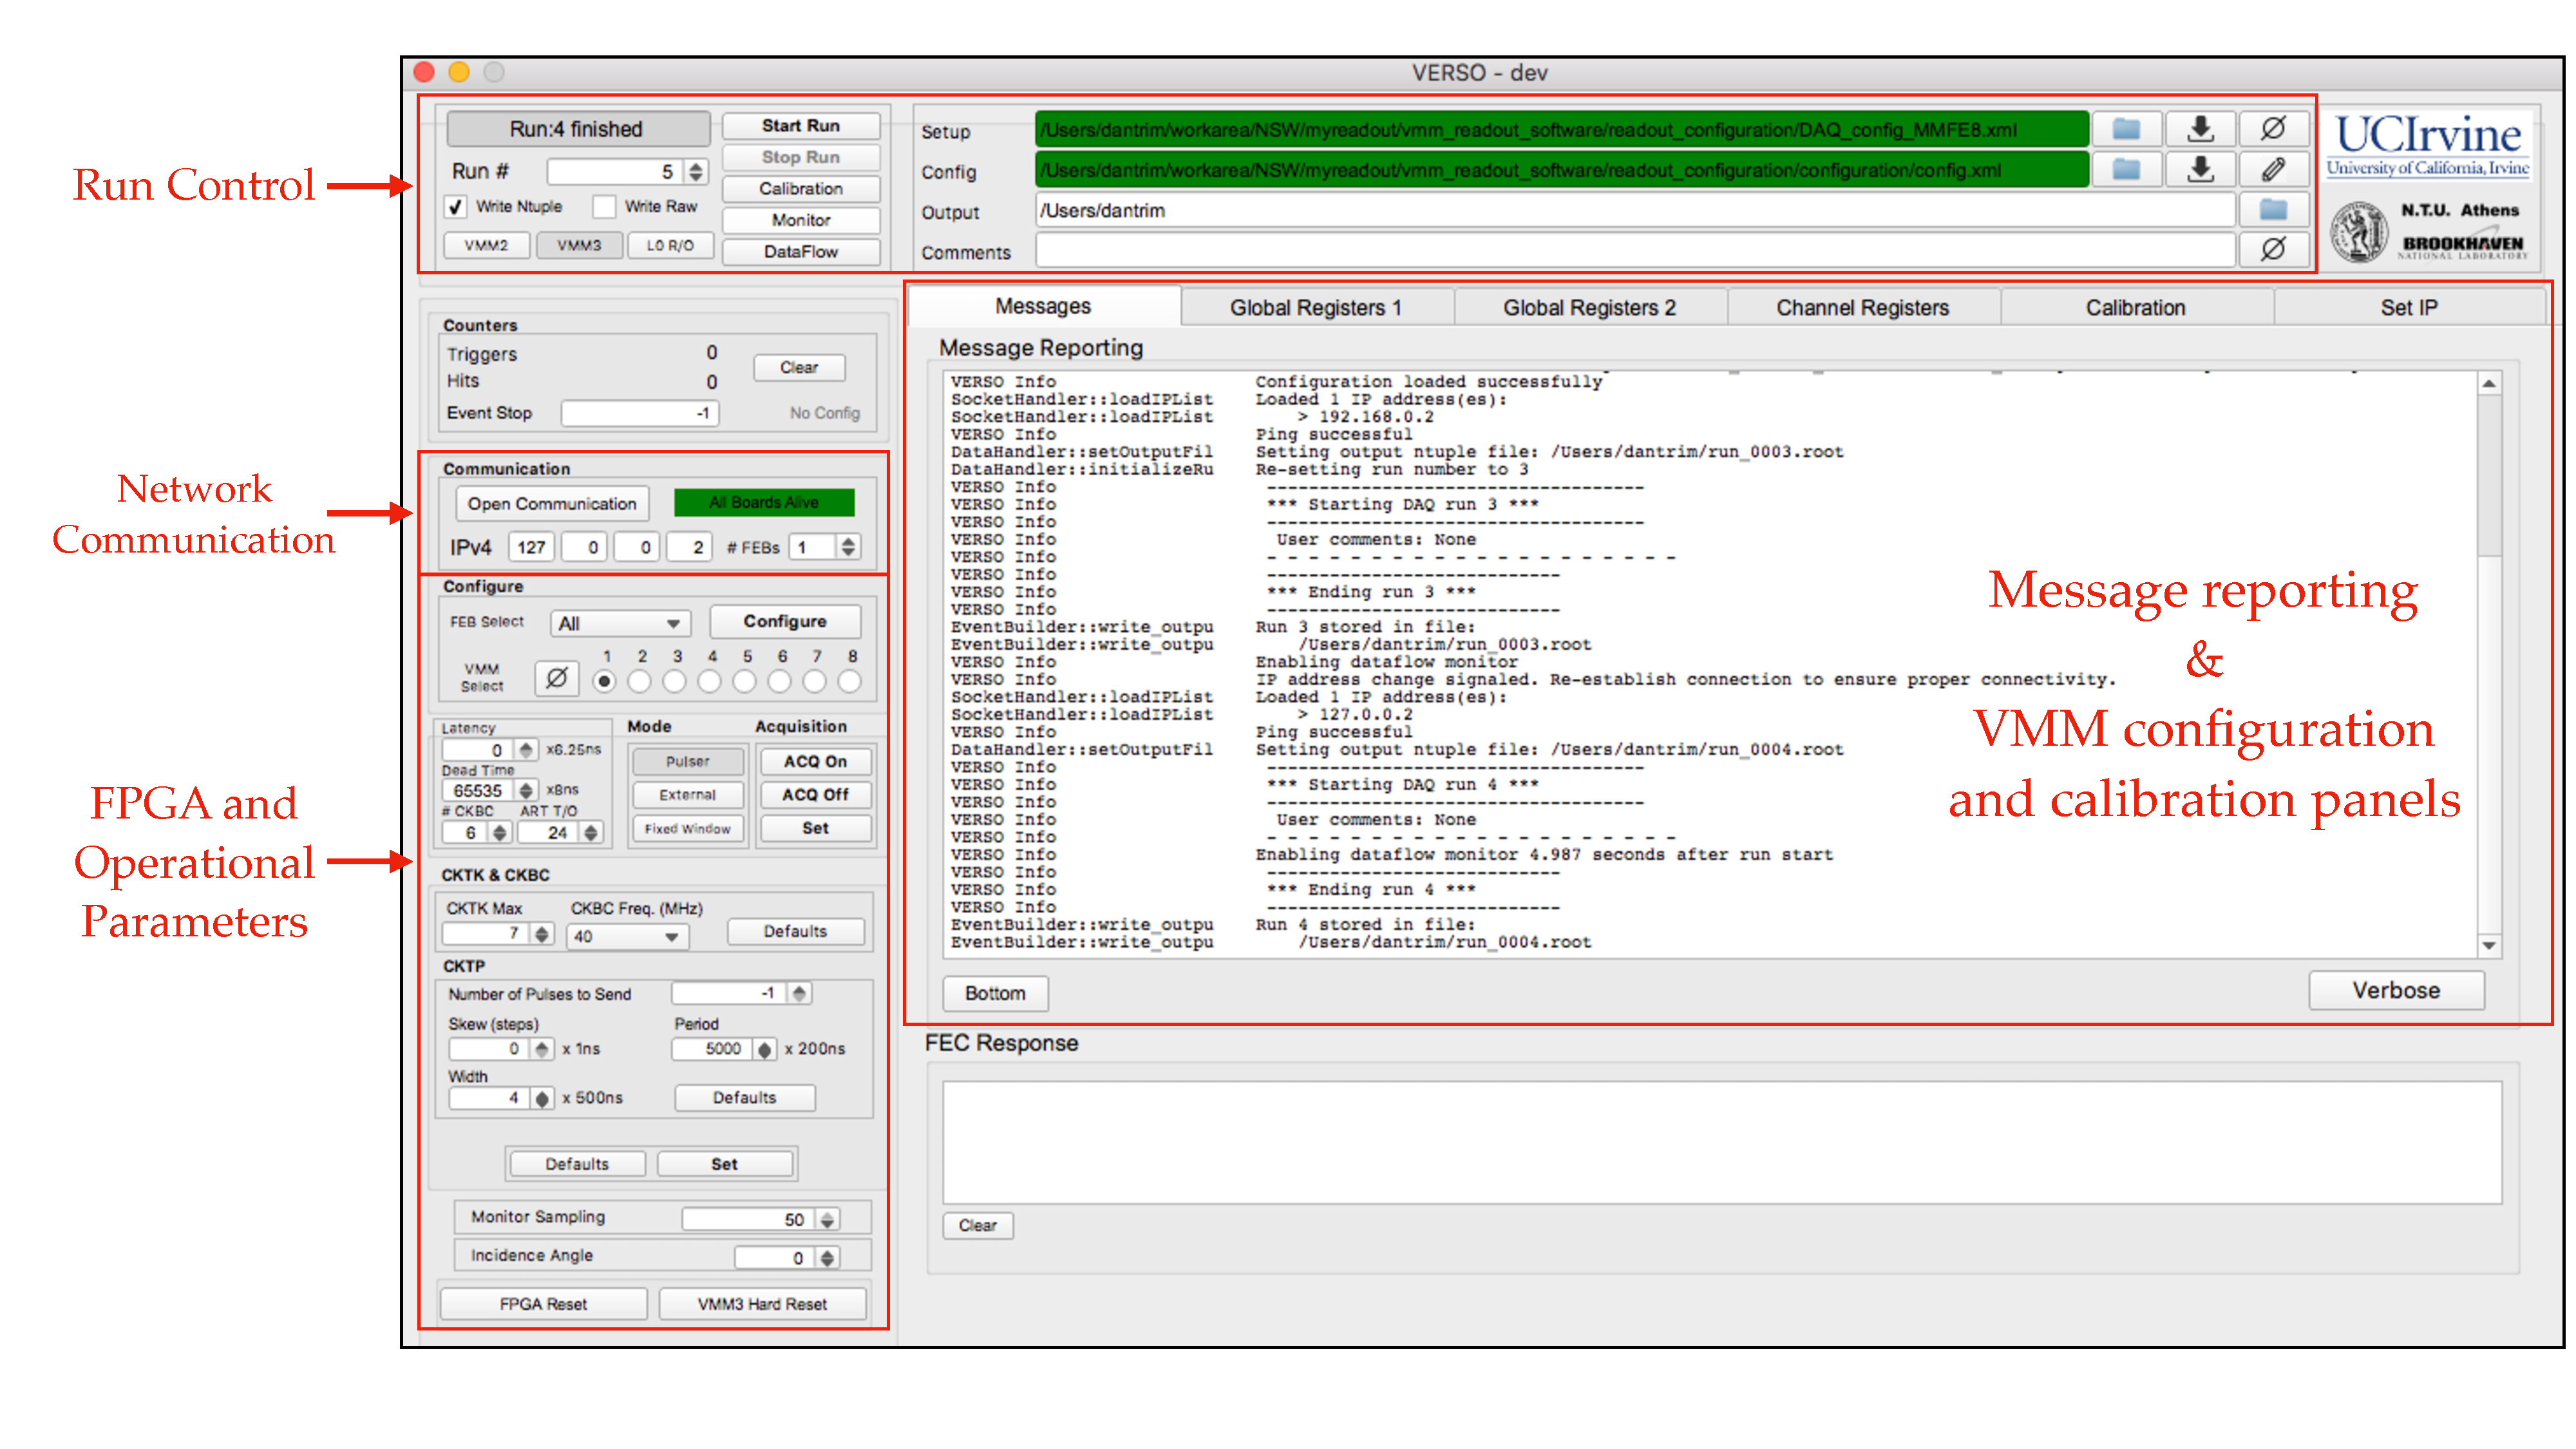
\includegraphics[width=0.95\textwidth]{figures/nsw/vrs/verso_mainPDF}
        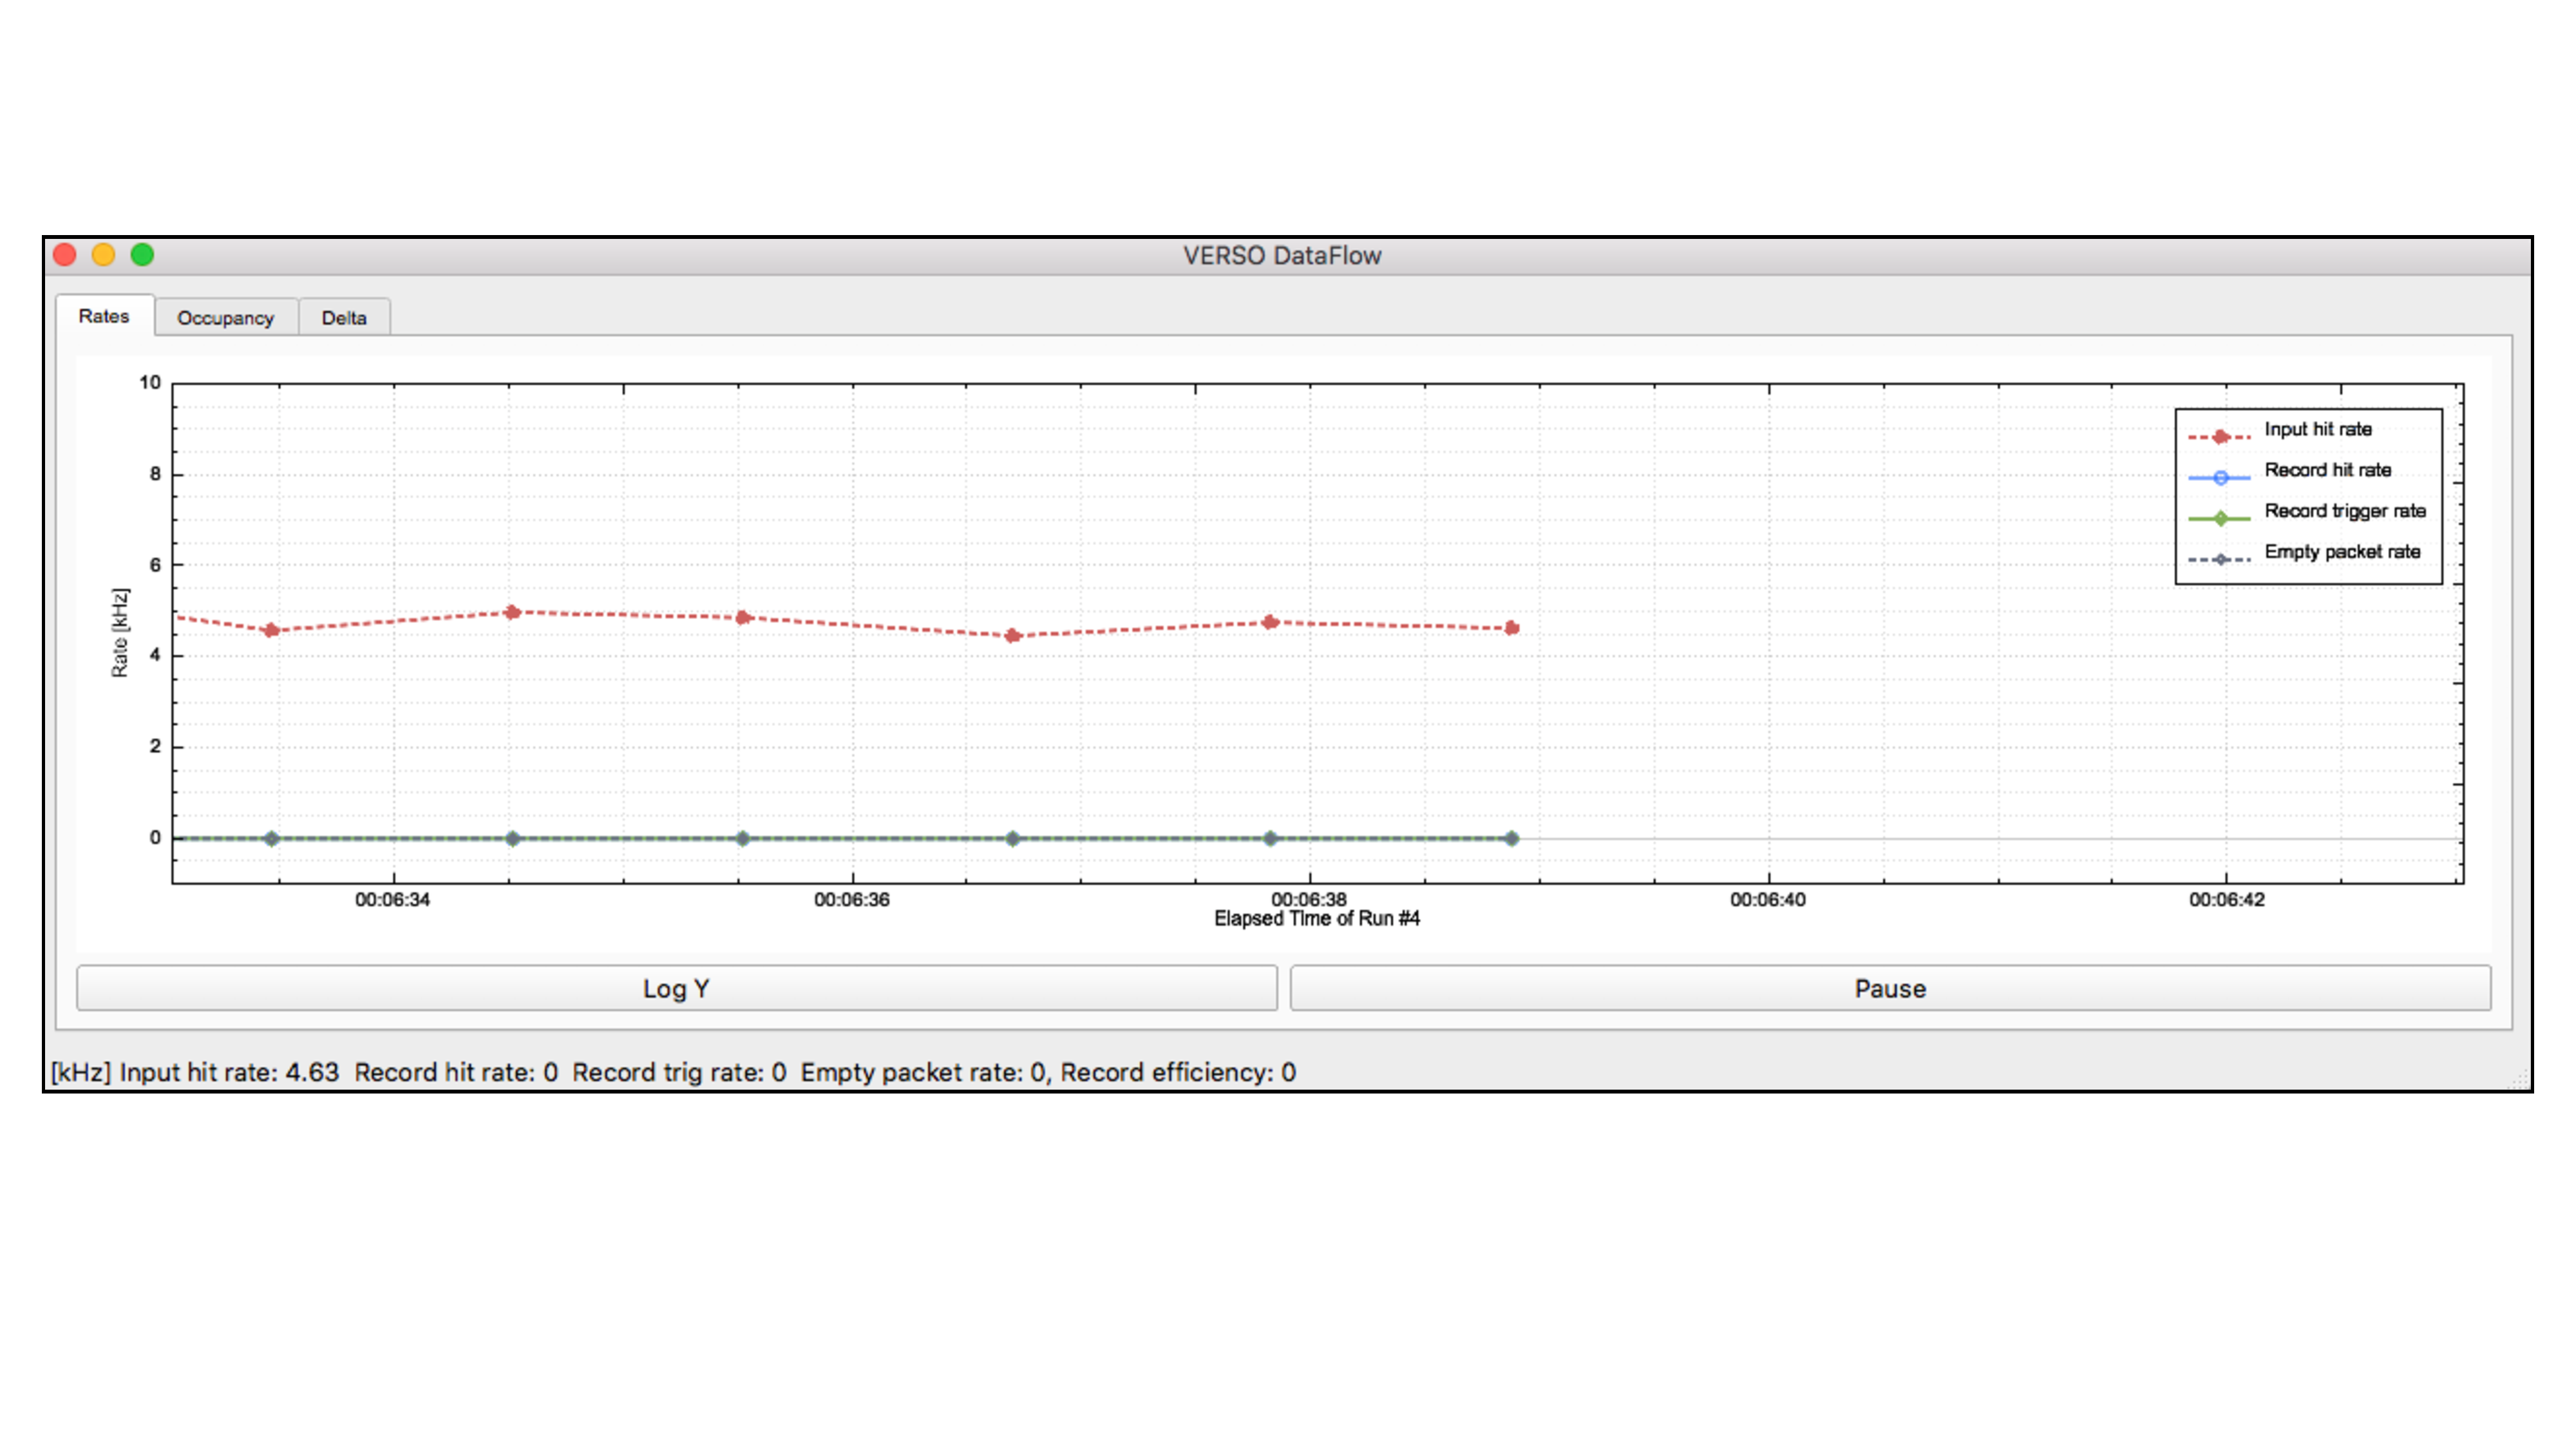
\includegraphics[width=0.8\textwidth]{figures/nsw/vrs/verso_dataflow}
        \caption{
            \textbf{\textit{Top}}: Main VERSO user interface, with different logical blocks indicated.
            \textbf{\textit{Bottom}}: VERSO dataflow monitor, showing the rate of VMM channel hits
                for all connected frontend boards and VMMs. Also displayed are the rate at which individual
                hits and events are recorded, where an `event' is a collection of hits associated with the
                same trigger.
                The data being shown in this graph correspond to hits generated with the VMM channel
                test pulse injection with the output data recording disabled.
                The DAQ efficiency, defined in Equation~\ref{eq:verso_daq_eff}, can be observed on this graph
                by dividing the blue line by the red line.
        }
        \label{fig:verso_main}
    \end{center}
\end{figure}

\begin{figure}[!htb]
    \begin{center}
        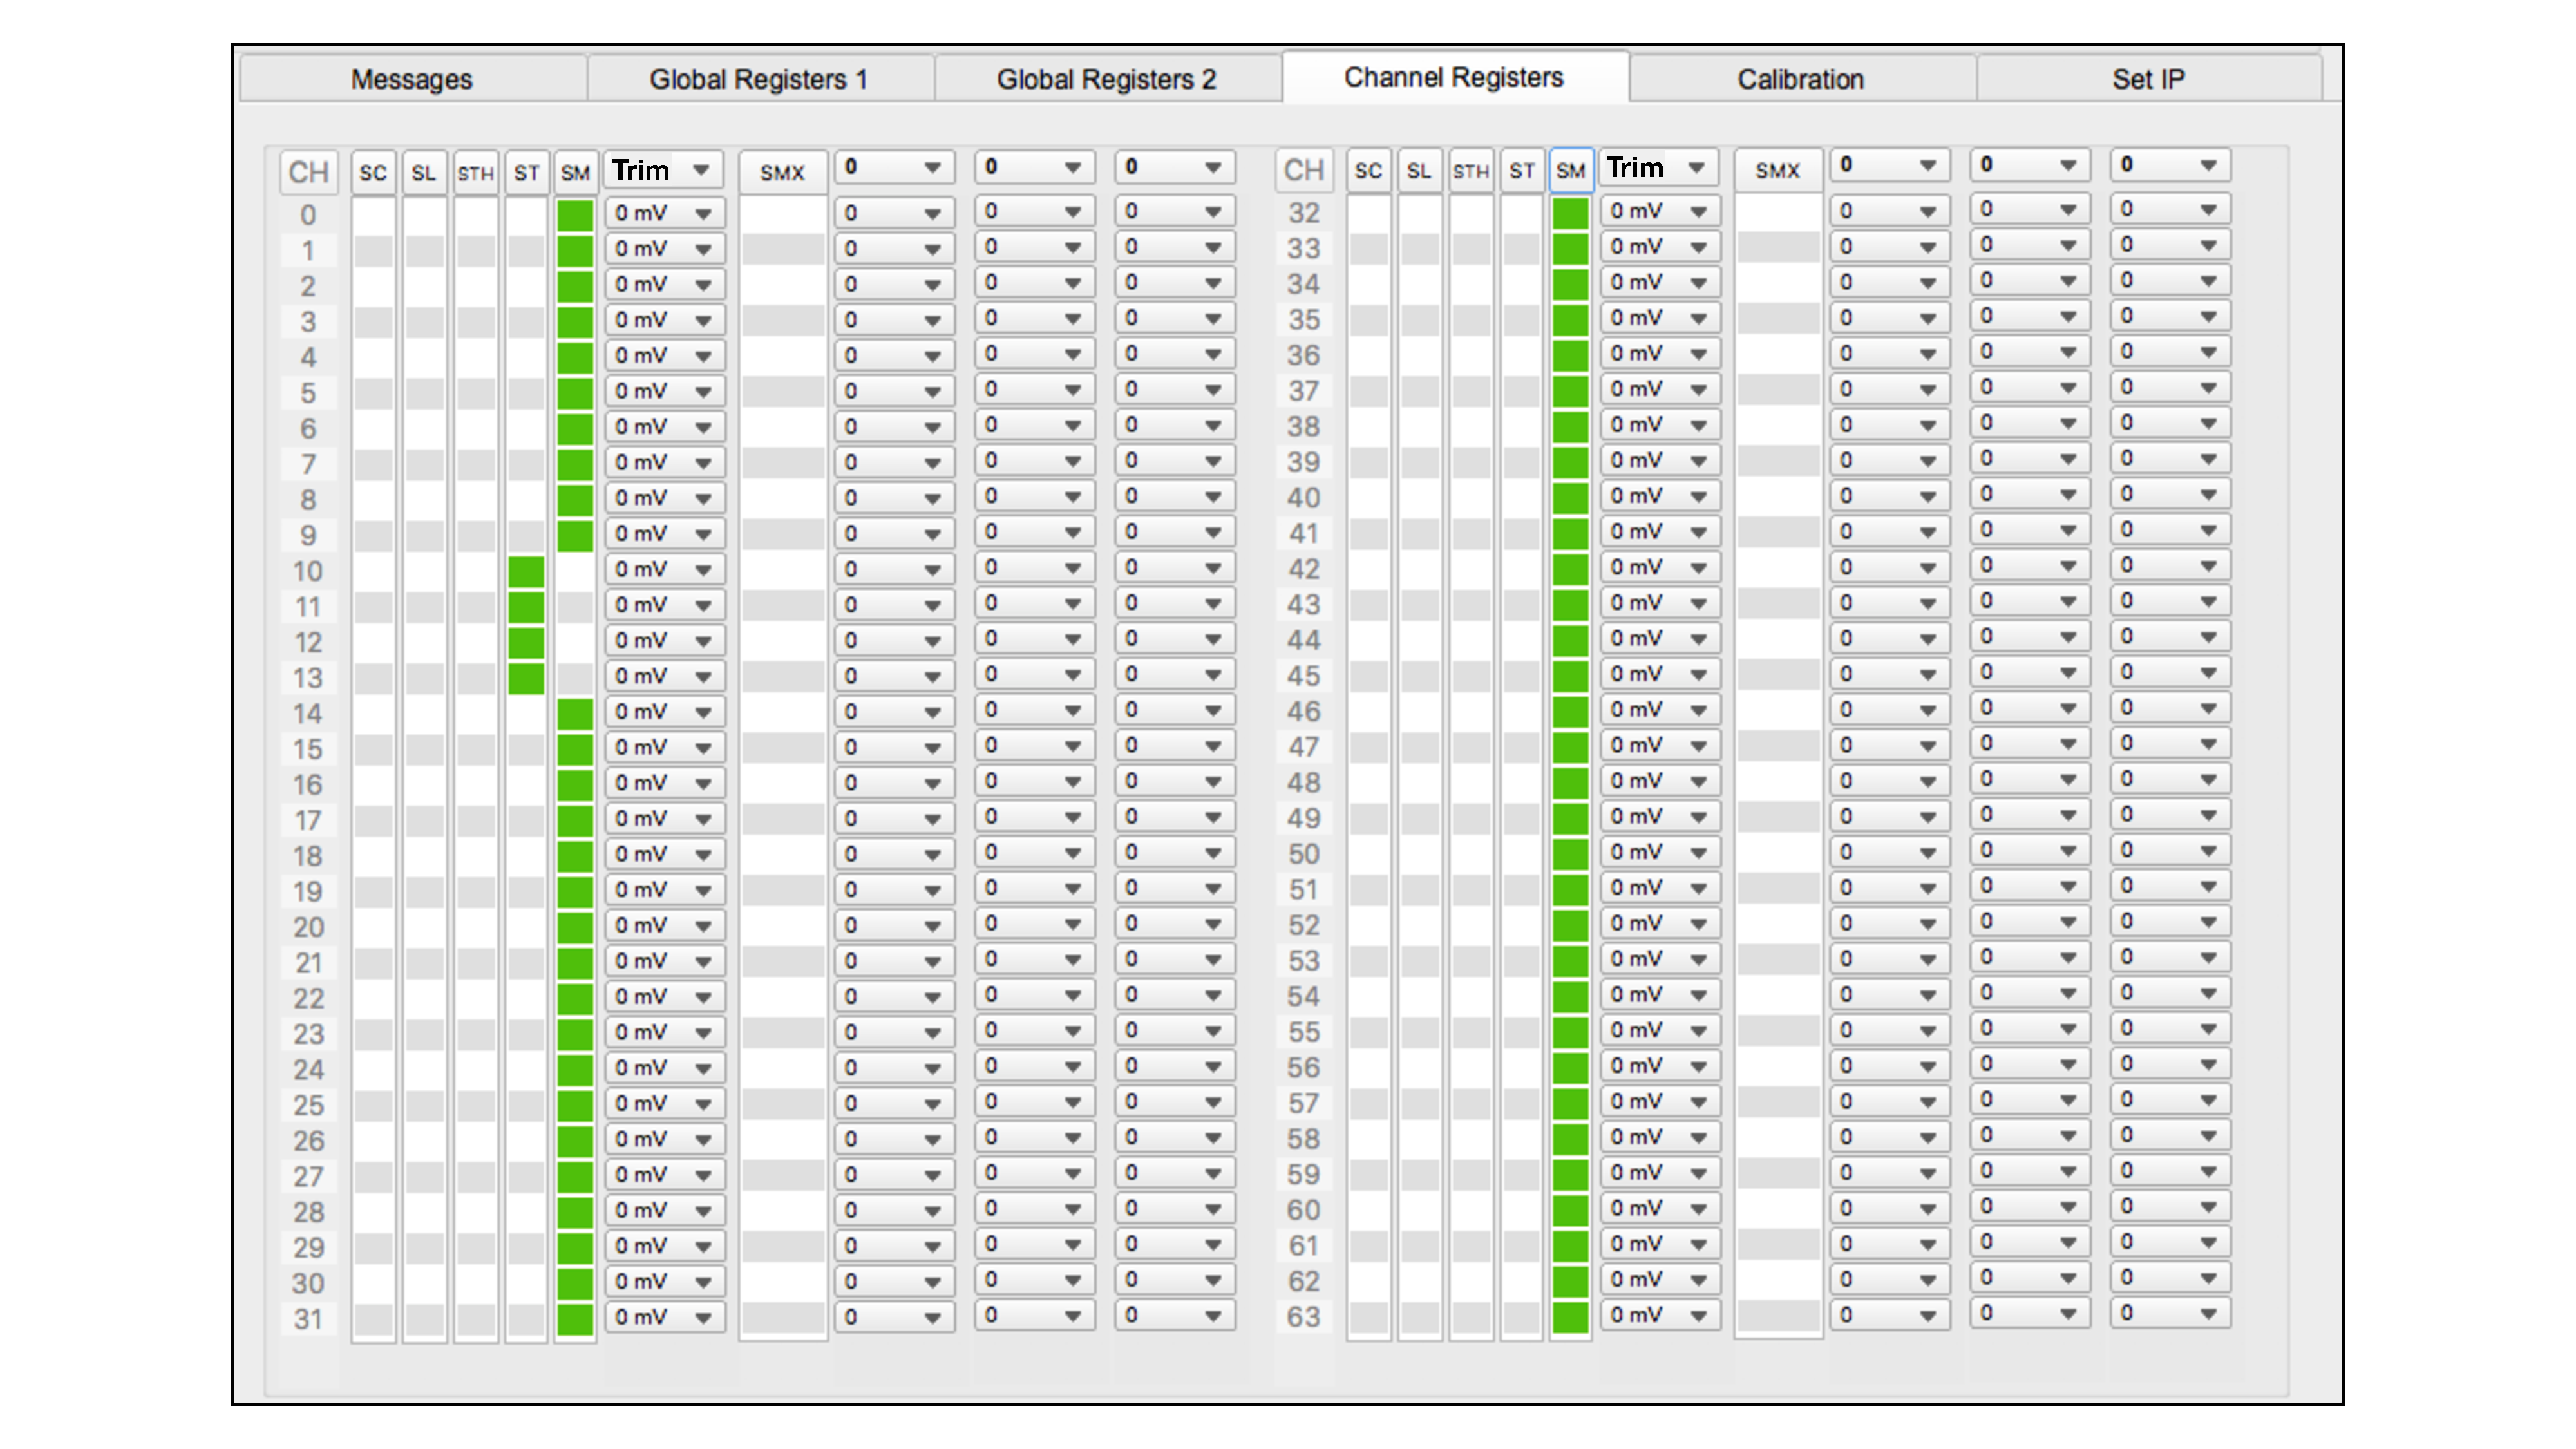
\includegraphics[width=0.8\textwidth]{figures/nsw/vrs/verso_chanreg}
        \caption{
            The VERSO `Channel Registers' panel, showing the configuration specification
            of each of the 64 channels of an individual VMM.
            The `ST' (`SM') flags activate the corresonding channel's internal test-charge
            capacitor (masking).
            In the example shown, VMM channels 10-13 (inclusive) will have their
            test-charge capacitor activated. All other channels are masked and
            are effectively disabled.
            The `Trim' configuration refers to the 5-bit channel threshold trimming,
            specifying by how much the individual channel's threshold should be moved
            relative to the global VMM threshold value.
        }
        \label{fig:verso_chanreg}
    \end{center}
\end{figure}

The VERSO DAQ backend is responsible for handing the readout of the frontend boards.
VMM hit data is sent over the network and received by VERSO.
The hit data may be that of a detector being readout by the VMM-based frontend electronics
or simulated data created by the individual VMM channel test-charge capacitors that can inject
signal onto each of the VMM channel inputs.
In the latter case, the frequency and characteristics (width, amplitude, etc...) of the
signals are specified via the FPGA configuration described above, since the FPGA orchestrates
the triggering of the VMM channel test-charge injection signals.

VERSO's DAQ functionalities are implemented following a single-producer/single-consumer
architecture.
In such an architecture, at the start of each run, the software constructs two threads with independent
tasks: a `listener' thread and an `event builder' thread.
The listener thread is reponsible for receiving the raw digitised data packets over the network from the
frontend electronics and buffering them in a queue.
The listener thread indexes each of the data fragments in the queue based on their corresponding
event or trigger identifier.
VMM hit data corresponding to the same trigger will all be given the
same such identifier.
For each received trigger identifier, the event builder thread collects the associated data fragments from
the queue so that all fragments from a given event may be handled at a single time.
The event builder thread is responsible for decoding and inspecting the raw data contained in these fragments and building
an output data structure that represents high-level constructs related to the event as a whole: associating
the event's VMM hits with specific frontend boards and/or detector readout elements, for example.
It is this latter aspect --- the gathering together of all data fragments corresponding to a specific trigger ---
that is referred to as `event building'.
Once such an event is built, VERSO stores it on disk in the ROOT \texttt{TTree} format
so that it may be used in later offline analysis.
%The event builder thread is responsible for taking all the data fragments from a given trigger identifier,
%The second thread is responsible for taking all the data fragments received for each corresponding
%trigger, decoding and inspecting the raw data contained therein, and building output
%data fragments that represent high level constructs that associate the VMM hits
%with specicific frontend boards and/or detector readout elements.
%This latter aspect --- the gathering together of all data fragments corresponding to a
%specific trigger --- is referred to as `event building'.
%Once an event is built, VERSO stores it on disk in the ROOT \texttt{TTree} format
%for later analysis.

Given the asynchronous nature of the network communication, as well as the fact that the UDP/IP
network protocol does not ensure a fixed latency, events based on the same trigger
are not guaranteed to be captured by VERSO within the same UDP/IP network packet if there are multiple frontend boards being read out.
The use of the single-producer/single-consumer model is adapted to such a case, with
the producer (listener) thread indexing and filling the queue and the consumer thread performing the event building.
In VERSO, the queue in which indexed data fragments are stored is implemented
as a lock-free\footnote{\url{https://en.wikipedia.org/wiki/Non-blocking_algorithm}} concurrent queue.
As a result, the queue may be accessed and manipulated by each thread without affecting or blocking
the other, allowing for smooth DAQ operation.
The event building thread can then periodically inspect the queue and wait for a configurable amount of time for the expected
number of data fragments from each of the frontend elements before finishing
the event building process.
Once the event building process is completed,
the event building thread starts the process over and begins gathering the data fragments from the next-received trigger number identifier.
The use of the multi-threaded architecture, pivoting around a fast concurrent queue
implementation,\footnote{\url{http://moodycamel.com/blog/2013/a-fast-lock-free-queue-for-c++}}
has allowed VERSO to achieve 100\% DAQ efficiency
in all use-cases encountered ({\color{red}{Section XXX for use-cases}}).
Here the DAQ efficiency is defined as,
\begin{align}
    \varepsilon_{\text{DAQ}} = \frac{ N_{\text{recorded}} }{ N_{\text{expected}} },
    \label{eq:verso_daq_eff}
\end{align}
where $N_{\text{recorded}}$ is the number of events stored on disk by the event building
thread and $N_{\text{expected}}$ is the total number of event data fragments sent
over the network to VERSO from the frontend electronics.
The latter number, $N_{\text{expected}}$, can be determined via counters located
on the FPGAs on the frontend.

\FloatBarrier

\subsection{Calibration of the VMM ASIC}
\label{sec:calib_alg}

\begin{figure}[!htb]
    \begin{center}
        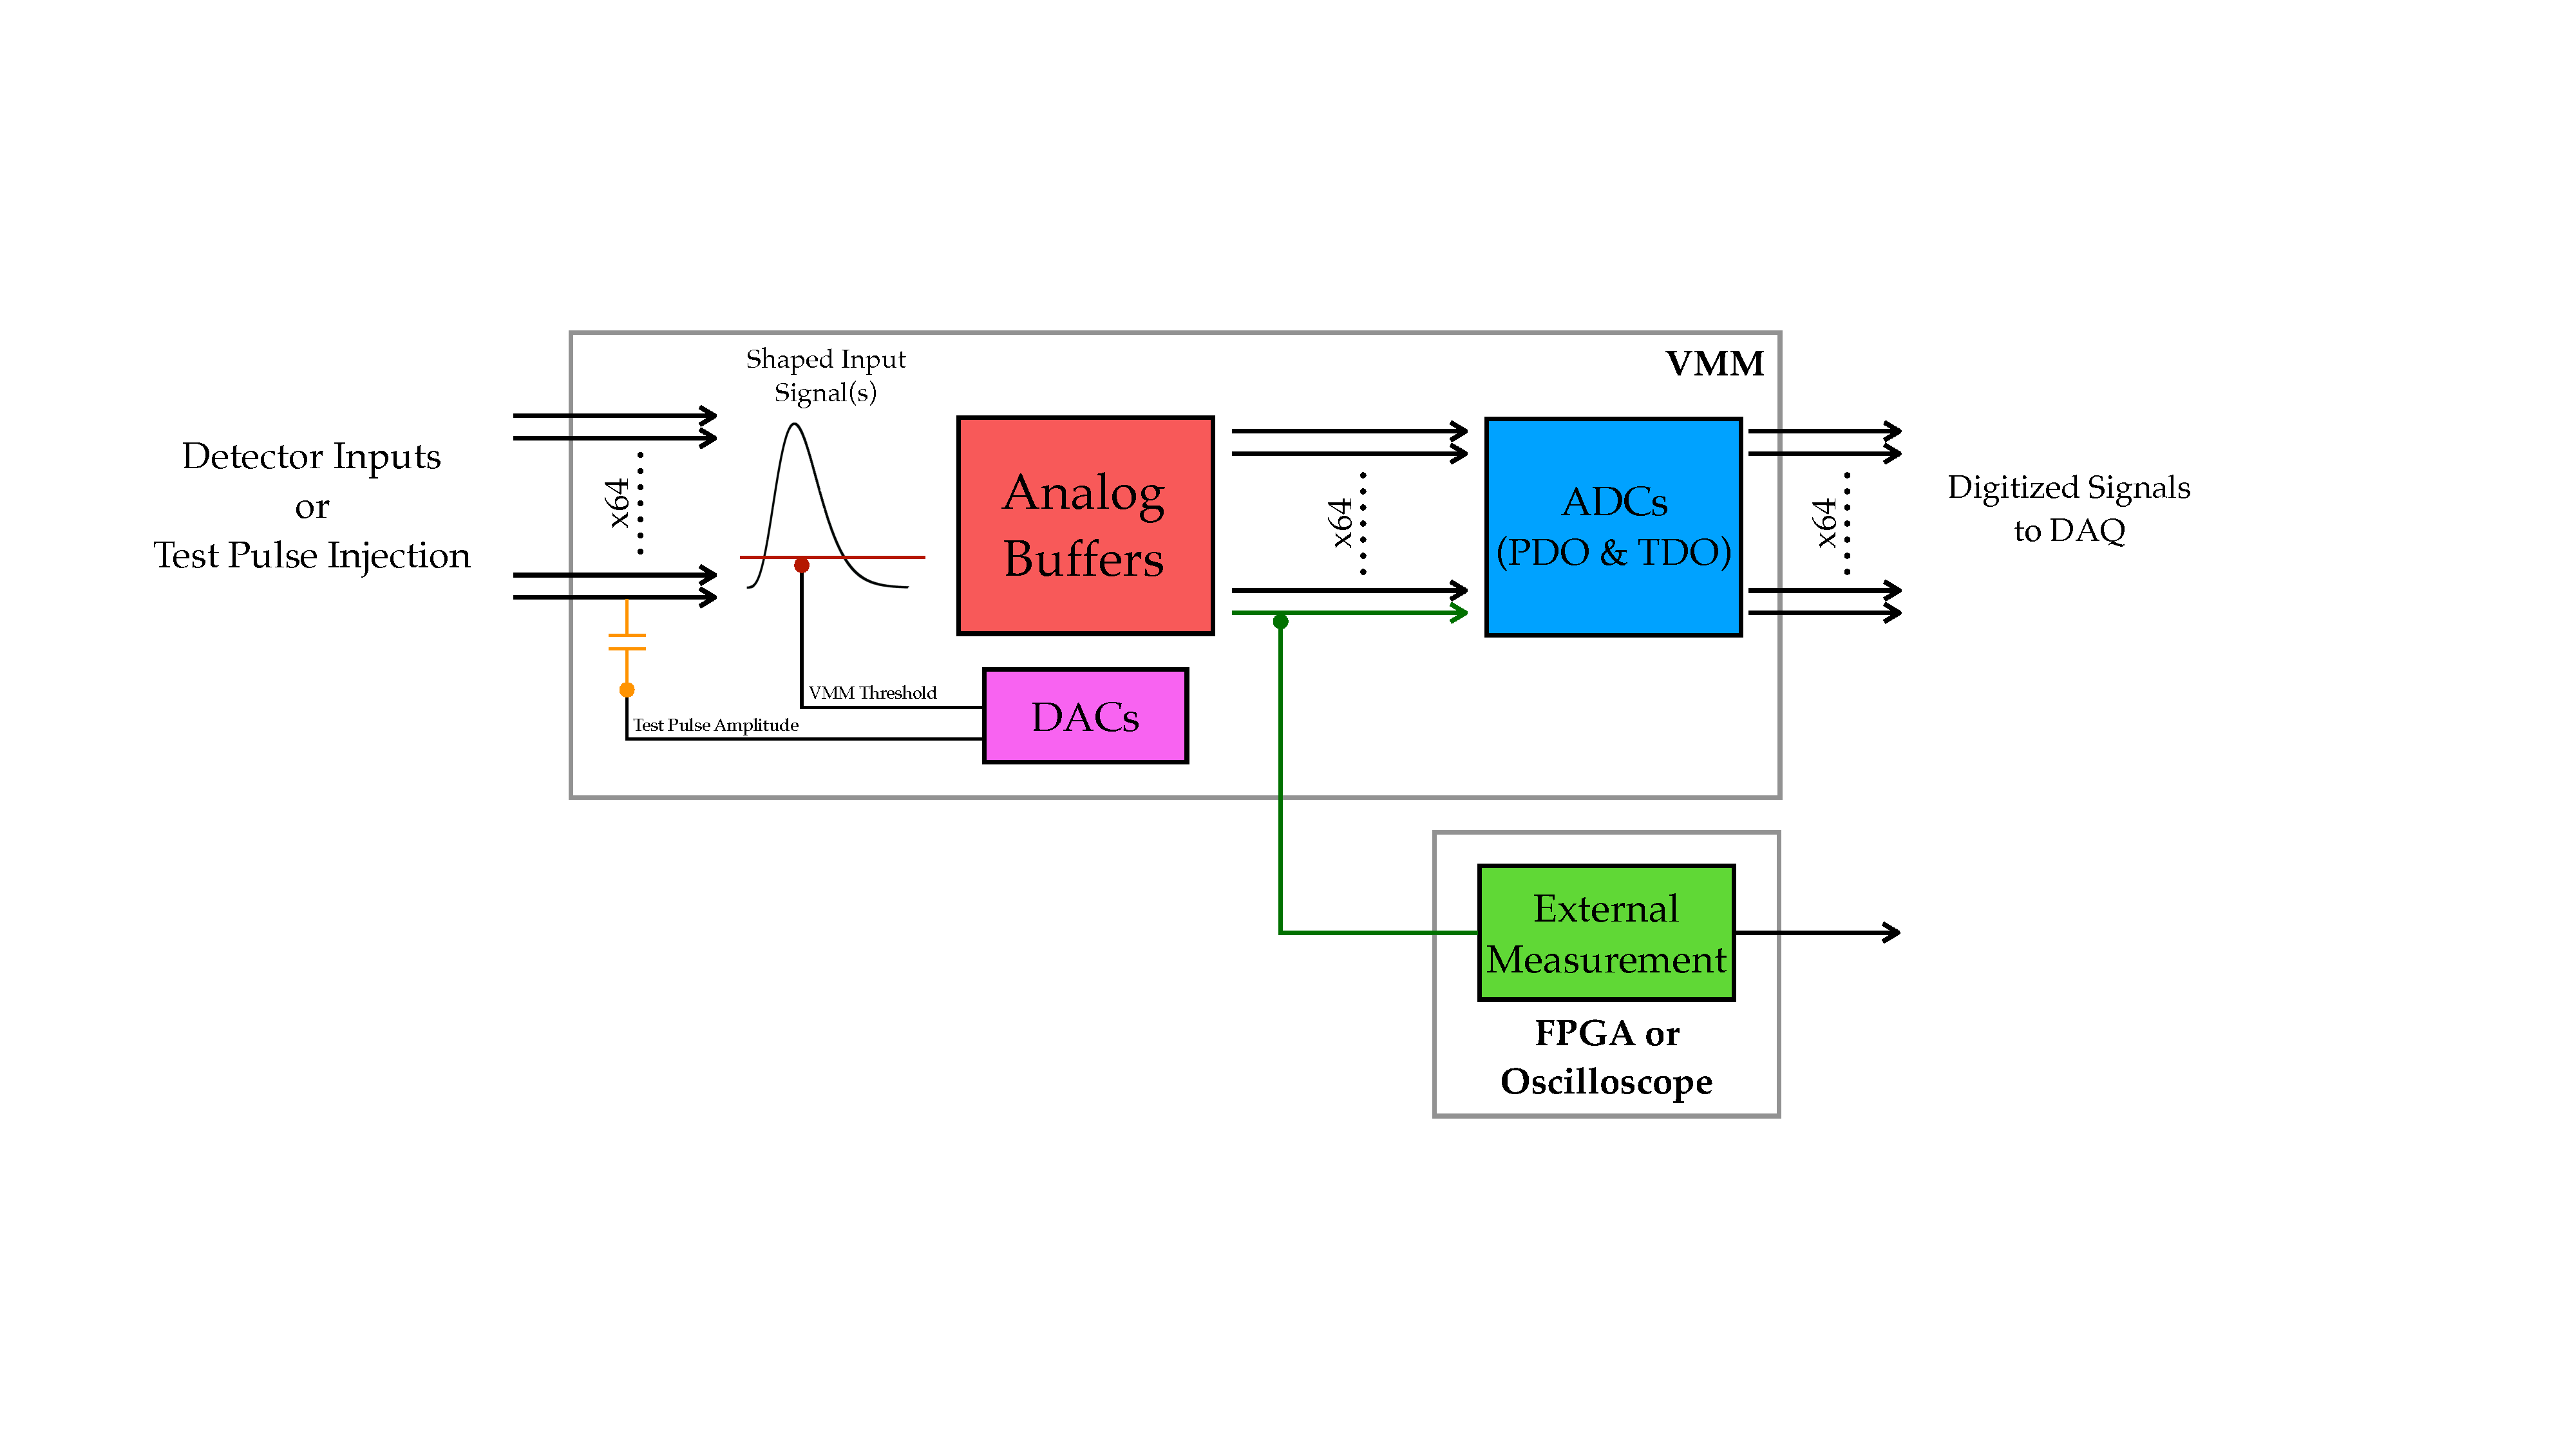
\includegraphics[width=0.8\textwidth]{figures/nsw/calibration/xadc_diagramPDF}
        \caption{
        }
        \label{fig:xadc_diagram}
    \end{center}
\end{figure}

As mentioned above, the VERSO software performs automated calibrations of
the frontend electronics.
The types of signals being collected on the NSW detectors are characterised by
very low signal amplitudes and are therefore typically noise dominated, with
much of the noise component derived mainly from the frontend electronics themselves.
It is therefore necessary to optimise the readout functionality of the
the VMM ASIC by calibrating it and ensuring that its signal-to-noise
ratio, $S/N$, is maximised during datataking.
Additionally, to achieve the best performance in the reconstruction of particle
tracks in the NSW detectors, several key aspects such as the charge amplitude
and timing measurement of the VMM need to be understood and well calibrated.
In this section a few of the calibration routines supported by VERSO will be discussed.

Many of the VMM calibrations rely on an external measurement of certain VMM characteristics
to be made.
These measurements are made using absolute measurements independent of any of the
internal VMM measurement mechanisms.
The VMM has built-in multiplexing capabilities that allow for it to route analog signals
to the MO output described in previous sections.
Specific for calibration, the VMM can route to MO any of the following:
\begin{description}
    \item[] \textbf{Channel Analog Output}: Analog levels of each channel's analog level prior to digitisation via the internal ADCs
    \item[] \textbf{Threshold DAC}: Analog output of the DAC controlling the global VMM threshold
    \item[] \textbf{Test Pulse DAC}: Analog output of the DAC controlling the test pulse amplitude
    \item[] \textbf{Channel Threshold Trimmers}: Analog measurement of each channel's discriminator's threshold voltage
\end{description}
On the frontend boards housing an FPGA, as in Figure~\ref{fig:frontend_boards}, the external measurement
is made by routing the MO output of a VMM to the built-in 12-bit ADC of the \textsc{Xilinx} FPGA, referred to as
the xADC.
The xADC has a full scale range of 1\,V, providing a digital measurement resolution of roughly 0.24\,mV.
The digitised samples produced by the analog measurements of the xADC are forwarded to the VERSO
DAQ software so that they can be stored and subsequently processed by the calibration algorithms.
As the xADC is housed in the on-board FPGA, the VERSO software can control its operation and access its measurements
using similar configuration and DAQ functionalities as described in the previous section.
Alternatively, the external measurement of the MO can be made via an oscilloscope probe.
The use of the oscilloscope probe does not lend itself to automated calibration but provides for
direct inspection of the analog levels as well as a reference on the measurements of the xADC.
An illustration of these external measurement mechanisms is provided in Figure~\ref{fig:xadc_diagram}.

\subsubsection{DAC Calibration}
\label{sec:calib_dac}

Each VMM has two important DACs: one for setting the global VMM threshold and one for
setting the amplitude of the injected test-pulse charge via the test-pulse capacitor on each
channel.
Each is 10-bit, meaning that it can be set to a value of 0-1023 (inclusive).
In order for the user to know in absolute terms what the VMM threshold or test-pulse amplitude
is set to, i.e. in terms of analog voltage values and not digital counts, the analog level of each
DAC is measured using the xADC.
At each configured DAC value, between 0 and 1023, analog measurements are made of the DAC output and
the relationship between the output analog value and configured digital value can be obtained.
This is illustrated in Figure~\ref{fig:threshold_dac_calib} for a single VMM's threshold DAC.
A linear relationship is assumed and from a linear fit the \textit{DAC-mV} relation, giving
the mapping from the configured digital DAC value to its analog value observed by the VMM channels, is obtained
from the slope of the line.
The DAC-mV relation between VMMs is not necessarily the same, and therefore must be measured
for every single VMM in the system in order to be able to configure them all with the
same \textit{absolute} threshold or to inject test pulses with common amplitudes across VMMs.
Given the known capacitance of the test-pulse injection capacitor of the VMM channels,
the value of the injected charge for a configured test-pulse amplitude can be obtained via the $Q = C \cdot V$
relation, where $C$ is the injection capacitor's capacitance and $V$ is the test-pulse DAC output amplitude.%\footnote{
%The quoted capacitance value of the VMM channel's test-pulse injection capacitor, 3\,pF, is that of the
%VMM3 series of VMM. Earlier versions had lower capacitances.
%}

\begin{figure}[!htb]
    \begin{center}
        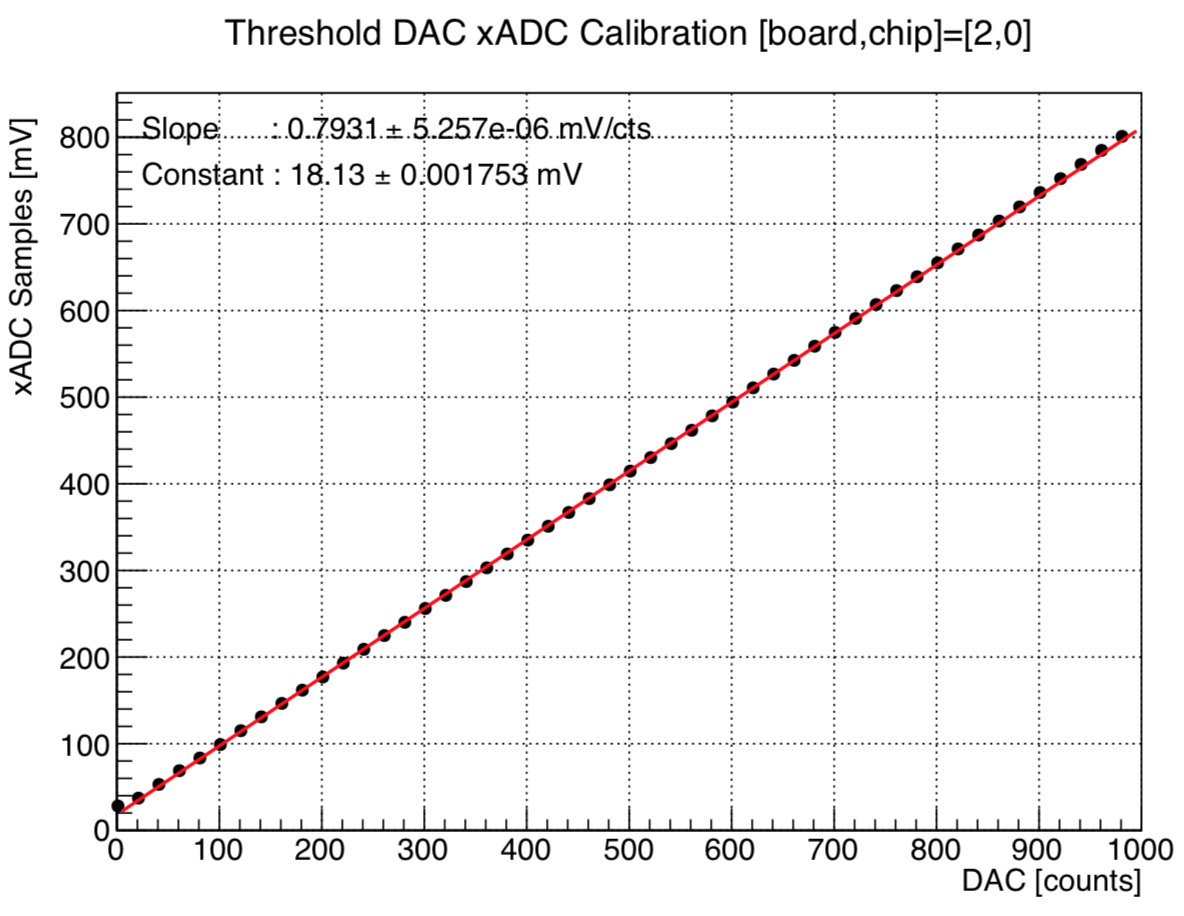
\includegraphics[width=0.6\textwidth]{figures/nsw/calibration/threshold_dac_calib}
        \caption{
            VMM global threshold measurement, using measurements made by the xADC, as a function
            of the set digital DAC value.
            The slope and y-intercept (`Constant') of the linear fit are provided.
            The slope gives the DAC-mV relation that allows for converting the digtal DAC
            configured value to an analog level at the VMM inputs.
        }
        \label{fig:threshold_dac_calib}
    \end{center}
\end{figure}

\subsubsection{Measurement of Channel Baselines and Noise}
\label{sec:calib_baselines}

External measurements via the xADC can be made of each channel's analog output (i.e. prior
to digitisation) when no signals are present at the channel input.
Doing so allows one to obtain a measurement of the channel \textit{baseline}, i.e. the
ambient level when no signal is present.
Fluctuations about the baseline, then, give a measurement of the inherent channel \textit{noise}.
Measurements of both of these quantities are important, both when the frontend electronics
are and are not interfaced to a detector.
Measurements of the noise when the frontend electronics are not interfaced to a detector give
a measurement of the inherent electronics noise characteristic of the frontend board.
Interfacing the frontend electronics to a detector introduces additional capacitive effects
that can introduce new sources of noise that must also be studied and reduced.
Knowledge of both the absolute baseline and noise levels of each VMM allows for the optimal threshold
to be set for each.
In order to be sensitive to small-amplitude signals, one would set the threshold just above the baseline
which sets the zero-level of an observable signal.
In practice, one sets the VMM threshold a few times the magnitude of the measured noise above the baseline: typically
2 to 3 times the level of the measured noise above the baseline.
Figure~\ref{fig:baselines_calib} shows an example of the measurements of a VMM channel's baseline and noise, taken by the xADC.
The xADC samples each channel's baseline and from the width of the distribution of these measurements the noise
level can be obtained.

\begin{figure}[!htb]
    \begin{center}
        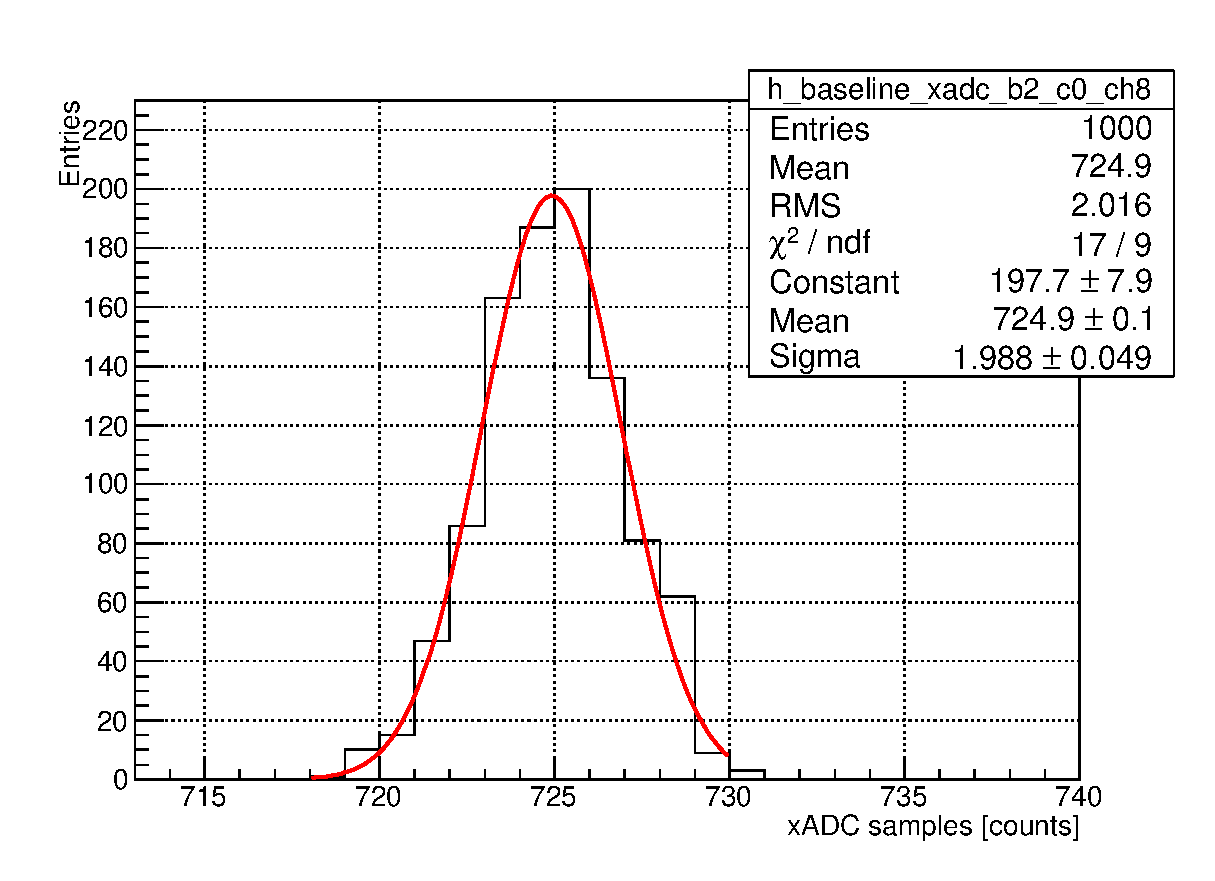
\includegraphics[width=0.46\textwidth]{figures/nsw/calibration/xadc_calib_channel_baseline_samples}
        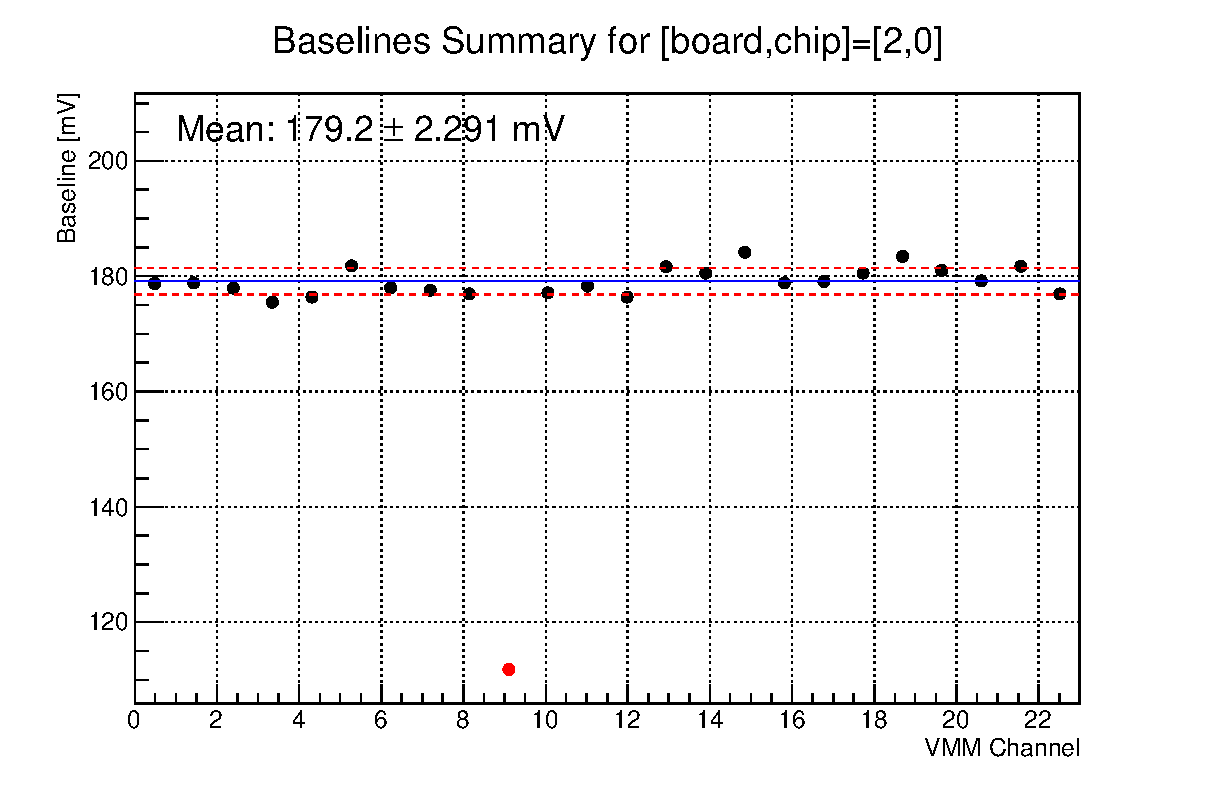
\includegraphics[width=0.53\textwidth]{figures/nsw/calibration/calib_baselines_vmm_summary}
        \caption{
            \textbf{\textit{Left}}: 1000 xADC measurements of a single VMM channel's input baseline.
                The width of the gaussian fit (red) gives the channel's noise level.
            \textbf{\textit{Right}}: Summary of the baseline measurements for 24 channels of a VMM.
                The error on the reported mean baseline, which is indicated by the blue line, is given by the RMS spread of the baseline measurements
                across all channels and is indicated by the red dashed lines.
                The channel with the red point (channel 9) is a faulty (dead) channel.
        }
        \label{fig:baselines_calib}
    \end{center}
\end{figure}

\subsubsection{Channel Threshold Trimming}
\label{sec:calib_trimming}

The global VMM threshold inherently has channel-to-channel variation.
In order to ensure that the VMM discriminators of all channels in the system
fire at the same value, the VMM has a per-channel threshold trimming functionality included.
This functionality allows for each channel's threshold to be adjusted (`trimmed') in 32 steps that cover a range
of approximately 32\,mV.
To equalize the channel discriminators, external measurements made via the xADC are performed.
For each channel, measurements of the channel discriminator's threshold are taken at each of the 32
steps in the allowed range of trimming.
Once done for every VMM channel in the system, a metric for equalizing their thresholds is needed.
In the example of Figure~\ref{fig:calib_channel_trim}, the metric is to bring all channels
as close as possible to the globally set VMM threshold.
Once this is done, all VMM channels in the system ideally have equal thresholds and will
have equivalent responses to input signals.
As seen in Figure~\ref{fig:calib_channel_trim}, prior to this calibration there is quite
some variation, which shows the importance of this fine-grained calibration procedure.
The amount of threshold trimming necessary to bring a channel to its equalized state
is independent of the globally set VMM threshold; therefore, once the calibration procedure
is performed and the subsequent channel threshold trimming is applied, the global
threshold can be adjusted with confidence that all channels in the system are likewise adjusted coherently.

\begin{figure}[!htb]
    \begin{center}
        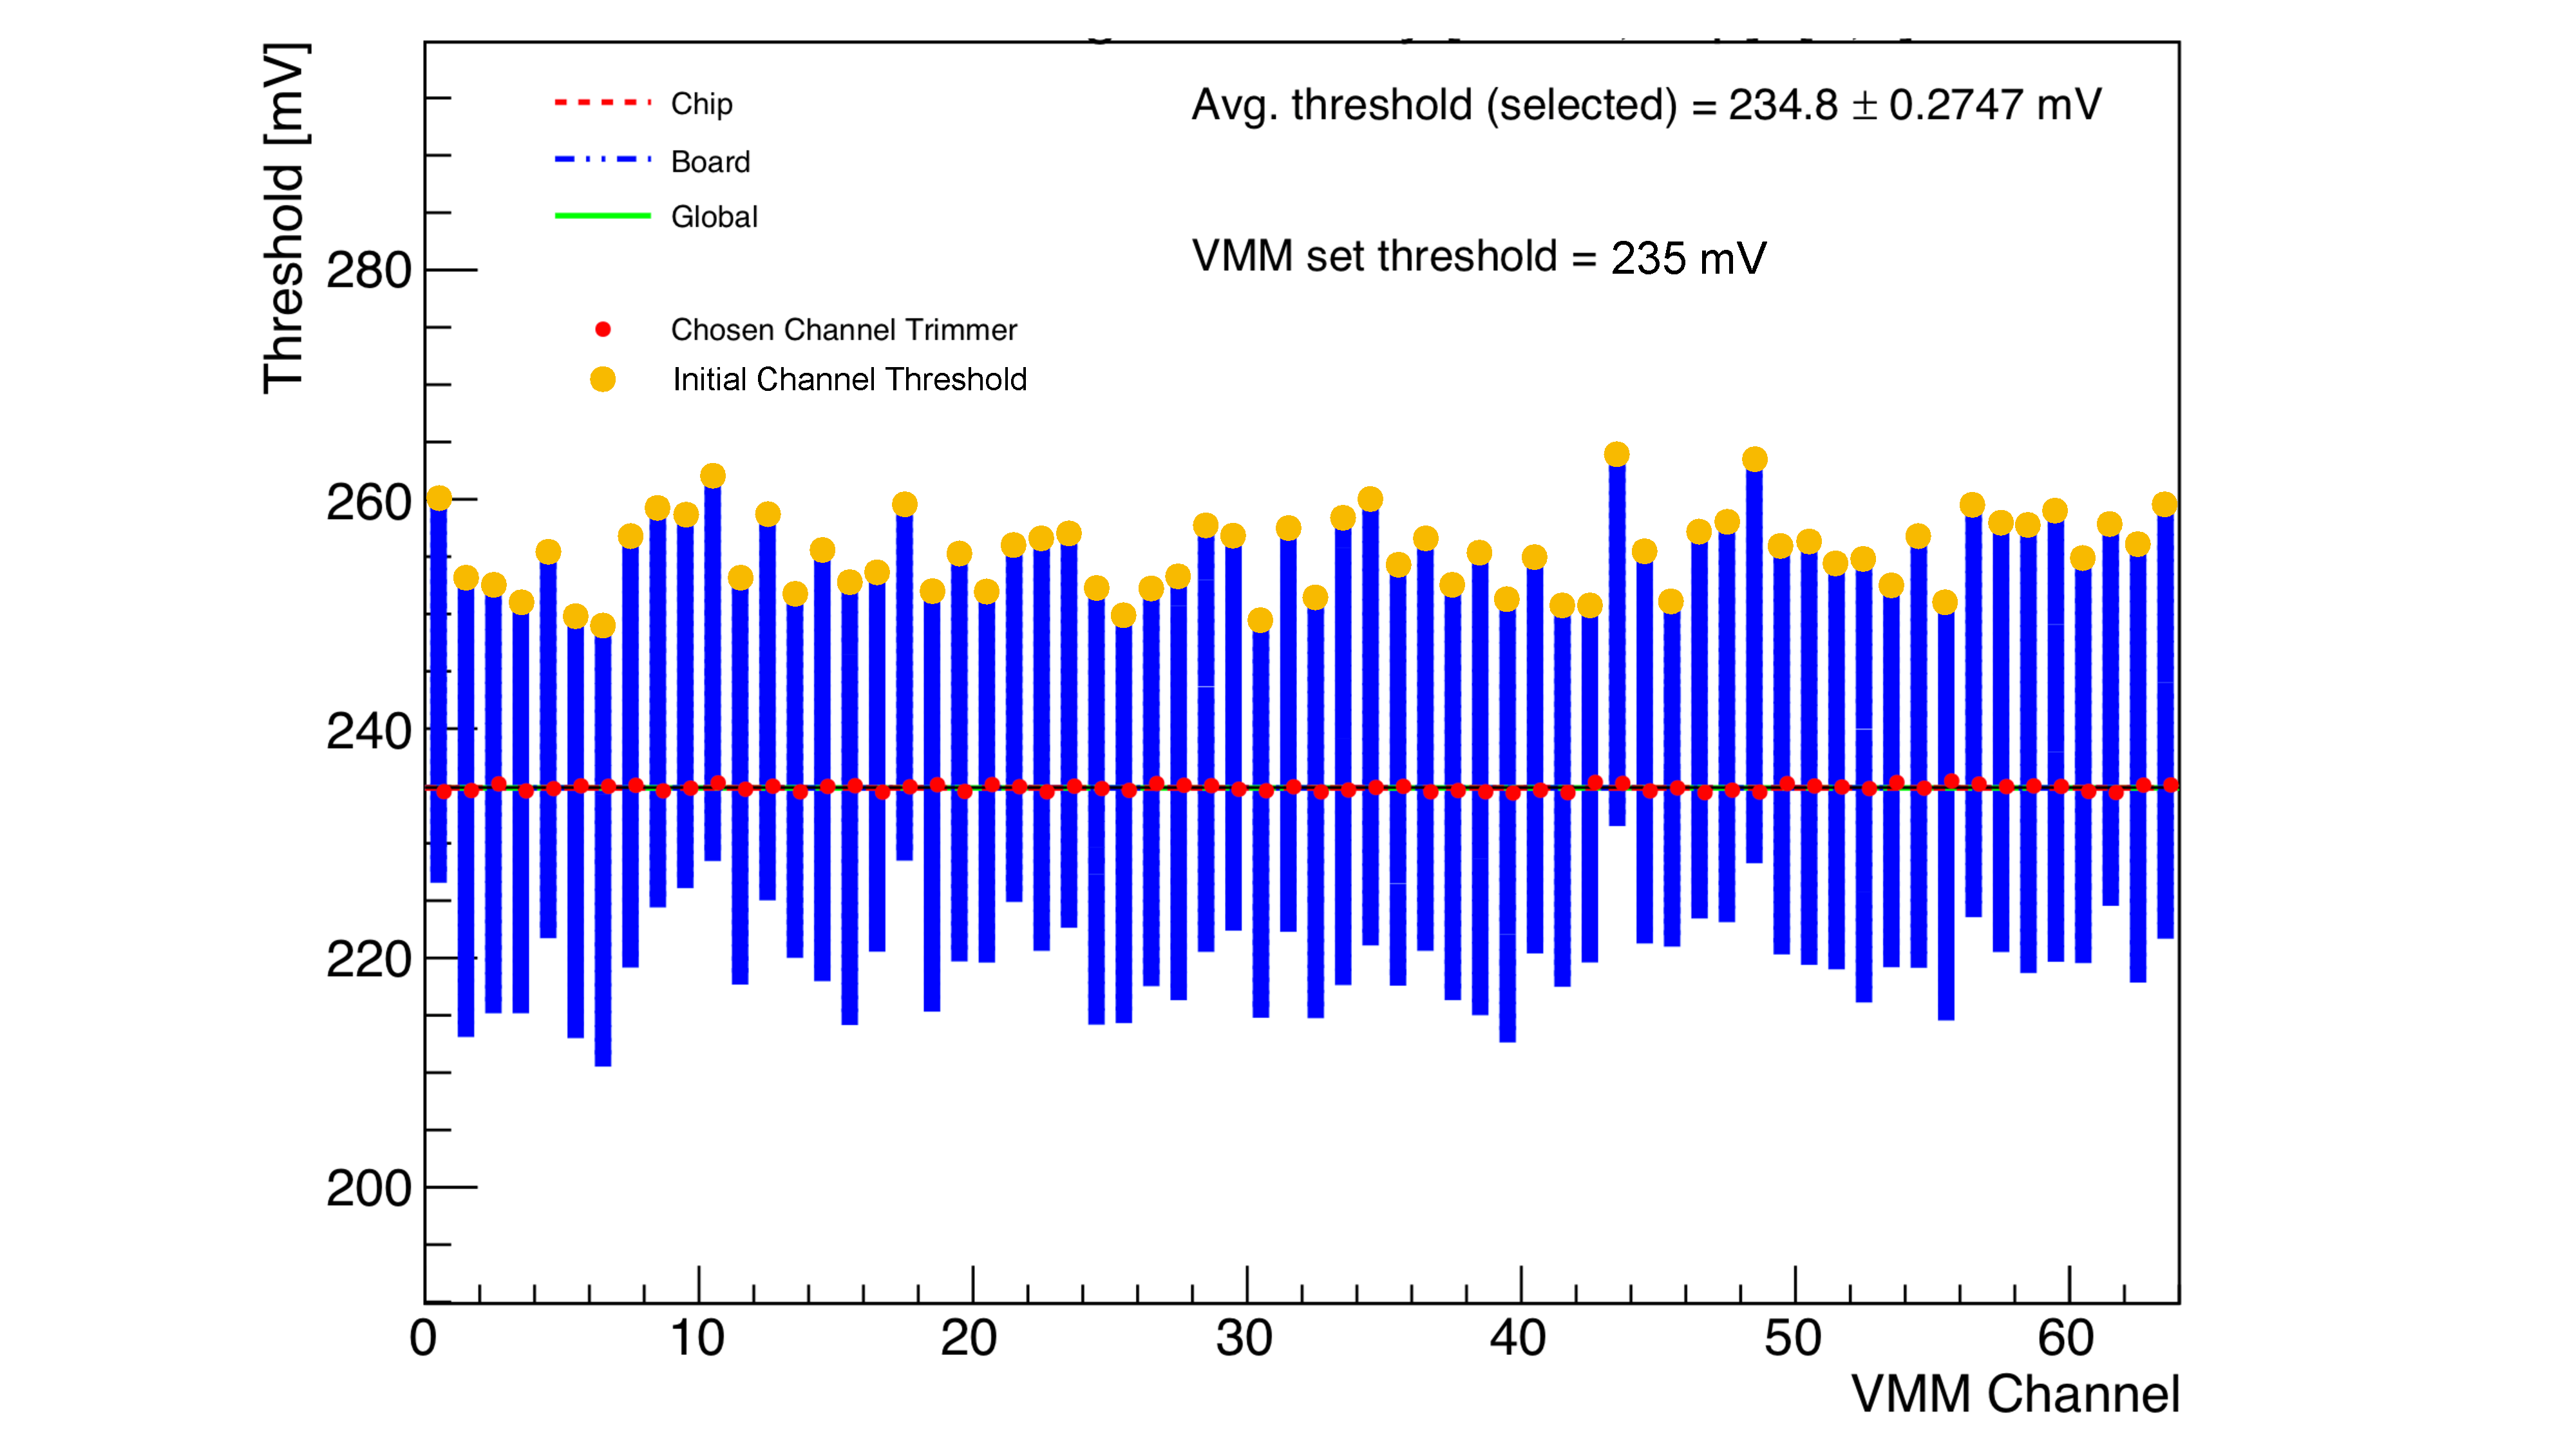
\includegraphics[width=0.85\textwidth]{figures/nsw/calibration/channel_threshold_calibPDF}
        \caption{
            Summary plot of a VMM channel threshold trimming calibration.
            For this set up, a single VMM is calibrated and has a global threshold
            set to 235\,mV.
            The channel-by-channel variation of the threshold is seen by the yellow dots,
            which indicate the per-channel threshold measurement made by the xADC prior to any
            threshold trimming.
            The blue columns indicate the entire threshold range accessible by each channel
            by scanning the full range of channel trimmers and taking xADC measurements at each.
            It can be seen that most channels have a full range of approximately 32\,mV.
            The calibration algorithm shown here picks for all VMM channels the amount of trimming
            that allows for them to have thresholds as near as possible to the globally set threshold.
            In this case, the post-calibration threshold of all channels, indicated by the red dots,
            is very nearly 235\,mV, and is $234.8\pm 0.27$\,mV on average.
        }
        \label{fig:calib_channel_trim}
    \end{center}
\end{figure}

\subsubsection{Signal Amplitude Gain and Pedestal}
\label{sec:calib_pdo}

\subsubsection{Timing Measurement Calibration}
\label{sec:calib_tod}


\FloatBarrier

%%%%%%%%%%%%%%%%%%%%%%%%%%%%%%%%%%%%%%%%%%%%%%%%%%%%%%%%%%%%%%%%%%%%%%%
% VERSO USE CASES
%%%%%%%%%%%%%%%%%%%%%%%%%%%%%%%%%%%%%%%%%%%%%%%%%%%%%%%%%%%%%%%%%%%%%%%
\subsection{Use Cases}
\label{sec:verso_use_cases}

Throughout the timespan of the present thesis, the VRS and, specifically, the VERSO software infrastructure
has been used in a wide variety of settings and for many purposes.
In this section a few such use-cases will be highlighted.

\subsubsection{Test Benches}
\label{sec:verso_test_bench}

For the majority of studies of the frontend electronics, namely the frontend boards
and the VMM ASIC, detectors are not needed.
For this reason, one of the primary uses of the VRS and VERSO DAQ and calibration software
is in testbenches in electronics labs.
A typical setup is shown in Figure~\ref{fig:vrs_testbench}.
The use of VRS in the testbench allows for quick and direct inspection
of the frontend electronics via an oscilloscope.
In such a setup, the response of the frontend electronics to communications sent
from VERSO to the FGPA (or the FPGA to the VMM), and vice versa, can immediately be seen
by visual means.
Calibration and off-detector performance of the frontend electronics and VMM can also be studied
in the `clean' scenarios provided by the testbench setup.
Use in labs and testbenches has allowed for the VRS software and firmware to be fully validated and for
the validation of the NSW frontend boards as they have evolved.

\begin{figure}[!htb]
    \begin{center}
        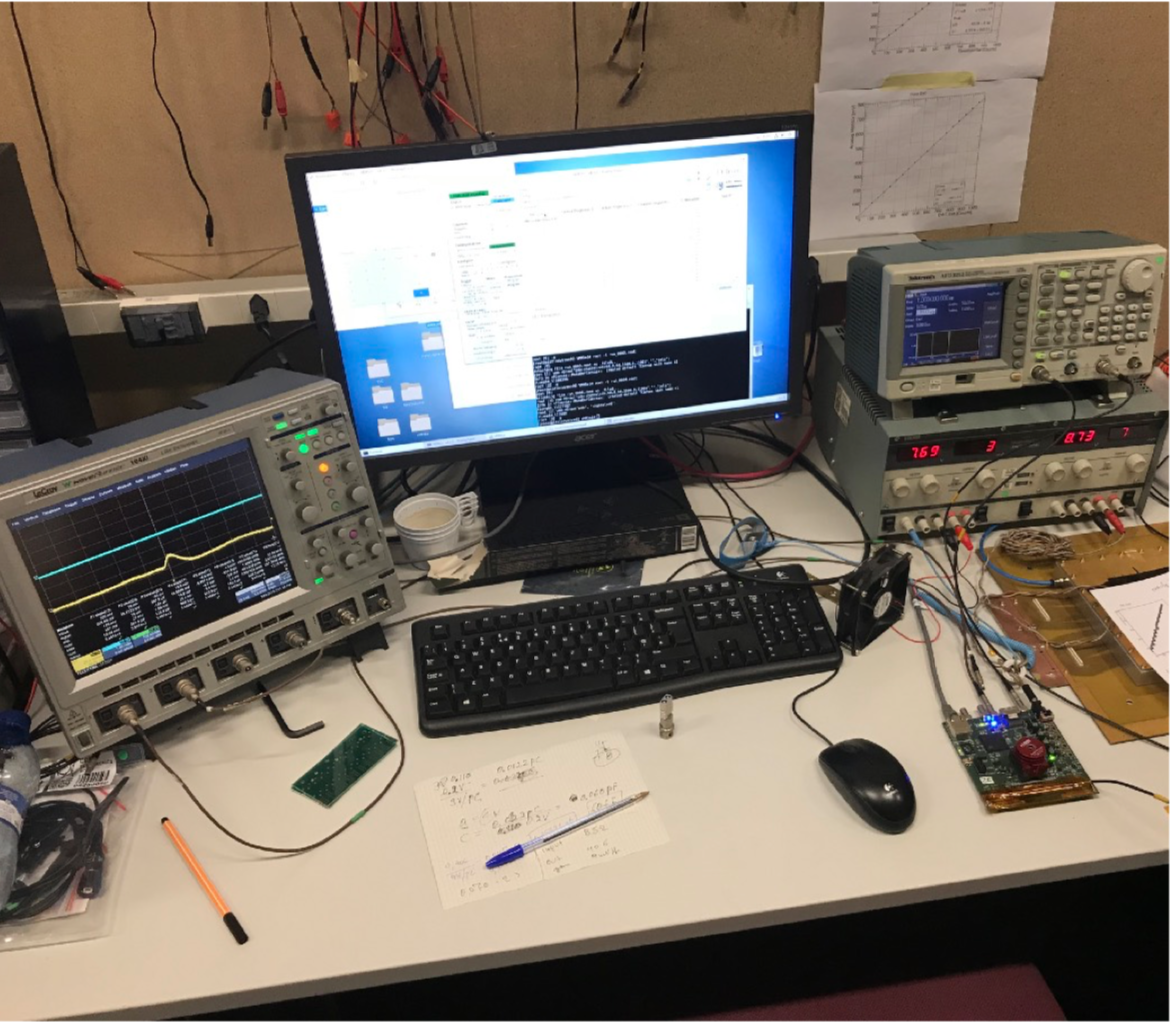
\includegraphics[width=0.49\textwidth]{figures/nsw/use_cases/verso_use_case_vs_socket}
        \raisebox{0.28cm}{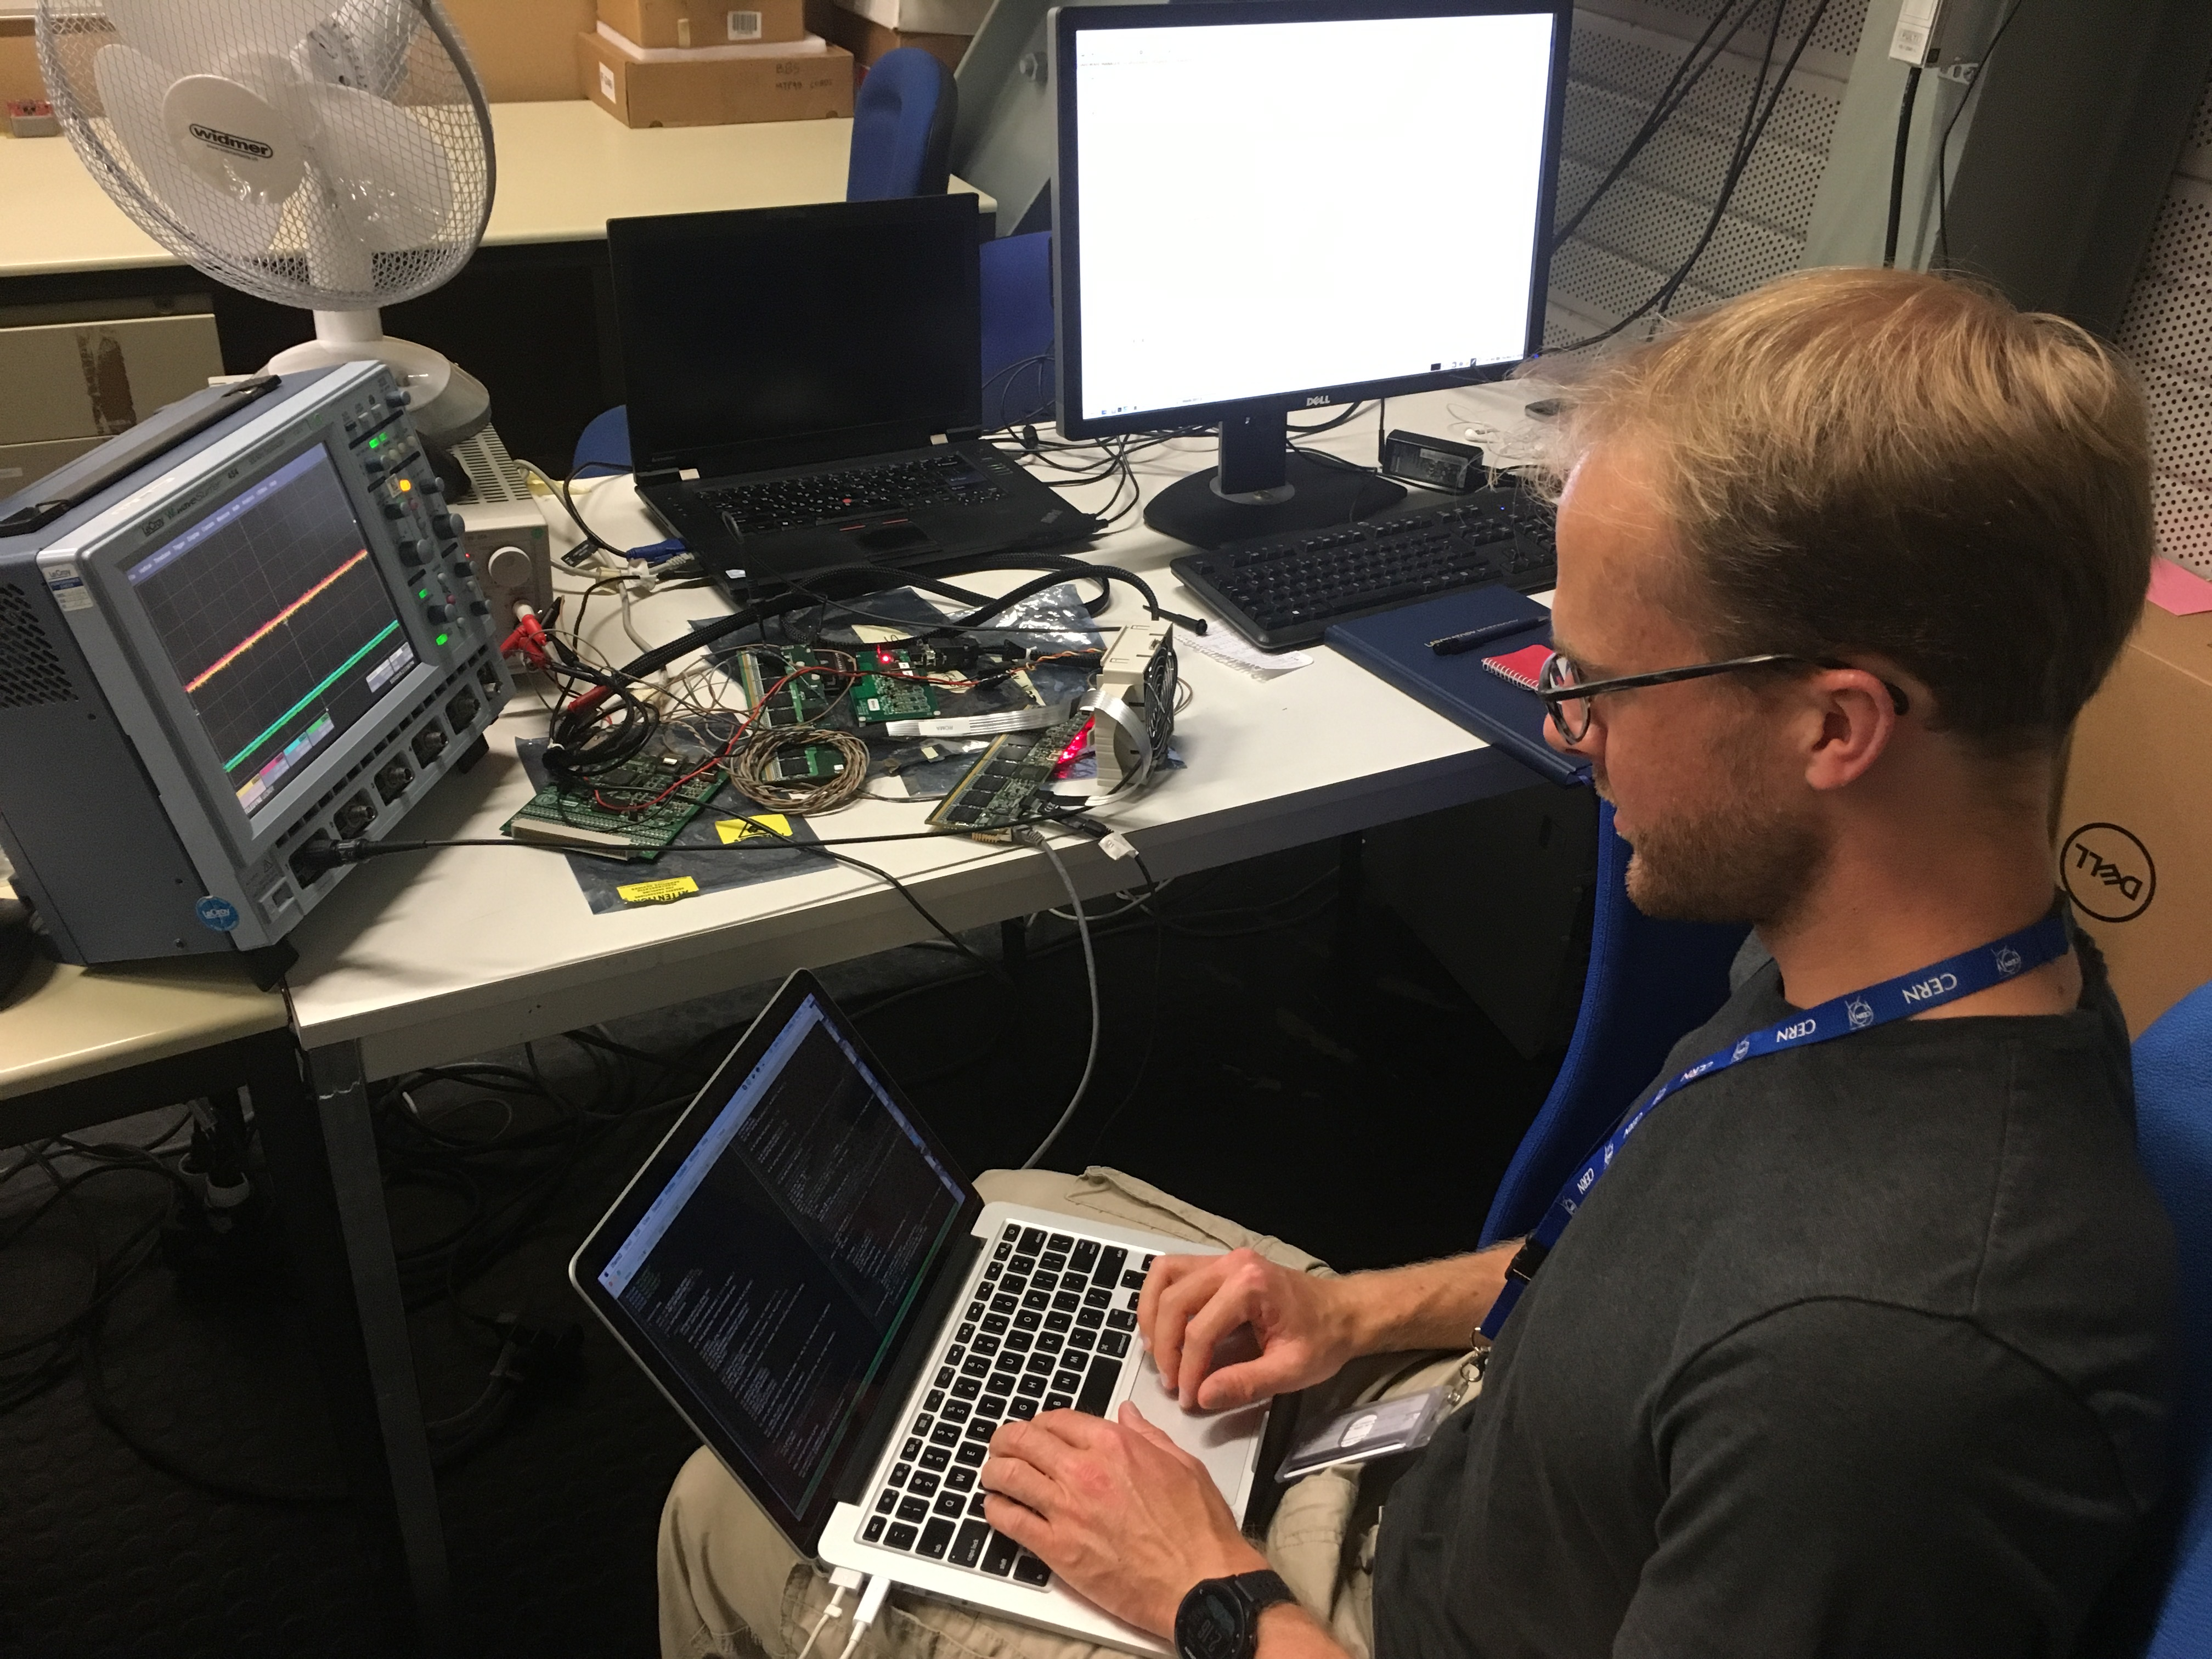
\includegraphics[width=0.49\textwidth]{figures/nsw/use_cases/vrs_dantrim}}
        \caption{
            \textbf{\textit{Left}}: A typical VRS testbench setup.
                The frontend board housing the VMM is seen in the picture on the lower right (GPVMM-type frontend board).
                An oscilloscope is available for probing the frontend board and VMM outputs visually.
                The frontend board is connected to the shown PC via a direct Ethernet connection.
                A function generator producing input signals is at the right, being used to test the injection
                of signals independently from the VMM channel test charge capacitors.
            \textbf{\textit{Right}}: Another example of a typical testbench setup, with the present
                author hard at work.
                In this case, VERSO is hosted on a single laptop with a direct Ethernet connection to the frontend board.
                The frontend board in this case is an MMFE8-type frontend board.
                In the case shown, the VRS firmware on the frontend board is being debugged.
                The PC at the upper right, connected to the frontend board via a mini-SAS connection, is responsible for writing and uploading the firmware to the
                on-board FPGA.
        }
        \label{fig:vrs_testbench}
    \end{center}
\end{figure}

\subsubsection{Cosmic Stand}
\label{sec:verso_cosmic}

The VRS system has also been used to collect cosmic muon data from instrumented detectors, on cosmic stands
located in NSW labs at CERN and elsewhere.
One such example is shown in Figure~\ref{fig:mm_quad_elx}, showing the large-scale MM chambers
in the cosmic stand located at the RD51 lab at CERN.
Another, more recent (at the time of writing) example is that of the final MM detector integration
site whereat the final NSW MM chambers are being assembled.
As the final DAQ system that will be used once the NSW is installed in ATLAS is not yet fully ready,
at the time of writing, the VRS system was used to configure and readout the frontend electronics
interfaced to the final full-scale MM double-wedges.
For the final integration, noise tests of the electronics on the final MM detectors that will be
installed in ATLAS are needed in order to verify the base performance of the large-scale detectors.
The double-wedge MM detectors are additionally placed onto a cosmic-ray stand and initial data was able to be
collected with the VRS and VERSO DAQ software.
The VRS system, in this case, helped allow for the final NSW MM integration procedures to be put into place
while the full-scale DAQ infrastructure to be used once the NSW is installed in ATLAS was made available.

\begin{figure}[!htb]
    \begin{center}
        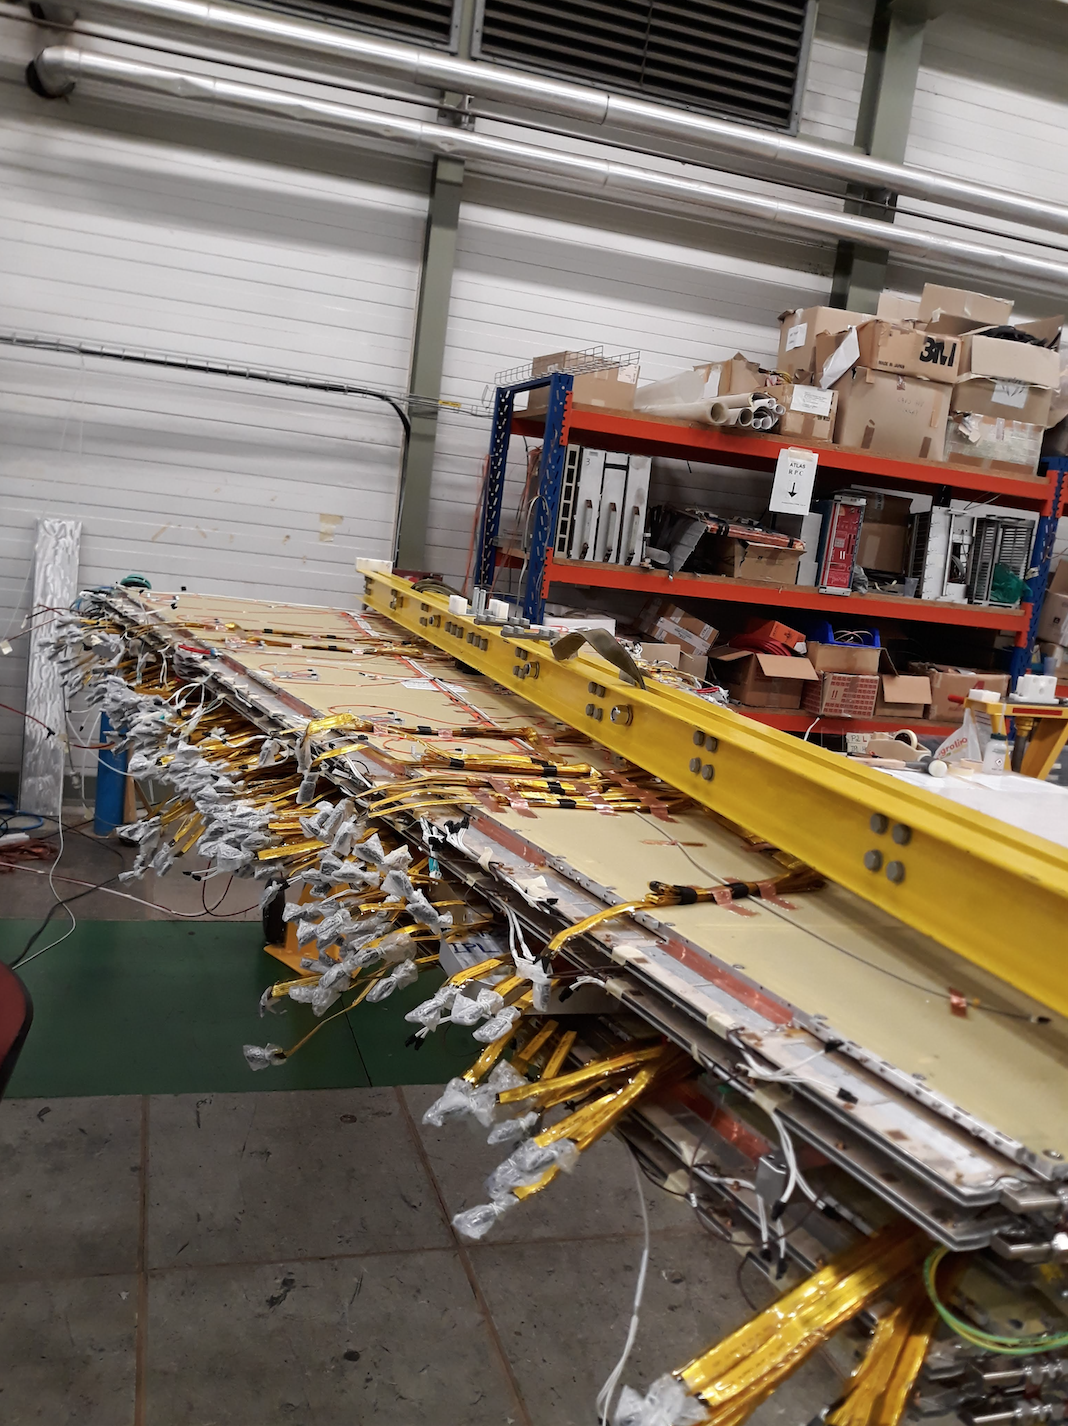
\includegraphics[width=0.48\textwidth]{figures/nsw/use_cases/mm_bb5}
        \raisebox{2.5cm}{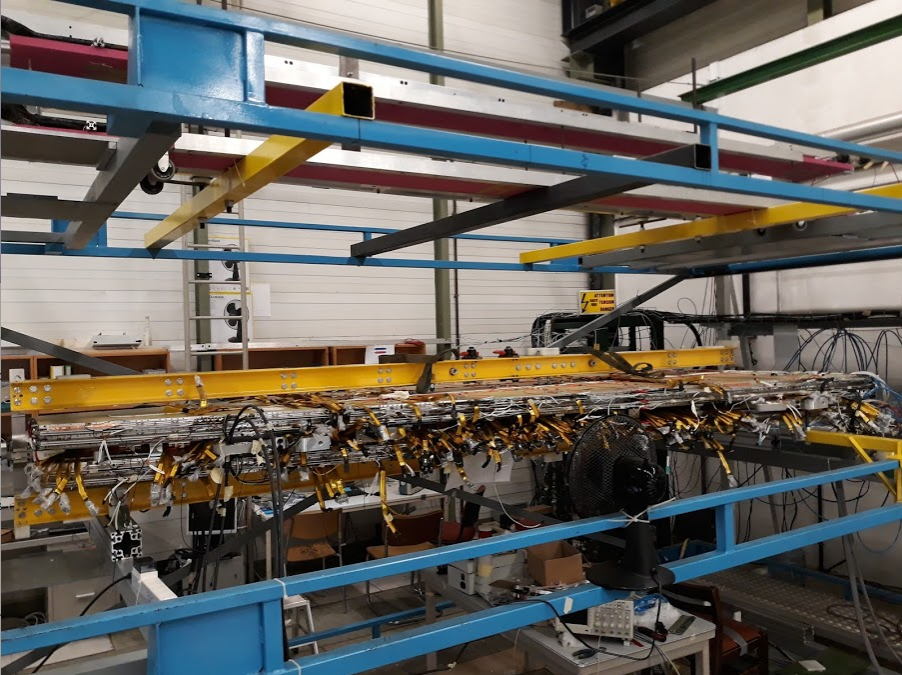
\includegraphics[width=0.48\textwidth]{figures/nsw/use_cases/mm_bb5_cosmic}}
        \caption{
            \textbf{\textit{Left}}: Assembled NSW MM sector (double-wedge) at the MM integration
                site at CERN.
            \textbf{\textit{Right}}: MM sector on the cosmic-ray test-stand at the MM integration site
                at CERN. The detector is instrumented with MMFE8 frontend boards with Ethernet readout
                achieved via the VRS and VERSO DAQ software, hosted on the PC located just behind the cosmic
                stand.
        }
        \label{fig:mm_bb5}
    \end{center}
\end{figure}


\subsubsection{Frontend Board Validation}
\label{sec:verso_noise}

The design of the frontend board to be used in the NSW was being finalised throughout the timespan
of this thesis.
In order to validate that the frontend board met the standards required for operation in the NSW, specifically
that it did not introduce too much electronics noise as a result of its design,
the VRS system and VERSO software were required.
The prototype boards, then, for the NSW are all outfitted with an FPGA and Ethernet connector as in Figure~\ref{fig:frontend_boards}
so that they can be interfaced with the VRS readout system.
The main goals of the frontend board validation are to ensure proper routing between the VMM
ASIC and the rest of the frontend board elements which can be tested by verifying the VMM's response
to specific configuration commands.
Noise tests are also performed by measuring the frontend board noise as described in Section~\ref{sec:calib_baselines}.
Such an example of a noise tests using prototype MMFE8s while interfaced to full-scale MM detector chambers
is shown in Figure~\ref{fig:mm_quad_elx}.
Performing such tests allow, also, to verify that the physical connections between the frontend electronics and detectors, such as the ZEBRA connectors in the
case of the MM detectors,
are without fault. Any such fault would appear as a faulty set of channels only when the electronics
are interfaced to the detector, for example.

\subsubsection{Testbeams}
\label{sec:verso_testbeam}

\begin{figure}[!htb]
    \begin{center}
        \raisebox{1.8cm}{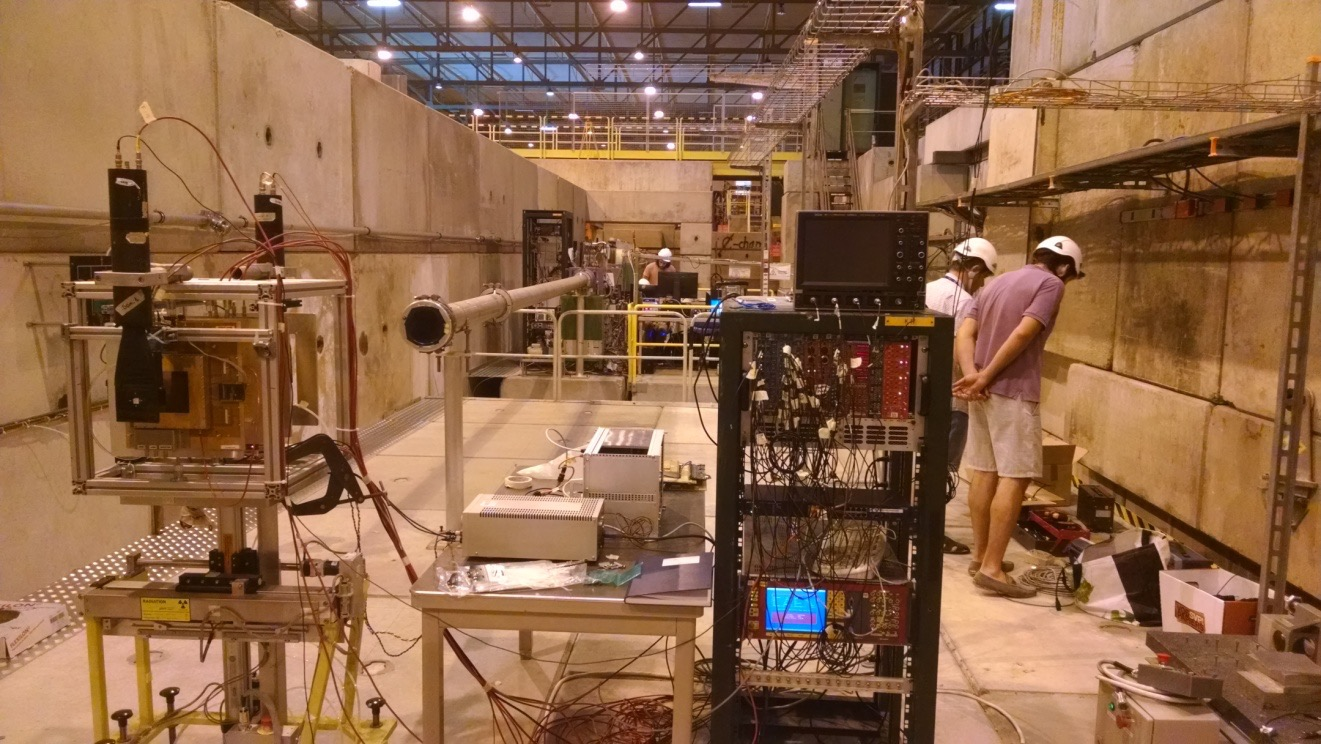
\includegraphics[width=0.58\textwidth]{figures/nsw/use_cases/vrs_testbeam}}
        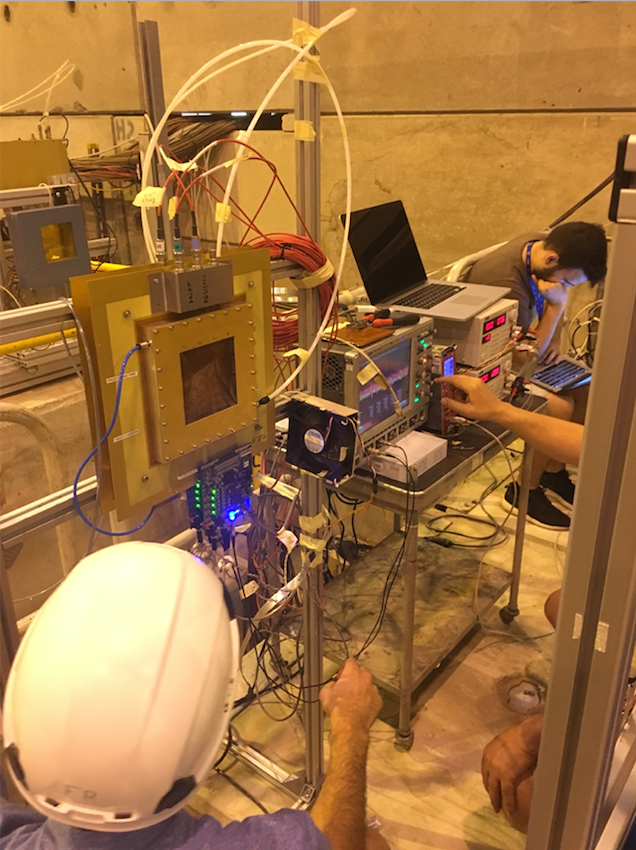
\includegraphics[width=0.4\textwidth]{figures/nsw/use_cases/verso_testbeam2}
        \caption{
            \textbf{\textit{Left}}: Typical testbeam setup at the CERN North Area, located at the Prevessin Site at CERN.
                The small prototype MM chambers are housed in the aluminum frame on the left with scinitllator
                trigger paddles on either side.
                The beam tunnel can be seen extending into the distance.
                The trigger and high voltage systems are seen on the rack in the middle of the picture.
                The DAQ PC is housed in a control room (not shown) some 10-15\,m outside of the beam area.
            \textbf{\textit{Right}}: A close up of a small prototype MM chamber at a test beam. The
                GPVMM-type frontend board is interfaced at the bottom. Here it can be seen that there
                are two MM chambers back-to-back, each with a frontend board attached at their bottom.
                The cables providing high voltage (in red) and gas (white) to the MM chambers are seen, as well.
        }
        \label{fig:vrs_testbeam}
    \end{center}
\end{figure}

From 2016 until the present time of writing, the VRS system and VERSO DAQ software have been used as the main DAQ infrastructure
for test beam campaigns at CERN.
The testbeam area at CERN is located at the CERN Prevessin site, in the North Area.
Proton beams from the SPS are made to collide with a fixed target upstream of the detectors and
the collision products are sent through several beamlines in the North Area along which
detectors can be placed.
The beams from the SPS are extracted roughly every 40\,seconds and particles are sent down the beamlines towards
the detectors for roughly 5\,second `spills'.
In such cases, the particle rates observed at the detectors are on the order of several 100\,kHz.
The main purpose of these testbeam campaigns was to verify the performance of both the VMM ASIC and prototype NSW frontend
boards in high-rate environments.
The VRS system and VERSO DAQ software have succeeded in recording data at 100\% efficiency at these
rates, allowing for high volumes of data to be collected and used in NSW detector performance and electronics studies.
For such data, used to validate the frontend electronics and tracking performance of NSW-type detectors in realistic data-taking environments,
the calibration routines described in Section~\ref{sec:calib_alg}, and implemented within the VERSO software infrastructure, are of the utmost importance.

\subsubsection{VMM Production Validation}
\label{sec:verso_vmm_prod}

Throughout the work presented in this thesis, the VMM ASIC has gone through 3 versions.
In order to validate that a given VMM production is adequate --- meaning that there is no systematic
fault in the ASIC production, for example --- large scale tests of all ASICs produced in manufacturing test runs 
are required.
In many cases, the automated calibration routines supported by VERSO were required to perform these production
tests.
In one such case, the manufacturing process of the silicon wafers used to produce the VMM was changed
and in order to verify that the resulting changes observed on the VMM performance were due to this
change, a direct study of the VMM charactertics prior to the changed process being applied
to the silicon was needed.
This is shown in Figure~\ref{fig:vrs_vmm_prod}, in which a silicon wafer containing pre-cut and pre-thinned
VMM ASICs are being interfaced directly with the VRS and VERSO DAQ software.
The interfacing of the VERSO DAQ and calibration software is achieved by the use of a custom-made
adapter board provided to the silicon inspection machine, shown on the right side of Figure~\ref{fig:vrs_vmm_prod}, that makes all the necessary
connections to the VMM ASIC pins by making direct contact with the silicon.
The silicon wafer is moved beneath the adapter card via the inspection machine
so that it may inspect different locations on the silicon wafer in which the VMM ASICs are located.

\begin{figure}[!htb]
    \begin{center}
        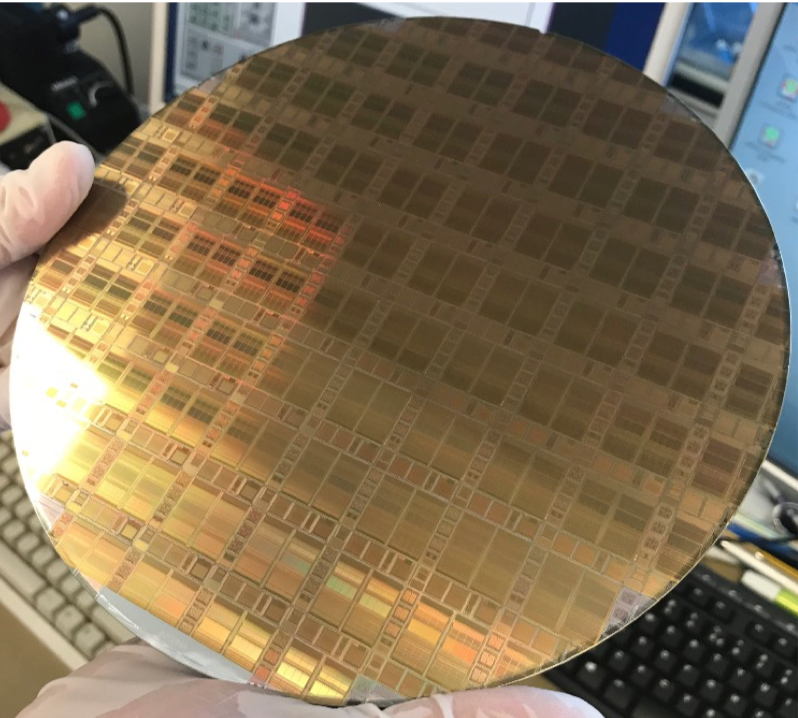
\includegraphics[width=0.49\textwidth]{figures/nsw/use_cases/verso_use_case_vmm_die}
        \raisebox{0.85cm}{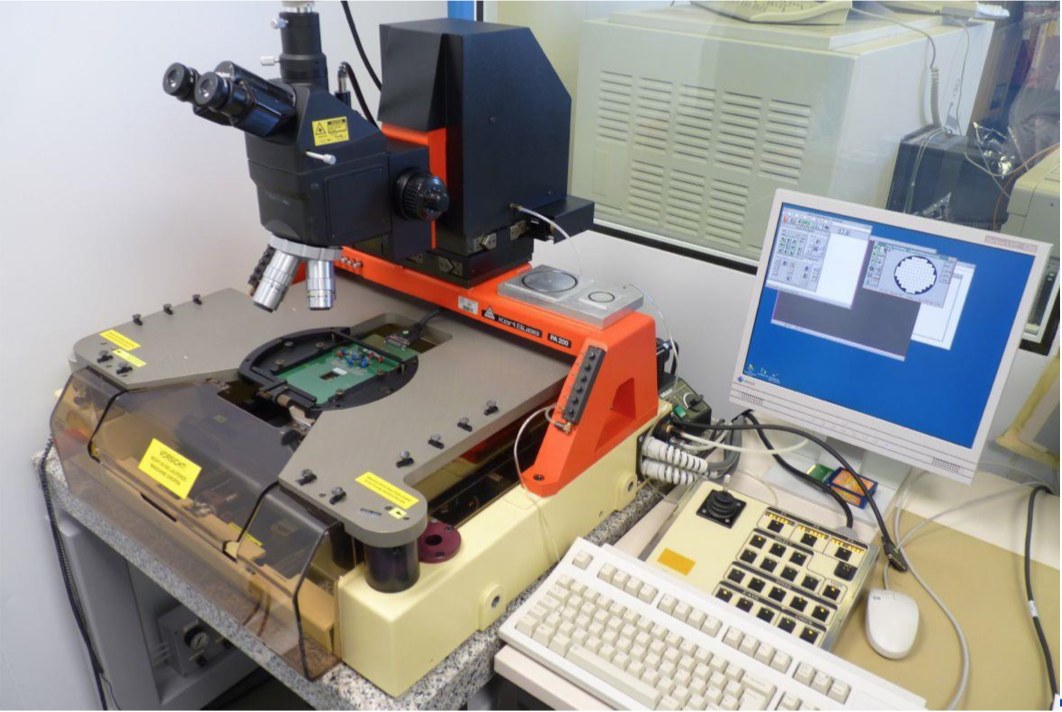
\includegraphics[width=0.49\textwidth]{figures/nsw/use_cases/verso_use_case_die_reader}}
        \caption{
            \textbf{\textit{Left}}: Silicon wafer die contianing VMM ASIC chips prior to being cut.
                Additional ASICs are shared on the same silicon wafer, as well, so as to make efficient
                use of space on the silicon and of CHFs.
            \textbf{\textit{Right}}: The silicon wafer die is inserted into the machine on the left.
                Visual inspection of the silicon can be made via the microscope.
                The machine allows for adapter boards to be used to interface to the ASICs directly,
                via the software on the PC that controls the machine.
                %Such adapter boards allowed for the VRS system to communicate with the pre-cut VMM ASICs directly
                %from the companies manufacturing the silicon dies.
        }
        \label{fig:vrs_vmm_prod}
    \end{center}
\end{figure}

\FloatBarrier


%\section{Configuration, Data-acquisition, and Calibration Software for the NSW Front-end Electronics}
%\subsection{VERSO}
%\subsection{Calibration Algorithm Development}
%\subsubsection{Gain}
%\subsubsection{ADC Calibration}
%\subsubsection{Noise Measurements}
%\subsubsection{Timing Calibration}
%\subsubsection{Per-channel Threshold Equilisation}
%\subsection{Use Cases}
%\subsubsection{Test Benches and Labs}
%\subsubsection{High Rate Tests and Test Beams}

%\section{The Upgrade of the ATLAS T/DAQ Infrastructure}
%\subsection{FELIX}
%\subsection{The Software ROD}
